\documentclass[12pt,a4paper]{report}

% ---------- Packages ----------
\usepackage[utf8]{inputenc}
\usepackage[T1]{fontenc}
\usepackage[english]{babel}
\usepackage[a4paper,margin=2.5cm]{geometry}
\usepackage{graphicx}
\usepackage{xcolor}
\usepackage{setspace}
\usepackage{titlesec}
\usepackage{hyperref}
\usepackage{float}
\usepackage{gensymb}
\usepackage{caption}
\usepackage{subcaption}
\usepackage{amsmath}
\usepackage{amssymb}
\usepackage{booktabs}
\usepackage{siunitx}
\usepackage{enumitem}
\usepackage{xcolor}
\usepackage{fancyhdr}

% ---------- Premium Academic Font Selection ----------
% Linux Libertine for text, Libertinus for Math
% This is widely considered one of the most legible and elegant academic fonts.
\usepackage{libertine}
\usepackage[libertine]{newtxmath}
\usepackage[scaled=0.95]{berasans} % Professional Sans-serif for headers
\usepackage[scaled=0.85]{beramono} % Clean monospaced for code/emails

% ---------- SIUnitx Setup ----------
\sisetup{
    detect-all,
    separate-uncertainty = true,
    exponent-product = \cdot,
    inter-unit-product = \cdot
}

% ---------- Hyperref setup ----------
\hypersetup{
    colorlinks=true,
    linkcolor=black,
    citecolor=black,
    filecolor=black,
    urlcolor=blue,
    pdftitle={Analogue Integrated Circuit Design Laboratory Report},
    pdfauthor={Amir Amaghsoud, Simone Sbrescia}
}

% ---------- Style ----------
% ---------- Clean Academic Style (IEEE-like) ----------

% Chapter style
\titleformat{\chapter}[display]
  {\normalfont\bfseries\huge}
  {\chaptername\ \thechapter}{10pt}{\Huge}

% Section style
\titleformat{\section}
  {\normalfont\bfseries\Large}
  {\thesection}{1em}{}

% Subsection style
\titleformat{\subsection}
  {\normalfont\bfseries\normalsize}
  {\thesubsection}{1em}{}

% Spacing (molto importante per look professionale)
\titlespacing*{\chapter}{0pt}{0pt}{20pt}
\titlespacing*{\section}{0pt}{15pt}{6pt}
\titlespacing*{\subsection}{0pt}{10pt}{4pt}

% Custom spacing
\setlength{\parskip}{0.8em}
\setlength{\parindent}{0pt}
\onehalfspacing

% ---------- Header / Footer ----------
\pagestyle{fancy}
\fancyhf{}
\fancyhead[L]{\small\itshape Analogue Integrated Circuit Design}
\fancyhead[R]{\small Laboratory Report}
\fancyfoot[C]{\thepage}

% ---------- Custom commands ----------

\definecolor{unipdred}{RGB}{155,0,20}
\begin{document}

% ---------- Title Page ----------
\begin{titlepage}
    \thispagestyle{empty}
    \begin{center}
    \vspace*{3cm}
    
    % Optional: Add University Logo here if you have one
    % \includegraphics[width=0.3\textwidth]{unipd_logo.png} 
    
    \vspace{1cm}

    {\huge \textbf{University of Padua}}\\[0.5cm]
    {\large Department of Information Engineering}\\[2cm]

    {\color{unipdred}\Huge \textbf{Analogue Integrated Circuit Design}}\\[0.4cm]
    {\color{unipdred}\Huge \textbf{Laboratory Sessions Report}}

    \vspace{2cm}

    {\large Academic Year 2025/2026}

    \vfill

    \begin{flushleft}
    \begin{spacing}{1.2}
    {\LARGE \textbf{Amirkhashayar Maghsoud}} \\[0.4cm]
    {\LARGE \textbf{Simone Sbrescia}}
    \end{spacing}
    \end{flushleft}
    
    \vspace{1cm}
    \end{center}
\end{titlepage}

\tableofcontents
\clearpage

% Main Content

\chapter{LAB Session 01 -- CMOS Current Mirror Design and Analysis}

\subsection*{MOSFET PARAMETERS FOR HAND CALCULATION}

\begin{center}
\resizebox{\textwidth}{!}{
\begin{tabular}{|c|c|c|c|c|c|c|}
\hline
 & $k'_{n/p}$ [$\mu$A/V$^2$] & $\eta$ [V/m] & $\chi = \frac{g_{mb}}{g_m}$ & $C_{ox}$ [fF/$\mu$m$^2$] & $C_{GS0}=C_{GD0}$ [fF/$\mu$m] & $C_{jd/s}$ [fF/$\mu$m] (*) \\
\hline
nMOSFET & 470 & $1.1 \cdot 10^7$ & 0.2 & 11.2 & 0.32 & 0.45 \\
\hline
pMOSFET & 100 & $1.5 \cdot 10^7$ & 0.2 & 11.2 & 0.32 & 0.70 \\
\hline
\end{tabular}
}
\end{center}
\vspace{0.4cm}
\subsection*{PROCESS VARIATION AND DEVICE MISMATCH PARAMETERS FOR HAND CALCULATION}

\begin{center}
\begin{tabular}{|c|c|c|c|c|}
\hline
 & $V_{TN/P}$ [V] & $k'_{n/p}$ [mA/V$^2$] & $A_{\Delta VT}$ [mV$\cdot\mu$m] & $A_{Dk/k}$ [\%\,$\cdot\mu$m] \\
\hline
nMOSFET & 
\begin{tabular}{c}
0.31 (min) \\
0.37 (typ) \\
0.44 (max)
\end{tabular}
&
\begin{tabular}{c}
376 (min) \\
470 (typ) \\
564 (max)
\end{tabular}
& 5 & 1.1 \\
\hline
pMOSFET & 
\begin{tabular}{c}
-0.26 (min) \\
-0.33 (typ) \\
-0.40 (max)
\end{tabular}
&
\begin{tabular}{c}
80 (min) \\
100 (typ) \\
120 (max)
\end{tabular}
& 3.6 & 1 \\
\hline
\end{tabular}
\end{center}

\section{Schematic and Testbench Configuration}

% Inserire schematico
\begin{figure}[H]
    \centering
    \begin{minipage}{0.48\linewidth}
        \centering
        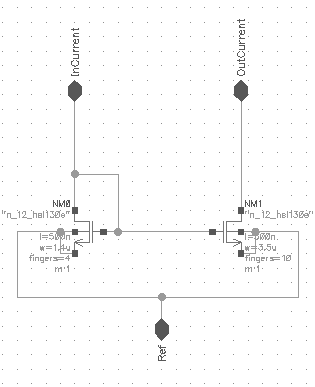
\includegraphics[width=\linewidth]{images/n_type_schematics_L500nm (1).png}
    \end{minipage}
    \hfill
    \begin{minipage}{0.48\linewidth}
        \centering
        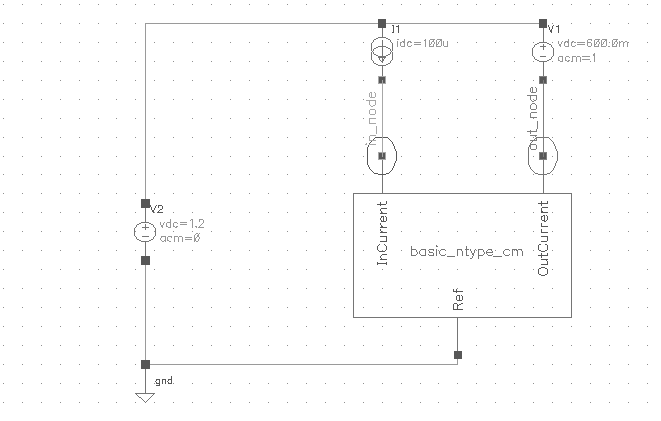
\includegraphics[width=\linewidth]{images/nmos_tb.png}
    \end{minipage}
    \caption{nMOS schematic and testbench}
\end{figure}
\section{DC and Small-Signal Characterization of the Basic Mirror}

\subsection{Output Current Behaviour Under DC Sweep}

A DC sweep of the output voltage $V1$ from 0 V to 1.2 V has been performed. The output current $I_{OUT}$ has been plotted together with the ideal mirrored current $N \cdot I_{IN}$.

\begin{figure}[H]
    \centering
    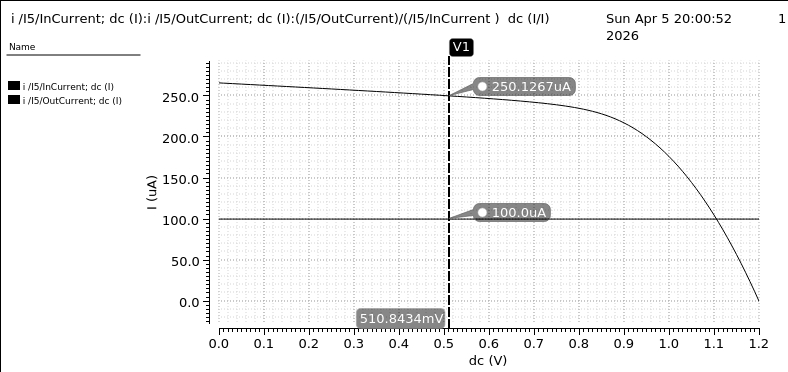
\includegraphics[width=1.0\linewidth]{images/i_o_V_i_in.jpg}
    \caption{$I_{OUT}$ vs $V_1$ with $N \cdot I_{IN}$ reference}
\end{figure}

The results show that $I_{OUT}$ initially decreases slowly and almost linearly as $V_1$ increases due to channel length modulation (CLM).
As $V_1$ increases further, the current exhibits a steeper and nonlinear decrease. In this region, the output transistor progressively leaves the saturation region and enters the triode region, leading to a more pronounced reduction of the drain current and a significant deviation from the ideal current-mirror behavior.

% Correction: Changed \begin{equation*} to \begin{equation} to match the \label and subsequent reference (\ref{eq:current_error}).
A marker has been placed at the point where $I_{OUT} = N \cdot I_{IN}$. At this point:
\begin{itemize}
    \item $V_1 = 510.84\,\text{mV}$
\end{itemize}
The equality holds only at this specific value of $V_1$ due to CLM and the originated current error can be approximated as:
\begin{equation}
\Delta I_o \approx \frac{V_{DS1} - V_{DS2}}{R_o}
\label{eq:current_error}
\end{equation}

It can be observed from (\ref{eq:current_error}) that the current error depends on the difference between $V_{DS1}$ and $V_{DS2}$. Since $V_{DS1}$ is fixed by the reference branch, while $V_{DS2}$ varies with the swept output voltage $V_1$, the condition $V_{DS1} = V_{DS2}$ is satisfied only at a single value of $V_1$. 
\subsection{Low-Frequency Output Resistance from AC Response}

An AC analysis has been carried out by applying a small-signal voltage source at the current-mirror output node, with AC magnitude equal to 1 V, around the selected DC operating point. Therefore, the magnitude and phase of the output current are respectively the magnitude and phase of the output admittance.

\begin{figure}[H]
    \centering
    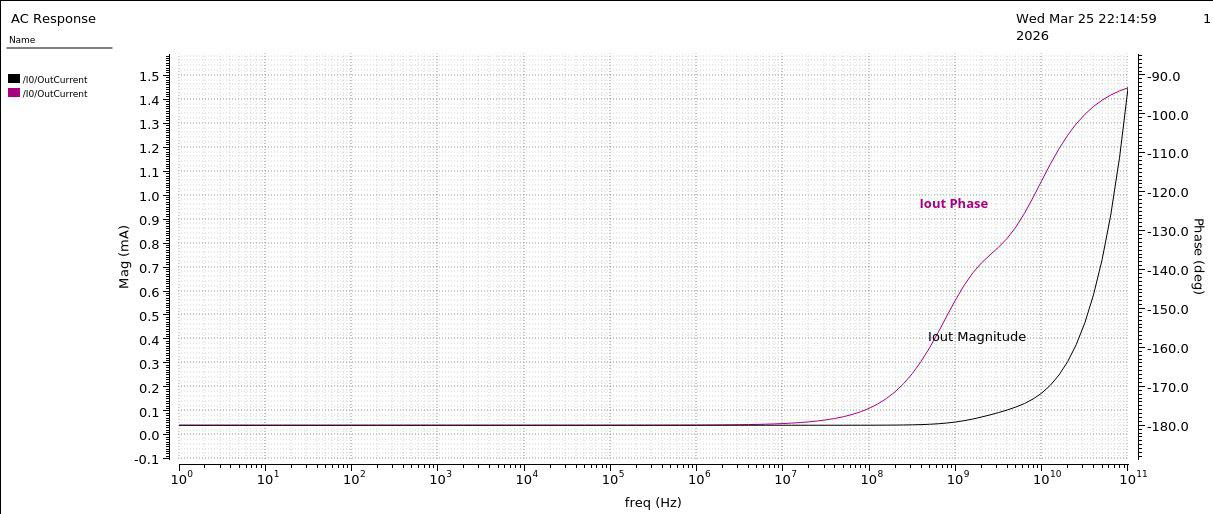
\includegraphics[width=0.8\linewidth]{images/AC phase.jpeg}
    \caption{Magnitude and phase of the output current, corresponding to the output admittance}
\end{figure}

The low-frequency value of the admittance magnitude has been extracted from the AC plot as:

\begin{equation*}
|Y_{out}(0)| \approx 39.92 \,\mu S
\end{equation*}
\begin{figure}[H]
    \centering
    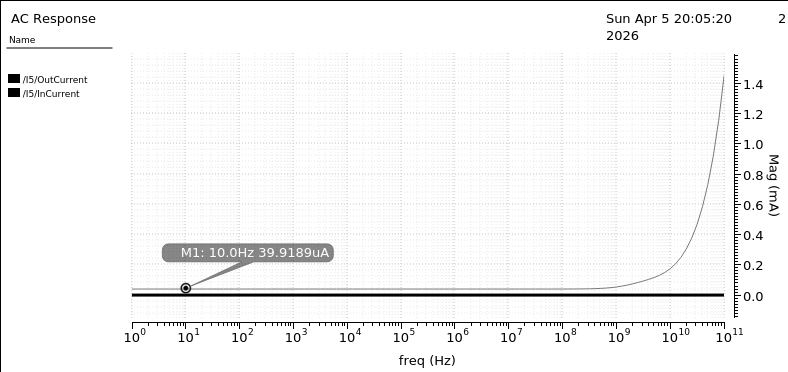
\includegraphics[width=0.8\linewidth]{imagesV2/AC_analysis_marked.jpg}
    \caption{Low-frequency value of the admittance magnitude}
\end{figure}
The corresponding output resistance is then estimated as:

\begin{equation*}
R_o = \frac{1}{|Y_{out}(0)|} \approx 25.05 \, k\Omega
\end{equation*}
This value must be compared with the output admittance obtained from the DC sweep. In particular, the small-signal admittance at DC is given by the local slope of the $I_{OUT}$--$V_1$ characteristic, evaluated at the same operating point used for the AC simulation:
\begin{equation*}
Y_{out}(0)=\left.\frac{dI_{OUT}}{dV_1}\right|_{Q=510.84mV}=34.82\mu S
\end{equation*}
The relative error between the two estimations is:

\begin{equation*}
\text{Error} = \frac{|Y_{out}^{AC} - Y_{out}^{DC}|}{Y_{out}^{AC}} \approx 12.8\%
\end{equation*}
The discrepancy between the AC and DC result is primarily 
attributed to the mismatch in the operating point ($Q$-point). In the AC 
calculations, the operating point was constrained by the fixed DC voltage 
connected to the output node, where $V_{DC} = 600 \, \text{mV}$. 

Conversely, the precise operating point of the MOSFET was determined to be 
$510.84 \, \text{mV}$, corresponding to the condition $I_o = 2.5 I_{in}$. 
Although quantization steps in the simulation prevented the evaluation of the 
exact point where the current ratio perfectly matches the ideal value, this 
quantization error is negligible. The primary source of divergence is the 
offset between the software's operating point and the analytical operating 
point used in the admittance derivation.
\subsection{Output impedance frequency behaviour}
According to the small-signal equivalent circuit, the output impedance can be modeled as:

\begin{equation*}
Z_{out}(s)=\frac{r_{o2}}{1+s r_{o2}[C_{db2}+(N+1)C_{gd2}]}
\end{equation*}
Where the intersted parasitic capacitances are evaluated from process parameters as:

\begin{equation*}
C_{gd2} = C_{gd0}\cdot W = 0.32\,\frac{\text{fF}}{\mu m} \cdot 3.5\,\mu m = 1.12\,\text{fF}
\end{equation*}

\begin{equation*}
C_{db2} = C_{jn}\cdot W = 0.45\,\frac{\text{fF}}{\mu m} \cdot 3.5\,\mu m =1.58\,\text{fF}
\end{equation*}

The dominant pole of the output impedance is therefore:
\begin{equation*}
f_p = \frac{1}{2\pi r_{o2}\left[C_{db2}+(N+1)C_{gd2}\right]} \approx 1.318\,\text{GHz}
\end{equation*}
\begin{figure}[H]
    \centering
    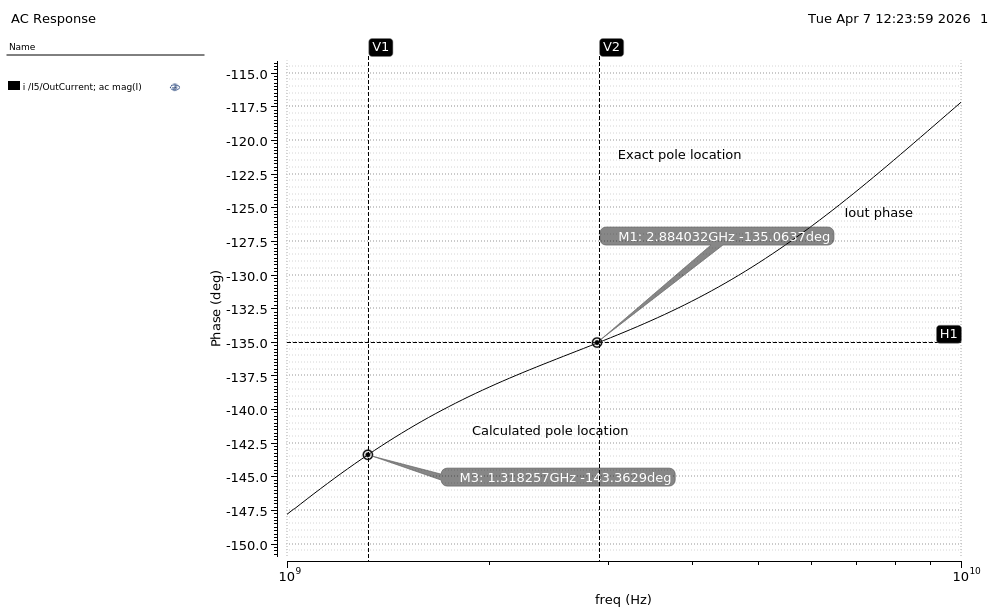
\includegraphics[width=1.0\linewidth]{imagesV2/phase_mag_annot_exact.png}
    \caption{Phase response of the output admittance. Markers highlight the theoretical pole}
\end{figure}
The theoretical behavior of the output impedance is confirmed by the simulation results. At low frequency, the output impedance is purely resistive and approximately equal to $r_{o2}$, corresponding to the flat region observed in the AC response.
The phase response is also consistent with the theoretical model. In particular, a phase shift is observed around the pole frequency, marking the transition from resistive to capacitive behavior.
From the phase plot, the actual pole frequency can be identified as the point where the phase reaches approximately $-135^\circ$. From the simulation results, this occurs at:
\begin{equation*}
f_{p,real} = 2.88\,\text{GHz}
\end{equation*}
The discrepancy between the theoretical and simulated pole frequencies is mainly due to parasitic capacitances and higher-order effects, which are not fully captured by the simplified analytical model.
\subsection{DC Analysis with Gate Length and Finger Width Variations}
First, the effect of the gate length has been investigated. The minimum and maximum values have been set to $L_{min} = 100\,\text{nm}$ and $L_{max} = 500\,\text{nm}$, respectively. The simulator automatically selected 10 intermediate points within this range, allowing to highlight the dependence of the output current on the transistor channel length.

\begin{figure}[H]
    \centering
    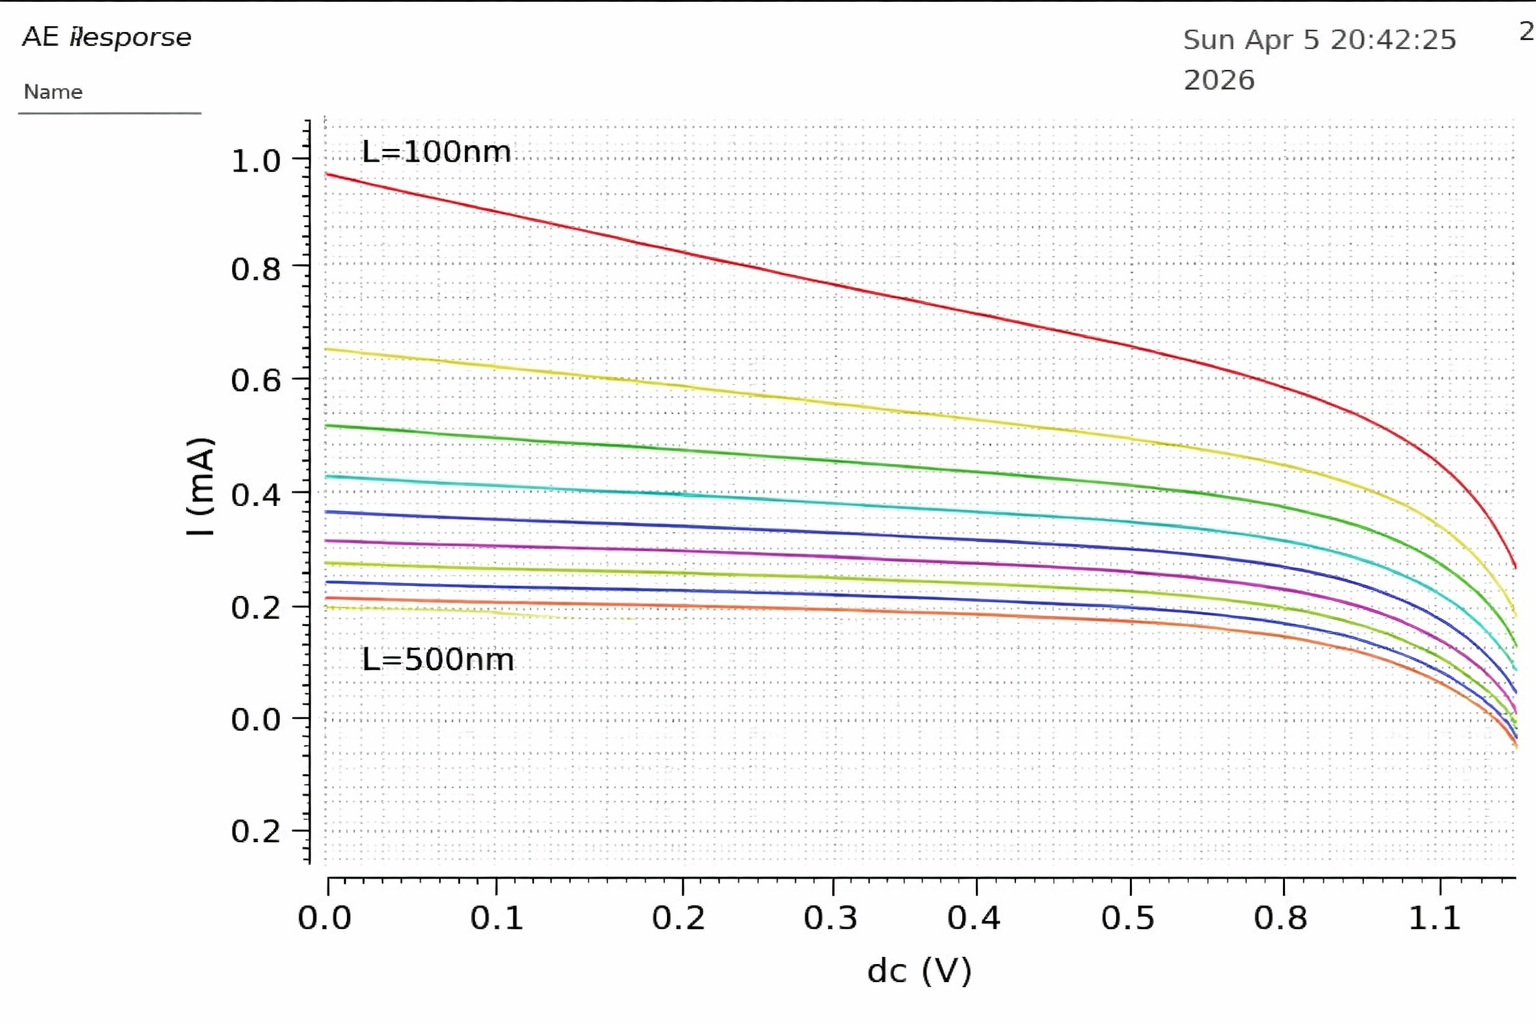
\includegraphics[width=0.82\linewidth]{images/Curva di corrente per lunghezze canale.png}
    \caption{DC output current $I_{OUT}$ as a function of the output voltage for different values of the gate length $L$, ranging from $100\,\text{nm}$ to $500\,\text{nm}$. The curves show how the transistor length affects the output current.}
    \label{fig:cm_dc_variants}
\end{figure}

\begin{figure}[H]
    \centering
    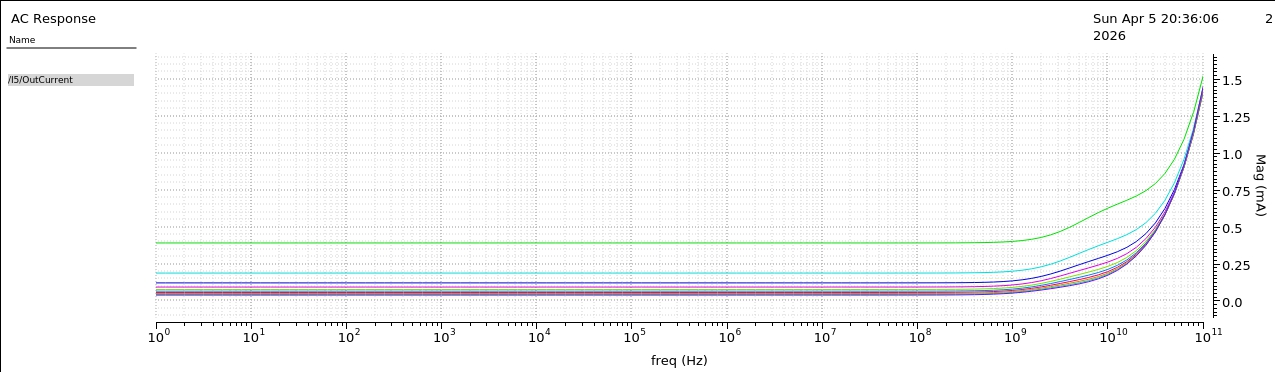
\includegraphics[width=1.00\linewidth]{imagesV2/I_o_ac_DiffrentL.jpg}
    \caption{AC response of the current mirror for different gate lengths $L$.}
    \label{fig:cm_ac_variants}
\end{figure}

In a second step, the effect of transistor layout has been analyzed by varying the number of fingers of transistor $M_2$. In particular, two configurations have been considered: 4 fingers and 10 fingers, keeping the total width and length consistent with the original design.

\begin{figure}[H]
    \centering
    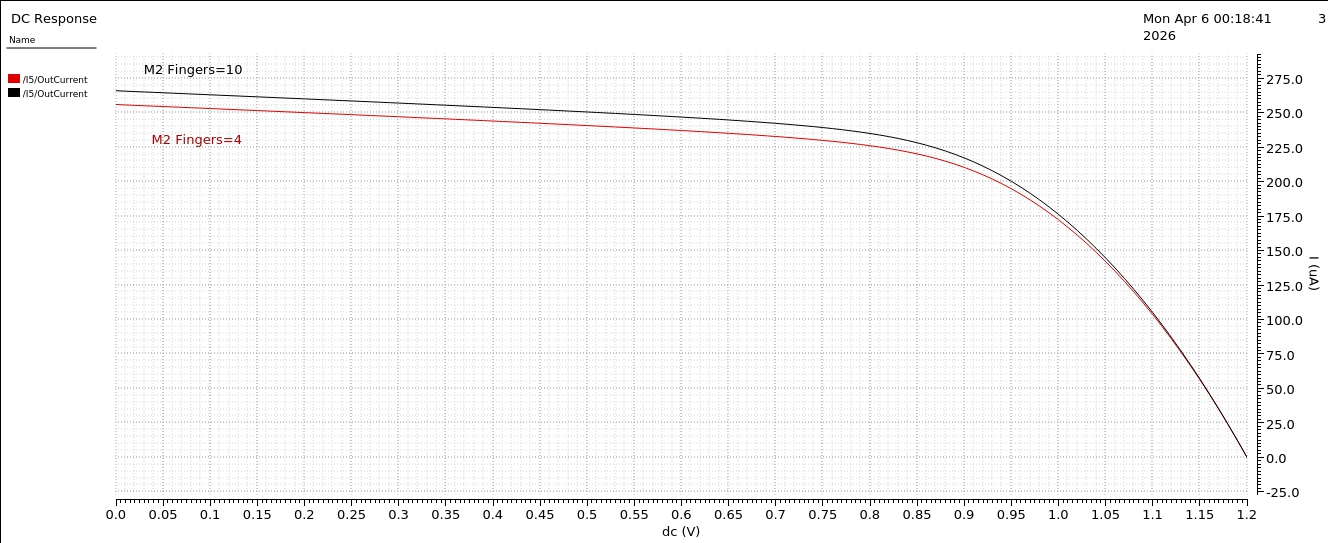
\includegraphics[width=0.82\linewidth]{imagesV2/DC4-10.jpg}
    \caption{DC output characteristics of the current mirror for two different finger configurations of $M_2$ (4 and 10 fingers).}
    \label{fig:4_10dc_variants}
\end{figure}

\begin{figure}[H]
    \centering
    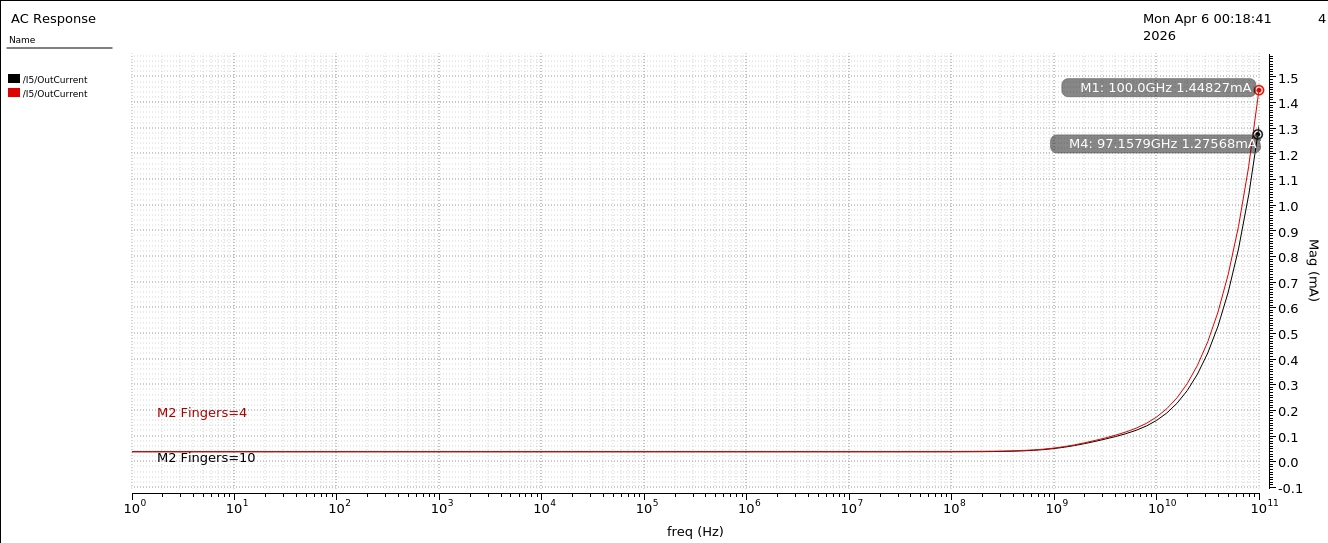
\includegraphics[width=0.82\linewidth]{imagesV2/AC4-10.jpg}
    \caption{AC response of the current mirror for different finger configurations of $M_2$ (4 and 10 fingers).}
    \label{fig:4_10ac_variants}
\end{figure}
\subsubsection{Discussion of Results}
\paragraph{Effect of $L_1\neq L_2$:}
It is important to distinguish the role of the two transistors in this analysis. For $M_1$, the reference current $I_{REF}$ is externally imposed and fixed to $100\,\mu\text{A}$. In contrast, for $M_2$ the drain current is not imposed, but results from the mirror action and from the actual device geometry. Therefore, when the channel length of $M_2$ is reduced, the output current $I_O$ increases, and this is consistent with the MOS saturation-current expression:
\begin{equation*}
I_D \approx \frac{1}{2}\mu C_{ox}\frac{W}{L}(V_{GS}-V_{th})^2(1+\lambda V_{DS}),
\end{equation*}
because a shorter channel directly increases the factor $W/L$. In addition, in the considered range the threshold voltage of $M_2$ also changes with $L$, but the sweep shows that the dominant effect on the current is the explicit dependence on $1/L$ in the previous equation. As a result, shorter values of $L_2$ produce larger values of $I_O$.

%\begin{figure}[H]
 %   \centering
  %  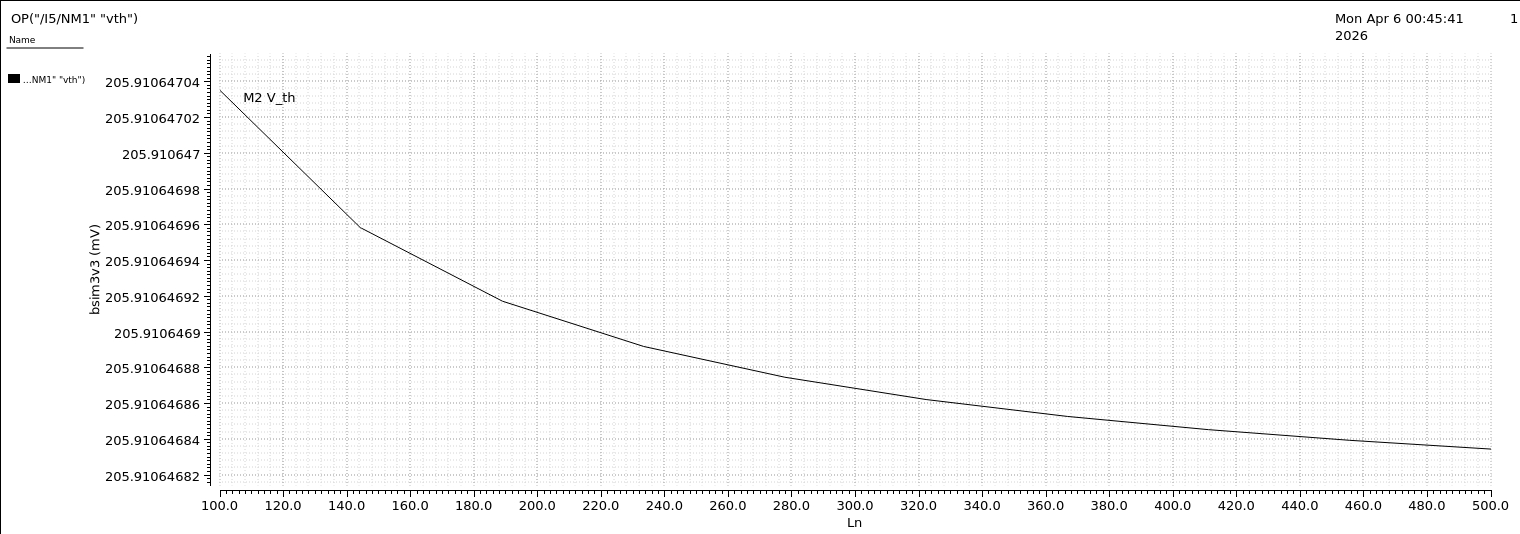
\includegraphics[width=0.8\linewidth]{images/Vth_L.jpg}
   % \caption{Sweep of the channel length of $M_2$ and corresponding variation of its threshold voltage $V_{th,2}$.}
    %\label{fig:M2_L_Vth_sweep}
%\end{figure}
\paragraph{Effect of different number of fingers for M2:}
A similar interpretation applies to the case with a different number of fingers. According to the qualitative plot of $V_T$ versus $W$ at fixed $L$, the threshold voltage also depends (although more weakly) on the effective device width. Changing the number of fingers modifies how the total width is physically distributed, thus altering the effective geometry of the transistor and introducing layout-dependent effects. In the considered case (Number of Fingers = 4 for $M_2$), the output current curve deviates from the nominal one even though the overall $W$ and $L$ are kept consistent with the original design. This is because the different finger configuration changes the effective threshold voltage and the parasitic elements of the device. As a result, the current mirror no longer perfectly replicates the reference current, and a visible deviation appears along the entire sweep. Compared to the channel length variation, this effect is generally smaller, but still significant, confirming that both device geometry and layout implementation impact the accuracy of the current mirror.



\section{Assessment of process spread and device mismatch }
Process corner simulations have been performed for the following conditions: Typical (TYP, 27°C), Slow-Slow (SS, -20°C), and Fast-Fast (FF, 85°C).

\subsection{Process Corner Evaluation}

\begin{table}[h!]
\centering
\caption{Current Mirror Performance Across Process Corners}
\label{table:corners_corrected}
\begin{tabular}{|l|c|c|}
\hline
\textbf{Corner} & \textbf{$V_{IN}$ [mV]} & \textbf{$\Delta I_{OUT}$ [$\mu$A]} \\ \hline
TYP (27 °C)     & 686.0                  & -3.096                             \\ \hline
SS (-20 °C)     & 751.4                  & -5.516                             \\ \hline
FF (85 °C)      & 630.8                  & -1.155                             \\ \hline
\end{tabular}
\end{table}




The variations observed in $V_{IN}$ and $\Delta I_{OUT}$ across the simulated process corners (\textbf{TYP}, \textbf{SS}, and \textbf{FF}) are primarily driven by the global fluctuations in the threshold voltage ($V_{th}$) and carrier mobility ($\mu$). These dependencies are governed by the MOSFET saturation current equation:

\begin{equation*}
I_D \approx \frac{1}{2} \mu C_{ox} \frac{W}{L} (V_{GS} - V_{th})^2 (1 + \lambda V_{DS})
\end{equation*}
\subsubsection{Discussion of Results}
\paragraph{Input Voltage ($V_{IN}$) Sensitivity}:
In the \textbf{SS (Slow-Slow)} corner at \textbf{$-20$°C}, the devices show the highest threshold voltage and degraded mobility. To hold the fixed reference current of $100\,\mu$A, the gate-source voltage ($V_{GS} = V_{IN}$) must increase to compensate for the "weak" drive capability. This resulted in the observed maximum $V_{IN}$ of \textbf{751.4\,mV}. 

Conversely, in the \textbf{FF (Fast-Fast)} corner at \textbf{85°C}, the significant reduction in $V_{th}$ dominates the temperature-induced mobility decrease. Consequently, the transistors reach the target current with a lower overdrive voltage, leading to a minimum $V_{IN}$ of \textbf{630.8\,mV}. The total spread of \textbf{120.6\,mV} represents the impact of global process and temperature variation on the biasing point.



\paragraph{Output Current Error ($\Delta I_{OUT}$)}:

For an n-type current mirror, the relationship between the reference current ($I_{REF}$) and the output current ($I_{OUT}$) is defined by the aspect ratios and the channel length modulation effect:

\begin{equation*}
I_{OUT} = N \cdot I_{REF} \cdot \frac{1 + \lambda V_{DS2}}{1 + \lambda V_{DS1}}
\end{equation*}

where $N = 2.5$ and $I_{REF} = 100\,\mu$A, yielding an ideal $I_{OUT}$ of $250\,\mu$A. The current error is defined as $\Delta I_{OUT} = I_{OUT} - 250\,\mu$A. The simulation results show:

\begin{itemize}
    \item \textbf{Negative Error Trend:} The error remains negative across all corners, indicating $I_{OUT} < 250\,\mu$A. This suggests that $V_{DS1} > V_{DS2}$ in the DC operating point, or that the effective $\lambda$ at these lengths reduces the output current more than predicted.
    
    \item \textbf{SS Corner ($-5.516\,\mu$A):} At $-20$°C, the transistors exhibit lower channel length modulation ($\lambda$) but higher $V_{th}$ mismatch sensitivity. The larger error magnitude suggests a significant discrepancy between the drain-source voltages of the mirror pair at this cold temperature.
    
    \item \textbf{FF Corner ($-1.155\,\mu$A):} The error is minimized under "fast" conditions at $85$°C. This is due to the higher transconductance ($g_m = \mu C_{ox} \frac{W}{L}(V_{GS}-V_{th})$) of the devices, which makes the output current more robust against small voltage offsets between the input and output nodes.
\end{itemize}
\subsection{Monte Carlo Analysis of Current and Input-Voltage Spread}

A Monte Carlo simulation ($N=100$) was performed to evaluate the impact of local device mismatch and global process variations on the current mirror's performance. The extracted mean values ($\mu$) and standard deviations ($\sigma$) from these distributions are summarized in Table \ref{table:monte_carlo}.

\begin{figure}[H]
    \centering
    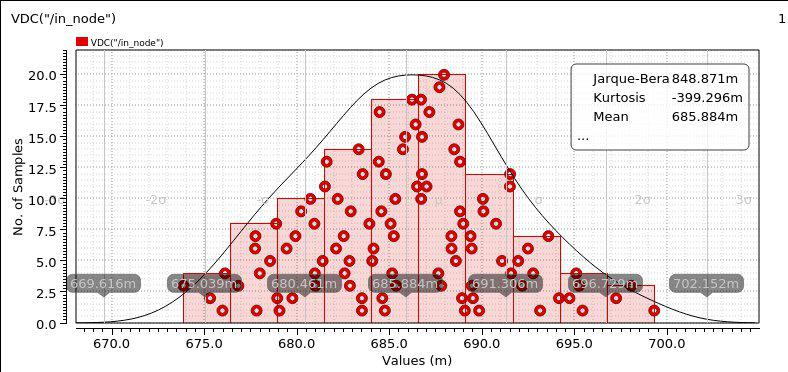
\includegraphics[width=0.8\linewidth]{images/vcd_montecarlo.JPG}
    \caption{Monte Carlo distribution of $V_{IN}$.}
    \label{fig:vcd_montecarlo}
\end{figure}

\begin{figure}[H]
    \centering
    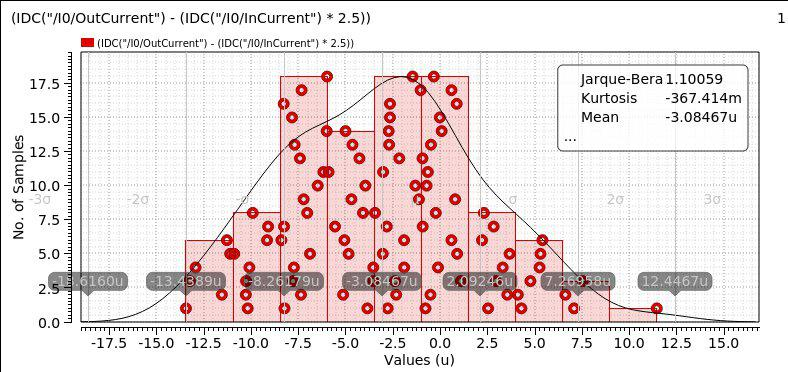
\includegraphics[width=0.8\linewidth]{images/currents_montecarlo.JPG}
    \caption{Monte Carlo distribution of $\Delta I_{OUT}$.}
    \label{fig:currents_montecarlo}
\end{figure}

\begin{table}[h!]
\centering
\caption{Monte Carlo Statistical Results ($N=100$)}
\label{table:monte_carlo}
\begin{tabular}{|l|c|c|}
\hline
\textbf{Variable} & \textbf{Mean} & \textbf{Std. Deviation ($\sigma$)} \\ \hline
Input Voltage $V_{IN}$ [mV]     & 685.88                & 5.42                               \\ \hline
Current Error $\Delta I_{OUT}$ [$\mu$A] & -3.085                   & 5.18                               \\ \hline
\end{tabular}
\label{Fig:table_montecarlo}
\end{table}
\paragraph{Systematic vs. Random Error}
As observed in the histograms, the mean value of the current error $\Delta I_{OUT}$ is $-3.085\,\mu$A rather than zero. This represents the \textbf{systematic error} of the design, primarily caused by the $V_{DS}$ mismatch between the input and output branches of the simple current mirror. The standard deviation $\sigma = 5.18\,\mu$A represents the random mismatch inherent in the manufacturing process.

\paragraph{Mismatch Verification}
To verify the consistency of the simulation, the Pelgrom mismatch model is applied using the parameters $A_{\Delta VT} = 5\,\text{mV}\cdot\mu\text{m}$ and $A_{Dk/k} = 1.1\,\%\cdot\mu\text{m}$. For a device area $W \cdot L = 1.75\,\mu\text{m}^2$:

\begin{equation*}
\sigma_{\Delta VT} = \frac{A_{\Delta VT}}{\sqrt{W \cdot L}} = 3.78\,\text{mV}, \quad \sigma_{\Delta k/k} = \frac{A_{Dk/k}}{\sqrt{W \cdot L}} = 0.0083
\end{equation*}

The total relative current mismatch is estimated as:
\begin{equation*}
\sigma_{\Delta I/I} = \sqrt{\sigma_{\Delta k/k}^2 + \left( \frac{2}{V_{GS} - V_{th}} \sigma_{\Delta VT} \right)^2} \approx 2.53\%
\end{equation*}

For an ideal $I_{OUT} = 250\,\mu$A, the calculated standard deviation is:
\begin{equation*}
\sigma_{calc} = 250\,\mu\text{A} \cdot 0.0253 = 6.32\,\mu\text{A}
\end{equation*}

\paragraph{Comparison of Statistical and Deterministic Distributions}

A critical comparison is made between the global process corners and the local statistical variations. For the input bias voltage $V_{IN}$, the Monte Carlo simulation yielded a standard deviation $\sigma_{V_{IN}} = 5.42\,\text{mV}$. The $3\sigma$ confidence interval, which covers $99.7\%$ of the statistical samples, is calculated as:
\begin{equation*}
\Delta V_{IN, 3\sigma} = 6 \cdot \sigma_{V_{IN}} = 6 \cdot 5.42\,\text{mV} \approx 32.52\,\text{mV}
\end{equation*}

In contrast, the deterministic corner analysis (from SS at $-20^\circ$C to FF at $85^\circ$C) showed a spread of:
\begin{equation*}
\Delta V_{IN, corners} = V_{IN,SS} - V_{IN,FF} = 751.4\,\text{mV} - 630.8\,\text{mV} = 120.6\,\text{mV}
\end{equation*}
Regarding the output current accuracy, the simulated standard deviation of the error $\sigma_{\Delta I, sim} = 5.18\,\mu$A was compared to the Pelgrom calculation derived earlier:
\begin{equation*}
\sigma_{\Delta I, calc} = I_{OUT, ideal} \cdot \sqrt{\frac{A_{Dk/k}^2}{WL} + \left( \frac{2}{V_{OV}} \frac{A_{\Delta VT}}{\sqrt{WL}} \right)^2} \approx 6.32\,\mu\text{A}
\end{equation*}

\section{Wide-Swing Cascode Current Mirror (WS-CCM)}

\subsection{Schematic and Testbench Configuration}

The wide-swing cascode current mirror (WS-CCM) has been implemented according to the design specifications. The circuit schematic and the corresponding testbench are shown in Fig.~\ref{fig:cascode_schematic_tb}.

\begin{figure}[H]
    \centering
    \begin{minipage}{0.46\linewidth}
        \centering
        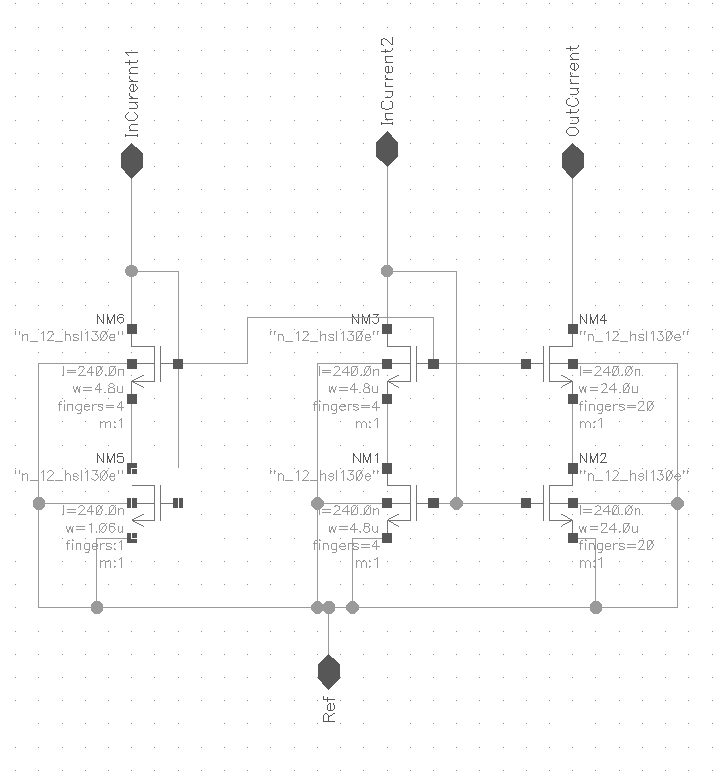
\includegraphics[width=\linewidth]{imagesV2/schematics_w_1.06.png}
    \end{minipage}
    \hfill
    \begin{minipage}{0.46\linewidth}
        \centering
        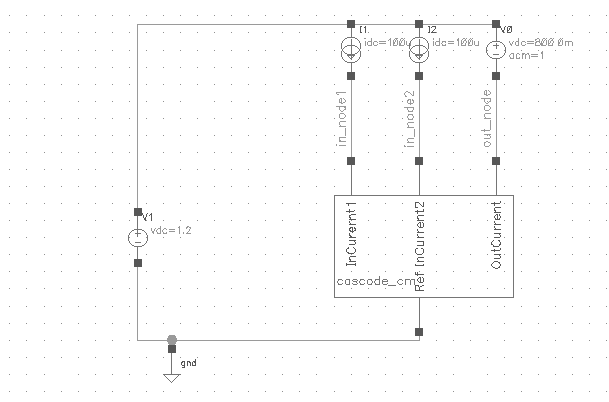
\includegraphics[width=\linewidth]{imagesV2/tb_cascode_schematics (1).png}
    \end{minipage}
    \caption{WS-CCM schematic (left) and testbench (right)}
    \label{fig:cascode_schematic_tb}
\end{figure}

\subsection{Operating Point Adjustment}

A parametric sweep of the transistor $M_5$ width has been performed in order to properly bias the circuit. The final value has been selected as the point at which the family of curves corresponding to $V_{DS1}$, $V_{DS2}$, $V_{DS3}$ and $V_{DS4}$ is overall closest to the target value of $0.25\,\text{V}$.

The final selected value is:

\begin{equation*}
W_{M5} = 1.06\,\mu\text{m}, \quad L_{M5} = 240\,n\text{m}
\end{equation*}
\begin{figure}[H]
    \centering
    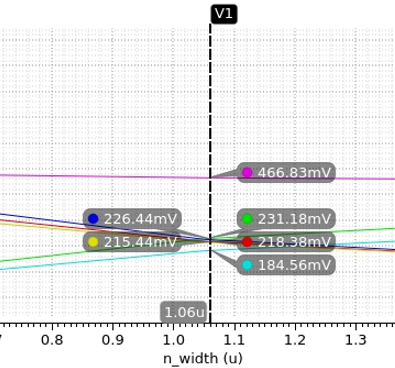
\includegraphics[width=0.5\linewidth]{imagesV2/Screenshot 2026-04-04 100809.png}
    \caption{Family of curves of $V_{DS1}$, $V_{DS2}$, $V_{DS3}$ and $V_{DS4}$ as a function of $W_5$.}
    \label{fig:vds_sweep}
\end{figure}

\begin{figure}[H]
    \centering
    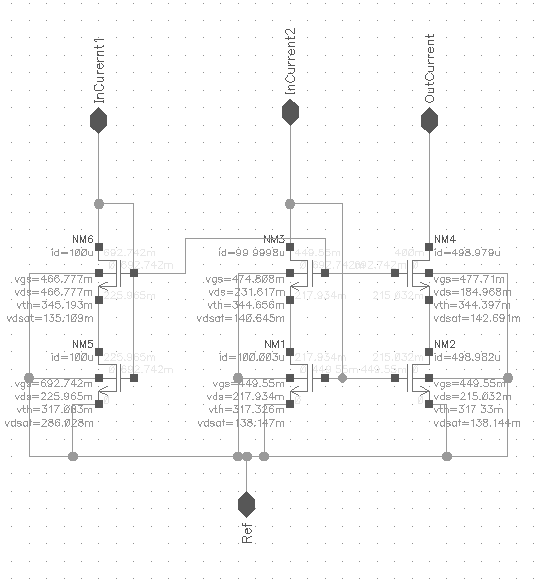
\includegraphics[width=0.65\textwidth]{chapters/M5_op.png} 
    \caption{Cascode schematics with operating points and node voltages.}
    \label{fig:cascode_op}
\end{figure}

The resulting operating point values for the cascode current mirror are summarized in Table 1.3:

\begin{table}[H]
    \centering
    \caption{Measured DC Operating Point Parameters}
    \label{table:operating_points}
    \begin{tabular}{lc}
        \toprule
        \textbf{Parameter} & \textbf{Value [mV]} \\
        \midrule
        $V_{DS1}$          & 226.44              \\
        $V_{DS2}$          & 215.40              \\
        $V_{DS3}$          & 231.20              \\
        $V_{DS4}$          & 184.60              \\
        $V_{G6}$           & 692.74              \\
        \bottomrule
    \end{tabular}
\end{table}
The selection of the optimal value of $W_5$ is driven by a design trade-off. In principle, it would have been possible to choose a point where $V_{DS1}$ and $V_{DS2}$ are exactly equal to $250\,\text{mV}$. However, in that case, $V_{DS3}$ and $V_{DS4}$ would have deviated significantly from the target value of $250\,\text{mV}$. Therefore, a compromise solution has been adopted, selecting the value of $W_5$ for which all four drain-source voltages are as close as possible to the desired target simultaneously.

\subsection{DC Sweep Analysis}

A DC sweep of the output voltage $V_{OUT}$ has been performed. The resulting output current $I_{OUT}$ has been compared with the ideal mirrored current:

\begin{figure}[H]
    \centering
    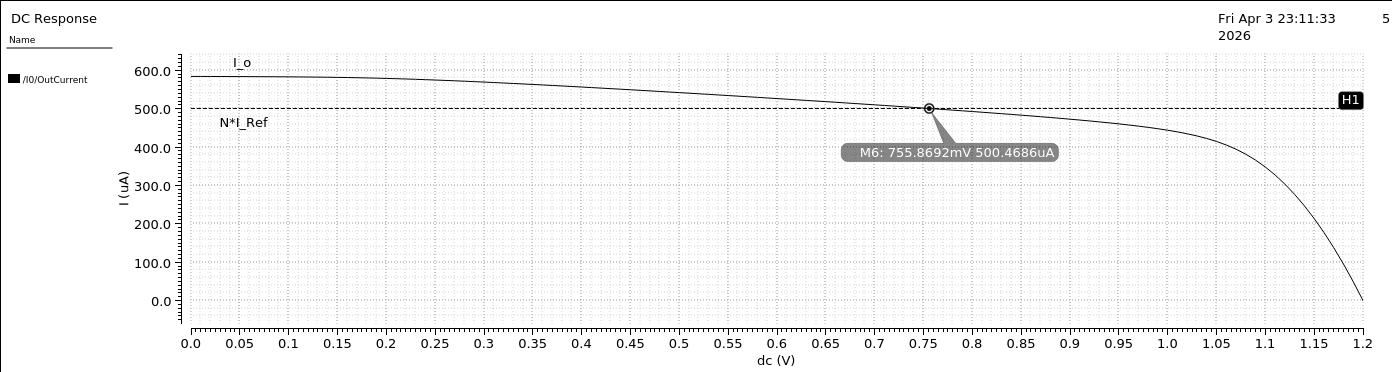
\includegraphics[width=1.00\linewidth]{imagesV2/I_o_vs_I_ref.jpg}
    \caption{DC sweep: $I_{OUT}$ and ideal current comparison with marker}
\end{figure}

\subsection{AC Analysis and Output Resistance}

An AC analysis has been carried out by applying a small-signal excitation of 1 V at the output node. Under this condition, the output current corresponds to the output admittance as it happened for the CM:

\begin{figure}[H]
    \centering
    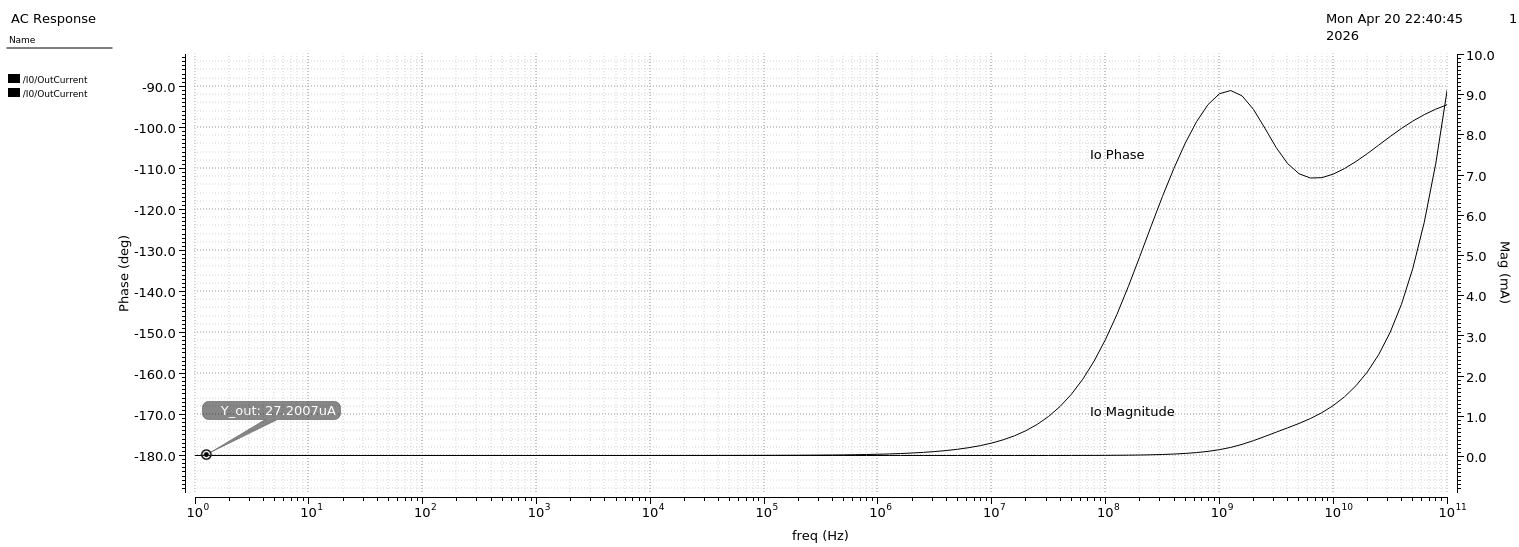
\includegraphics[width=0.8\linewidth]{chapters/miagesredone/Io_phase_mag.png}
    \caption{Magnitude and phase of the small signal output current}
\end{figure}

From the low-frequency value of the admittance magnitude:

\begin{equation*}
|Y_{out}(0)| = 27.2\,\mu\text{S}
\end{equation*}
the output resistance is then estimated as:

\begin{equation*}
R_o = \frac{1}{|Y_{out}(0)|} = 36.76\,\text{k}\Omega
\end{equation*}

\subsection{Output current error}
A DC sweep of the output voltage $V_{OUT}$ has been performed. First, the quantity $|V_{OUT} - V_{IN}|$ has been plotted as a function of $V_{OUT}$. Then, the output current error $|I_{OUT} - 5I_{REF}|$ has been plotted over the same sweep.

The operating point is identified as the value of $V_{OUT}$ for which the condition $|V_{OUT} - V_{IN}| = 0.4\,\text{V}$ is satisfied. By placing markers on the corresponding points of the two plots, the output current error is graphically extracted at the required condition.
% Missing \caption element inside
\begin{figure}[H]
    \centering
    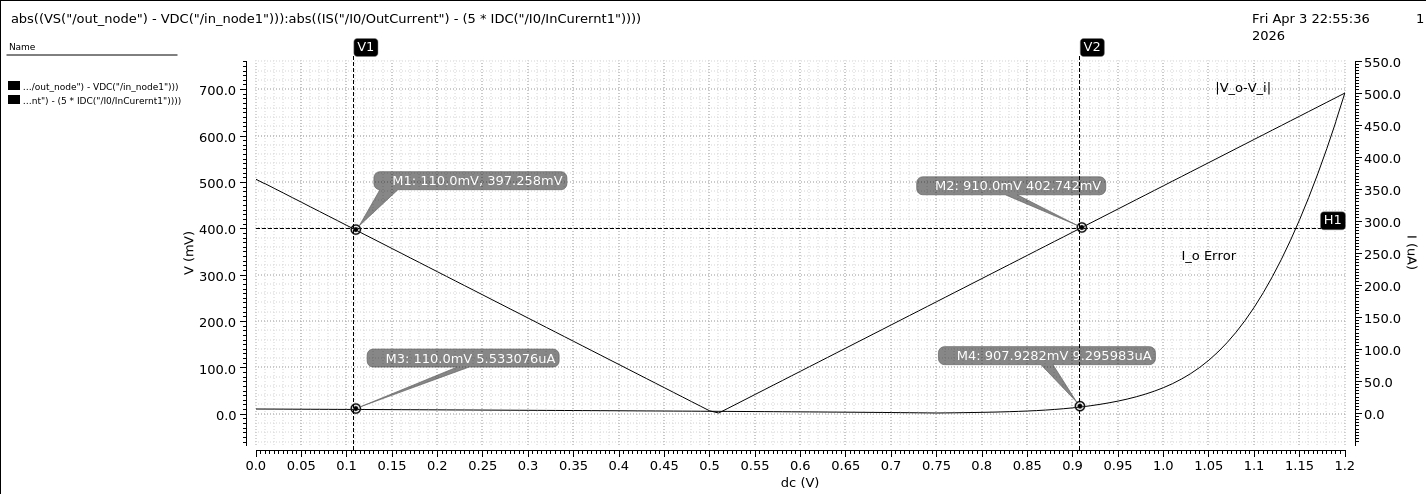
\includegraphics[width=1.00\linewidth]{imagesV2/part3_final.jpg}
    \caption{Output current error $|I_{OUT} - 5I_{REF}|$ and voltage deviation $|V_{OUT} - V_{IN}|$ vs $V_{OUT}$.}
    \label{fig:current_error}
\end{figure}
\subsubsection{Interpretation of the Current Error}
Although two operating points satisfy the required condition, only the right one on the graph(corresponding to the higher value of $V_{OUT}$) is physically meaningful. The first point occurs at low $V_{OUT}$, where the transistors are close to leaving the saturation region, thus violating the proper operating conditions of the current mirror.

Therefore, the current error is evaluated at the second intersection point, where the circuit operates correctly in saturation. The extracted value is:

\begin{equation*}
\Delta I_{OUT} \approx 9.3\,\mu\text{A}
\end{equation*}
In order to increase the output resistance of the cascode current mirror, the transistor dimensions have been scaled.
\subsection{Sizing approach for output resistance optimization}
Since the output resistance can be approximated as:
\begin{equation*}
R_o \approx g'_{m4} \cdot r_{o4} \cdot r_{o2}
\end{equation*}
it follows that, for constant current, the output resistance scales approximately as:
\begin{equation*}
R_o \propto L^2
\end{equation*}

For this reason, a first scaling factor $k = \sqrt{3}$ has been considered. This value is derived from the theoretical quadratic dependence of $R_o$ on the channel length and therefore represents only an ideal estimation.

The channel lengths of all transistors ($M_1$--$M_6$) have been increased by this factor. In order to preserve the aspect ratios and avoid modifying the bias currents, the widths have also been scaled accordingly for all transistors except $M_5$.

For transistor $M_5$, which acts as a biasing device, a rule-of-thumb has been adopted:
\begin{equation*}
W_5 = \frac{W_6}{3}
\end{equation*}

This choice allows proper biasing of the cascode branch. The operating point confirms that all transistors remain in saturation, including $M_5$.

\vspace{0.3cm}

From a theoretical point of view:
\begin{equation*}
R_o^{(th)} = 3 \cdot R_o = 3 \cdot 36.76\,\text{k}\Omega \approx 110\,\text{k}\Omega
\end{equation*}

However, simulation results show a different behaviour. From the AC analysis, the low-frequency output admittance is:
% Measunmet unit was A
\begin{equation*}
Y_{out}^{(sim)}(0) = 6.81\,\mu\text{S}
\end{equation*}
from which the output resistance is extracted as:
\begin{equation*}
R_o^{(sim)} = \frac{1}{Y_{out}^{(sim)}(0)} \approx 146.8\,\text{k}\Omega
\end{equation*}

This result highlights a deviation from the simplified model. However, the achieved design shows that both the systematic error and the mismatch of the output current are significantly reduced. This improvement comes at the cost of an increased occupied area (factor of $2.25$) coming with parasitic capacitances.

\begin{figure}[H]
    \centering
    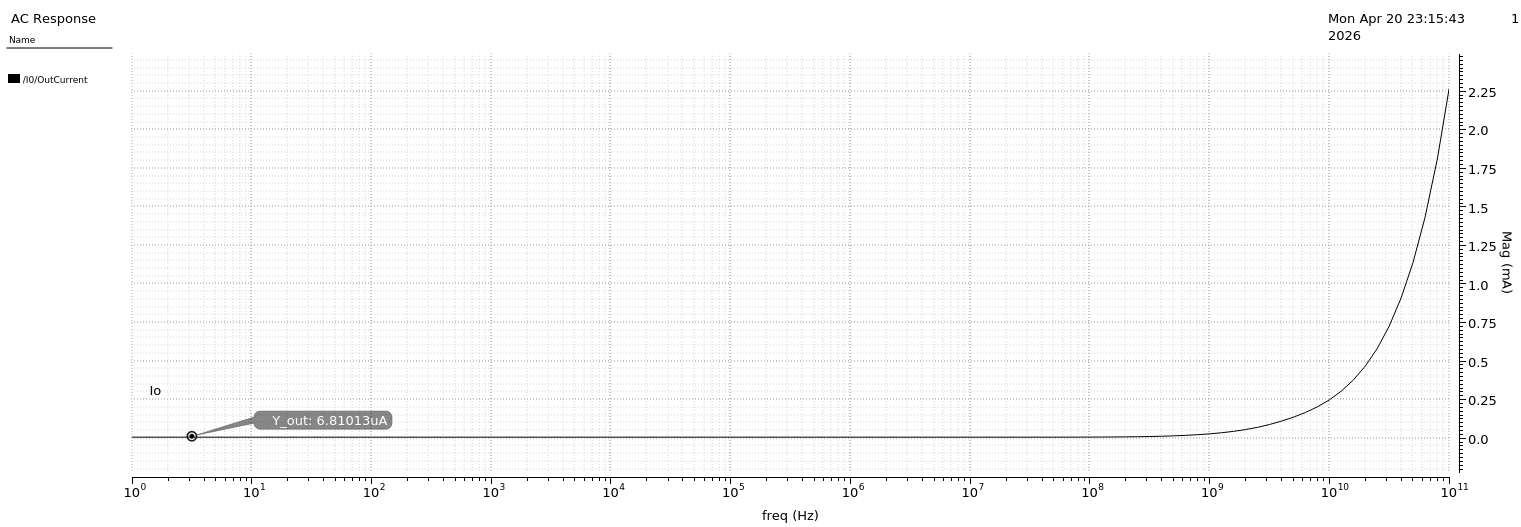
\includegraphics[width=1.0\linewidth]{chapters/miagesredone/Io_mag_cascode.png}
    \vspace{0.4cm}
    
    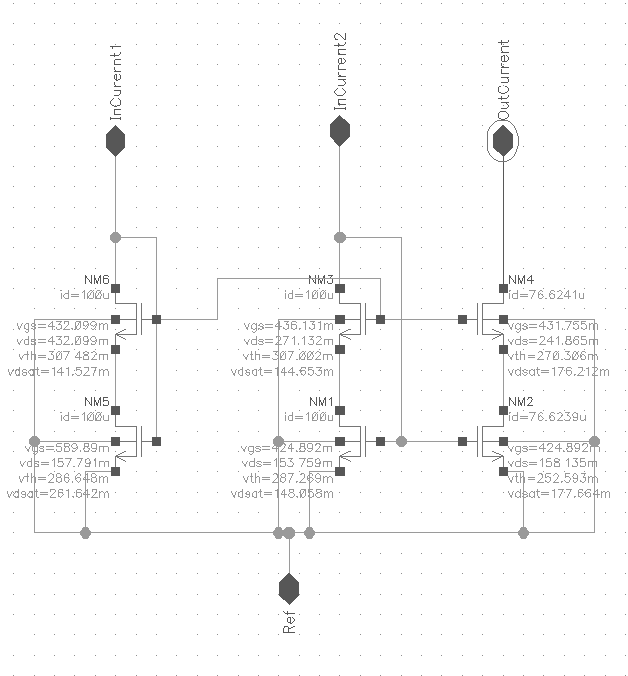
\includegraphics[width=0.6\linewidth]{chapters/miagesredone/schematics_cascode_op.png}
    
    \caption{Top: AC response used to extract the output admittance and compute $R_o^{(sim)}$. Bottom: operating point of the cascode mirror, showing that transistor $M_5$ is correctly biased in saturation.}
    \label{fig:cascode_rematch}
\end{figure}
\chapter{LAB Session 02 -- Fully Differential Current-Mirror OTA}
\section{Schematic and Testbench Configuration}
\begin{figure}[H]
    \centering
    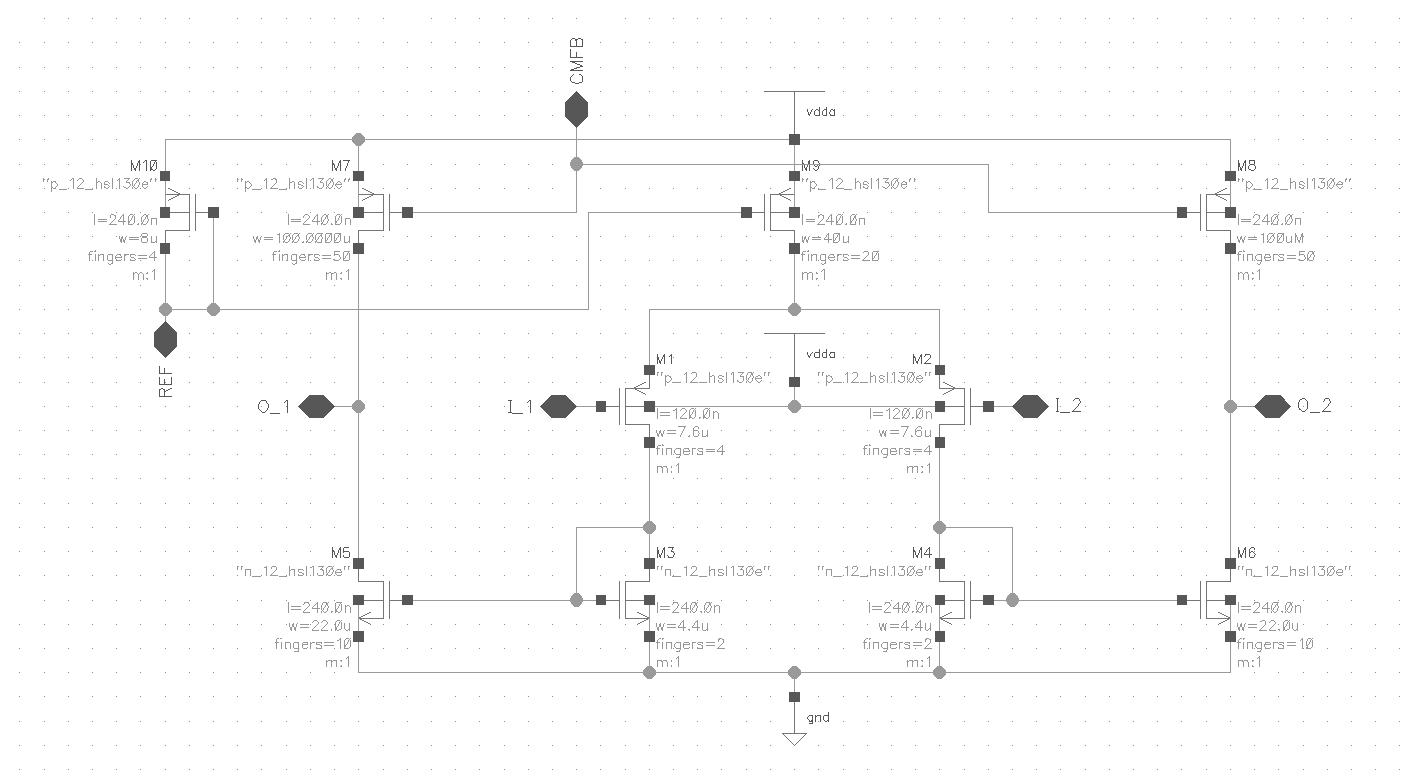
\includegraphics[width=1.0\linewidth]{imagespart2/schematics_OTA.png}
    \caption{Schematic}
\end{figure}
\begin{figure}[H]
    \centering
    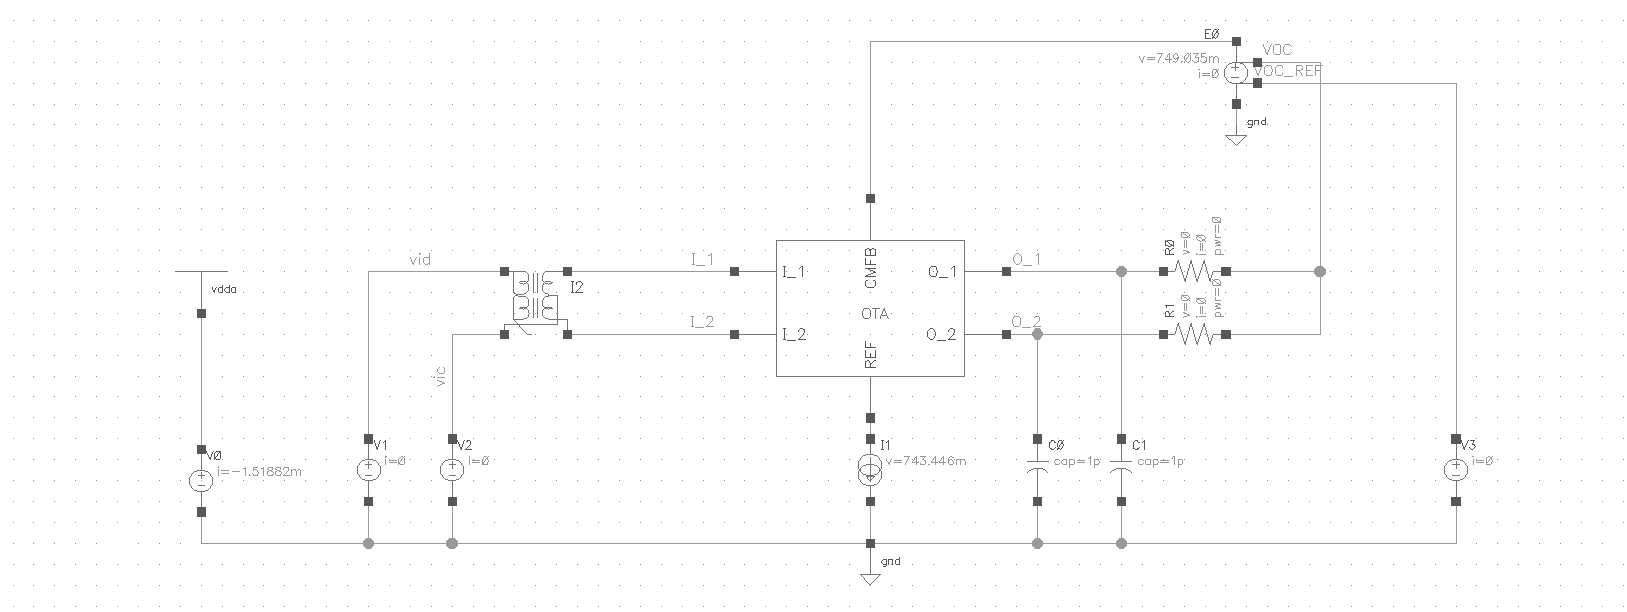
\includegraphics[width=1.0\linewidth]{imagespart2/schematics_tb.png}
    \caption{Testbench}
\end{figure}
\section{DC and Small-Signal Characterization}
\subsection{DC analysis}
\begin{figure}[H]
    \centering
    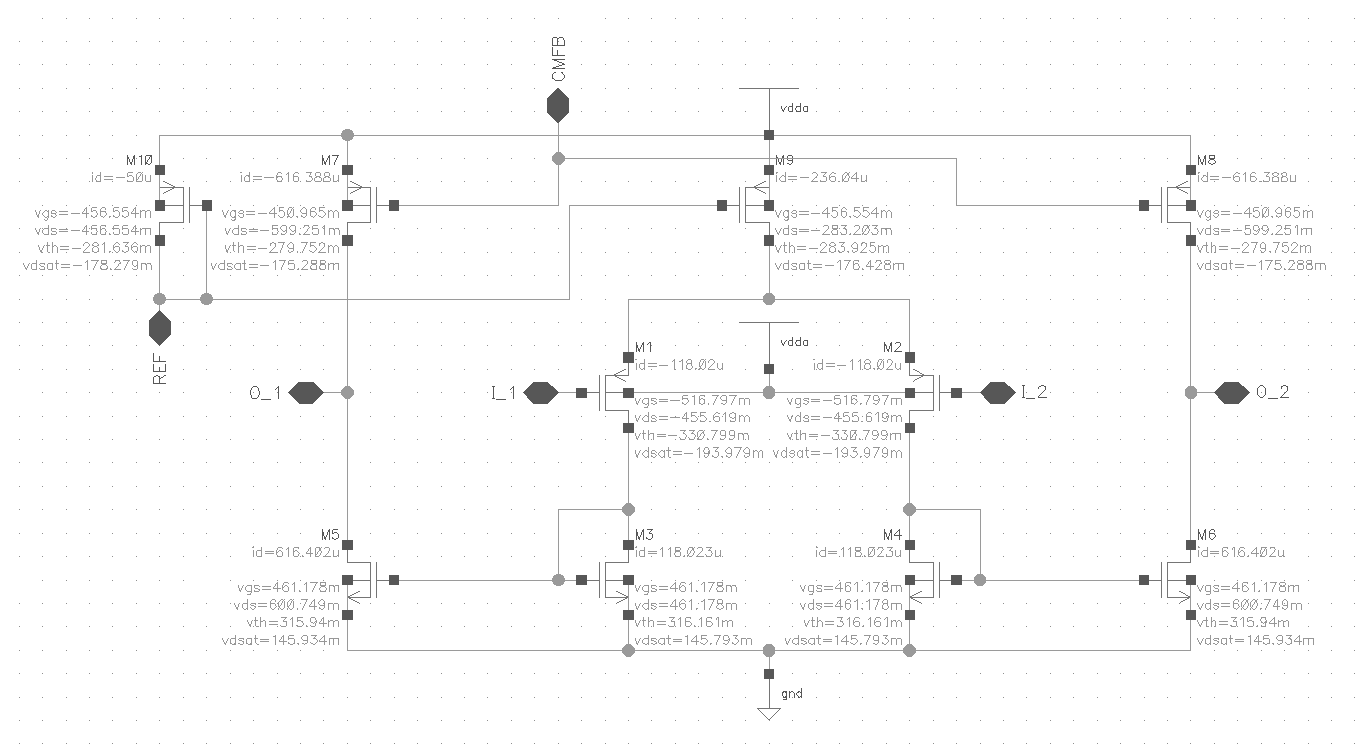
\includegraphics[width=1.0\linewidth]{imagespart2/OTA_OP.png}
    \caption{DC operating point}
\end{figure}


\begin{table}[H]
\centering
\caption{DC Operating Point Parameters of the OTA (Left Half-Circuit)}
\label{table:ota_op}
\begin{tabular}{|l|c|c|c|c|}
\hline
\textbf{Transistor} & \textbf{$|I_D|$ [$\mu$A]} & \textbf{$V_{DS}$ [mV]} & \textbf{$g_m$ [mS]} & \textbf{$r_o$ [k$\Omega$]} \\ \hline
M1  & 118.02  & 455.62 & 1.080   & 8.626  \\ \hline
M3  & 118.02 & 461.18 & 1.237 & 25.50 \\ \hline
M5  & 616.40 & 600.75 & 6.395 & 5.471  \\ \hline
M7  & 616.38 & 599.25 & 6.151 & 5.663 \\ \hline
M9  & 236.04 & 283.20 & 2.327 & 10.02   \\ \hline
M10 & 50 & 456.55 & 0.490 & 67.44 \\ \hline
\end{tabular}
\end{table}

\begin{figure}[H]
    \centering
    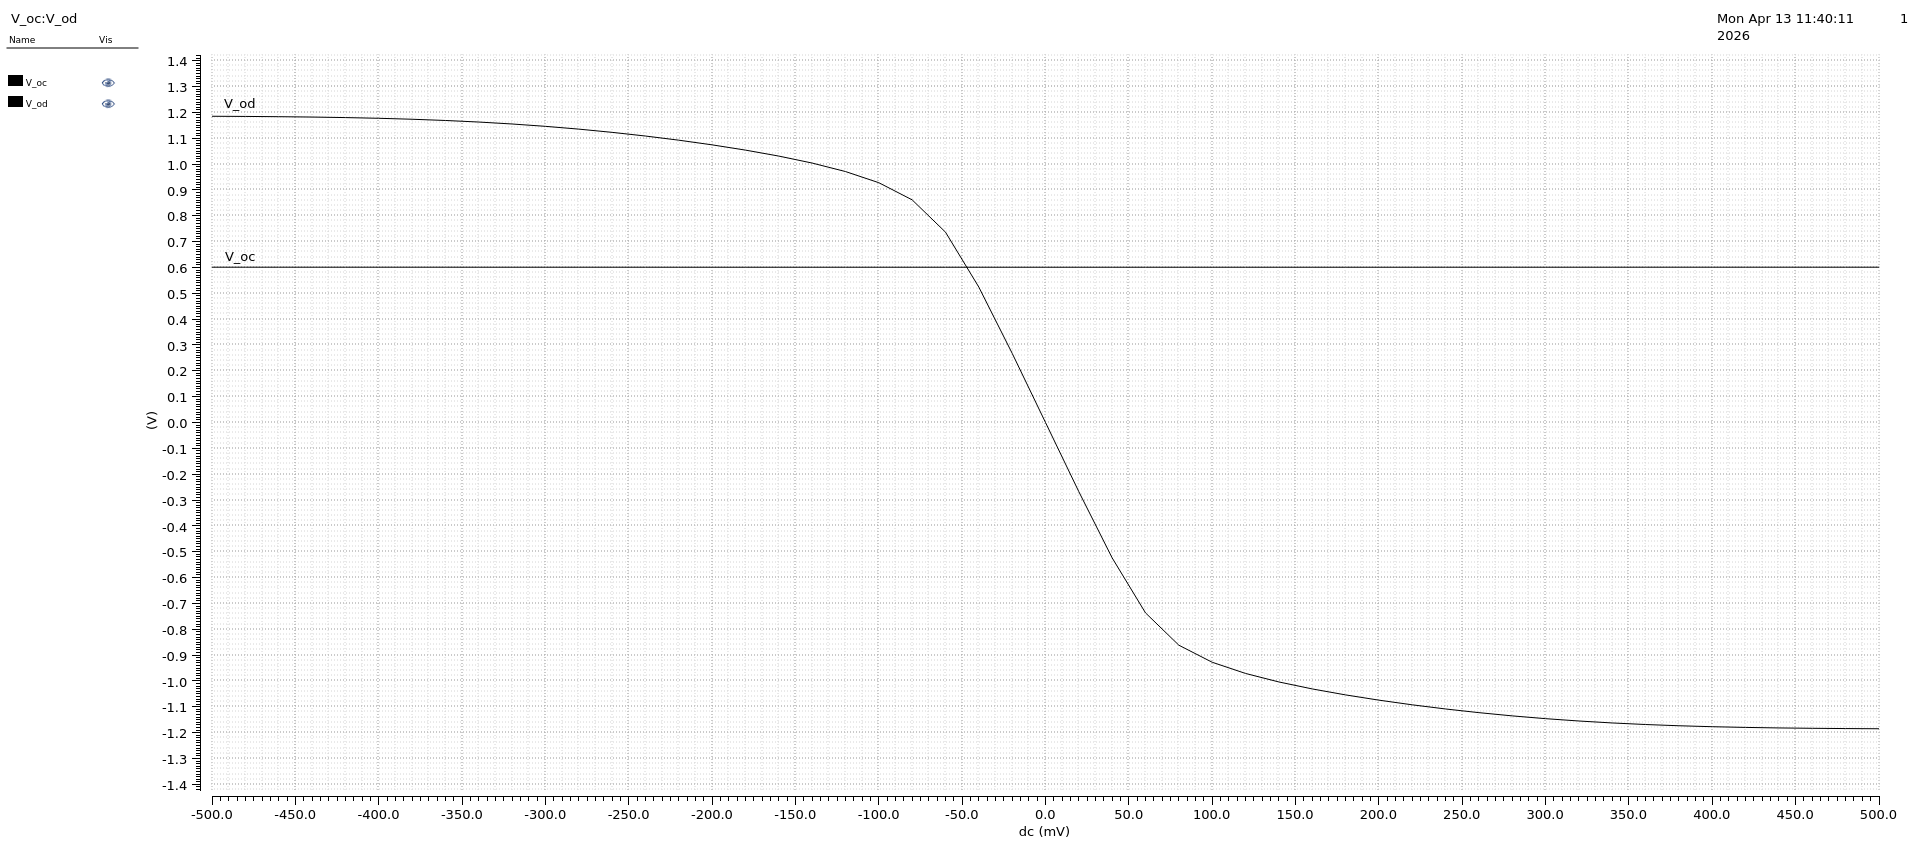
\includegraphics[width=1.0\linewidth]{imagespart2/V_oc_v_Vod.png}
    \caption{Differential output voltage $V_{OD}$ and common-mode output voltage $V_{OC}$ as functions of the differential input voltage $V_{ID}$.}
\end{figure}
\begin{figure}[H]
    \centering
    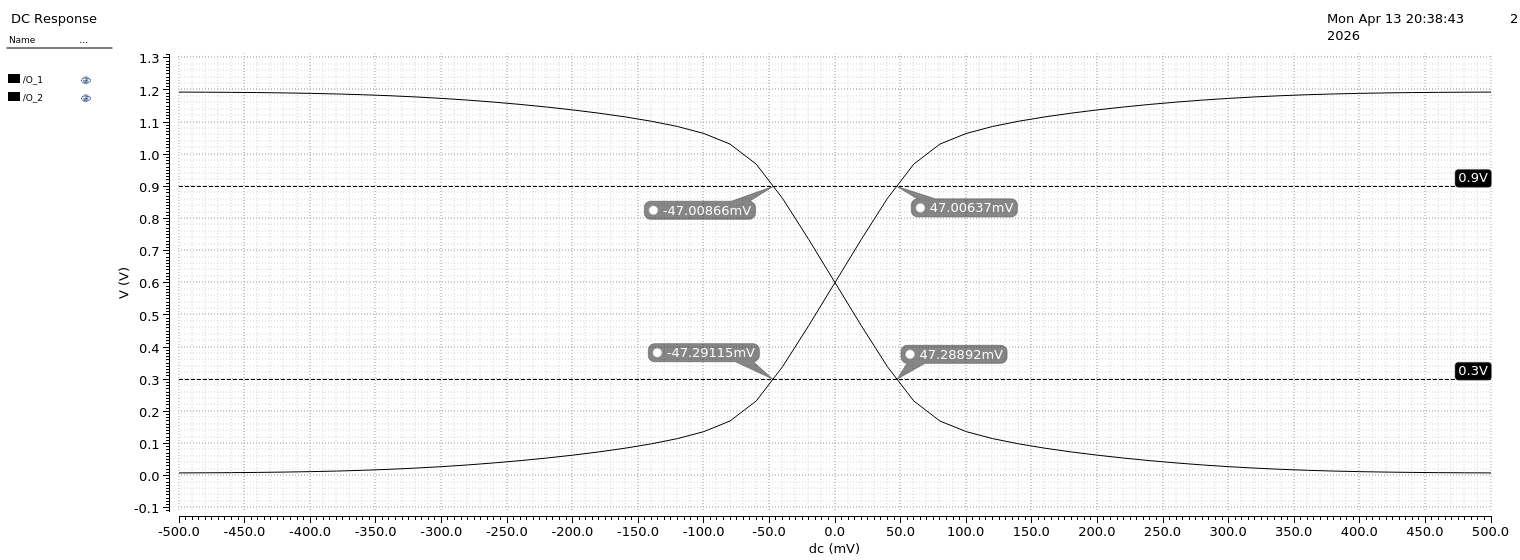
\includegraphics[width=1.0\linewidth]{imagespart2/Vo1_o2_id.png}
    \caption{Voltage outputs $V_{O1}$,$V_{O2}$ as functions $V_{ID}$.}
\end{figure}
\begin{figure}[H]
    \centering
    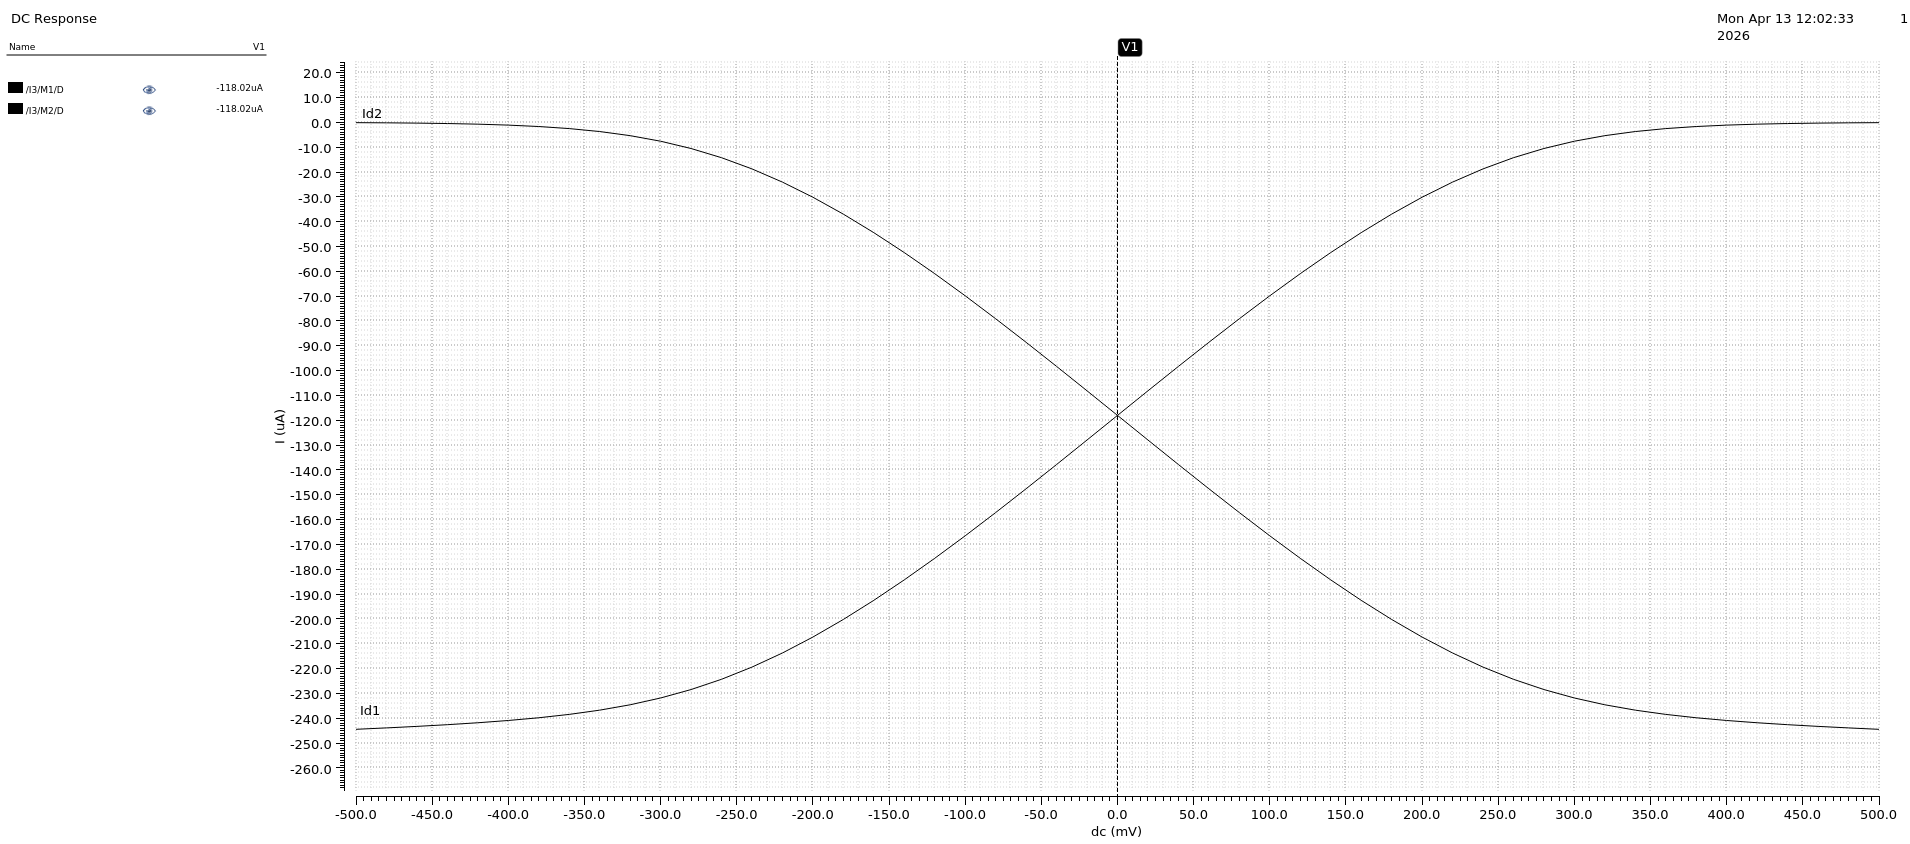
\includegraphics[width=1.0\linewidth]{imagespart2/Id1vId2.png}
    \caption{Differential pair currents as a function of $V_{ID}$.}
\end{figure}

\paragraph{Discussion of the differential-pair currents}
The simulated drain currents of the differential pair exhibit the expected current-steering behaviour. For large negative values of $V_{ID}$, most of the tail current flows through transistor M1, while the current in M2 becomes very small. Conversely, for large positive values of $V_{ID}$, the current is steered towards M2 and M1 is progressively turned off. Around $V_{ID}=0$, the two transistors conduct approximately the same current, corresponding to the balanced operating condition of the OTA.
\subsection{Differential mode ac analysis}
\begin{figure}[H]
    \centering
    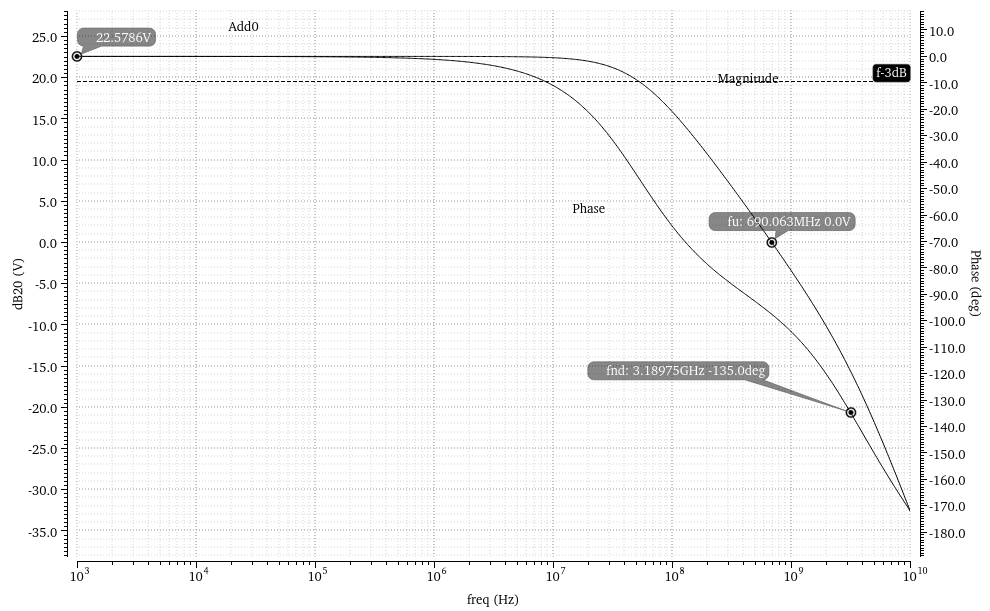
\includegraphics[width=1.0\linewidth]{imagespart2/differential_gain (1).png}
    \caption{Bode plot of magnitude and phase of the differential output voltage.}
\end{figure}


The differential-mode Bode plot has been analyzed by placing markers on both the magnitude and phase responses in order to extract the main performance parameters of the OTA. In particular, the low-frequency gain $A_{dd0}$, the $-3$ dB bandwidth $f_{-3\mathrm{dB}}$, and the unity-gain frequency $f_u$ have been identified from the magnitude response.

The extracted values are:

\begin{itemize}
    \item $A_{dd0}=22.58\,\mathrm{dB}$
    \item $f_{-3\mathrm{dB}}=52.28\,\mathrm{MHz}$
    \item $f_u=690.06\,\mathrm{MHz}$
\end{itemize}

The $-3$ dB bandwidth provides a good approximation of the dominant pole frequency:
\[
f_{dp}\approx f_{-3\mathrm{dB}}=52.28\,\mathrm{MHz}.
\]
Since the phase margin is large and the first non-dominant pole is located well above the unity-gain frequency, the gain-bandwidth product can be approximated as
\[
\mathrm{GBW}\approx f_u=690.06\,\mathrm{MHz}.
\]
The frequency of the first non-dominant pole was estimated from the phase response. A marker was placed at the frequency where the phase reaches approximately $-135^\circ$, corresponding to the point at which the second pole starts contributing significantly to the overall phase shift. This gives
\[
f_{nd}\approx 3.19\,\mathrm{GHz}.
\]
Since $f_{nd}\approx 4.6\,f_u$, the first non-dominant pole is sufficiently separated from the unity-gain frequency, confirming that the OTA behaves predominantly as a single-pole system around $f_u$.
\subsection{Common mode ac analysis}
\paragraph{Explanation for the very low value of the low-frequency
common-mode gain (and thus, very high CMRR)}
\begin{figure}[H]
    \centering
    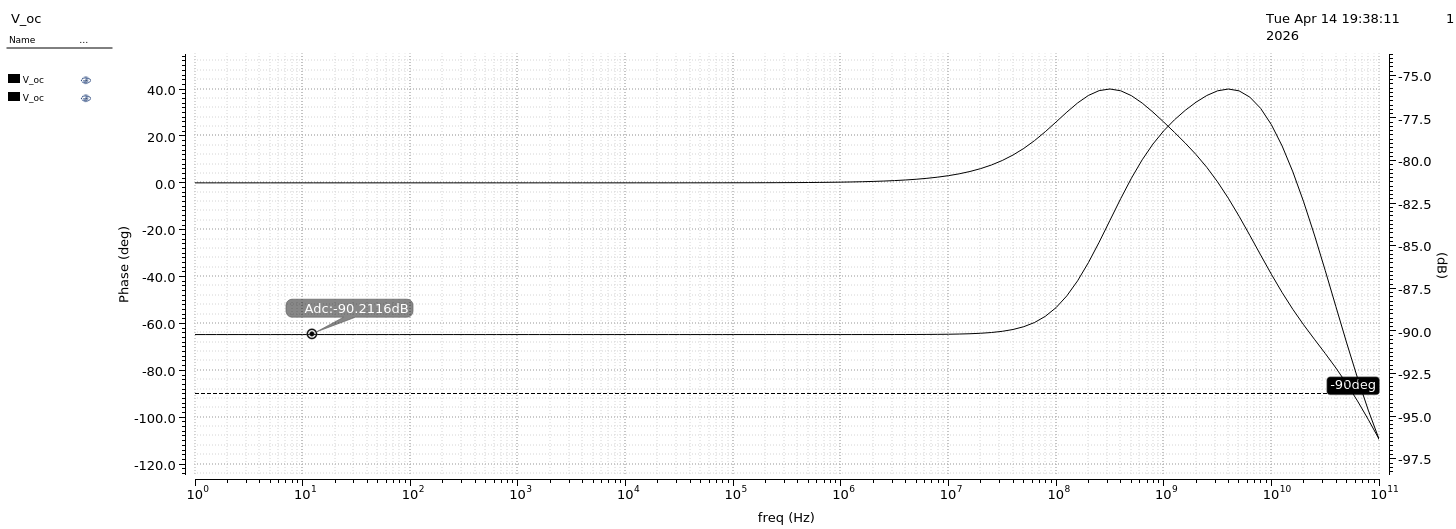
\includegraphics[width=1.0\linewidth]{imagespart2/Voc_gian_pahae.png}
    \caption{Bode plot of magnitude and phase of the common mode output voltage.}
\end{figure}
\paragraph{Discussion:}
The very low common-mode gain at low frequency is mainly due to the action of the Common-Mode Feedback (CMFB) loop. The CMFB senses the output common-mode voltage 
\[
V_{OC}=\frac{V_{O1}+V_{O2}}{2}
\]
and compares it with a reference value \(V_{OC,ref}\). Any deviation generates an error signal that is amplified and fed back to control the biasing of the output stage.

At low frequency, the CMFB loop has high gain, so it effectively forces
\[
V_{OC} \approx V_{OC,ref}
\]
independently of common-mode disturbances. As a result, variations in the input common-mode voltage produce only very small variations at the output, leading to a very low common-mode gain, and thus leading to a high CMRR.

\section{Estimation of the OTA Offset Voltage with a Monte Carlo Mismatch Simulation}


\begin{figure}[H]
    \centering
    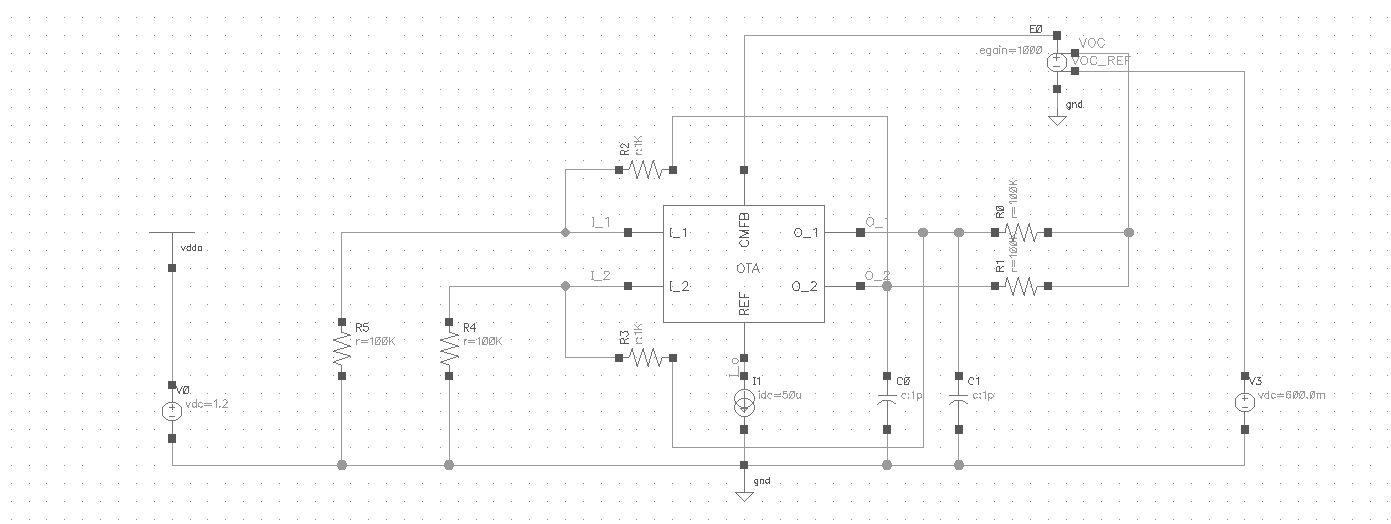
\includegraphics[width=1.0\textwidth]{imagespart2/ota_mirror_tb_schematic.png}
    \caption{Testbench used for the estimation of the OTA offset voltage.}
    \label{fig:vos_testbench}
\end{figure}
The OTA offset voltage was estimated by means of a Monte Carlo mismatch simulation including 100 runs. Using the feedback network shown in Fig.~\ref{fig:vos_testbench} and assuming $\beta A_{dd0} \gg 1$, the differential input voltage required to balance the output provides a good approximation of the input-referred mismatch voltage. Therefore, the OTA offset voltage can be estimated as

\[
V_{OS} \approx \sigma(V_{ID}).
\]

The distribution of $V_{ID}$ obtained from the Monte Carlo analysis is shown in Fig.~\ref{fig:hist_vid}. From the statistical data, the following standard deviation was extracted:

\[
\sigma(V_{ID}) =V_{OS}= 7.28\,\mathrm{mV}.
\]


\begin{figure}[H]
    \centering
    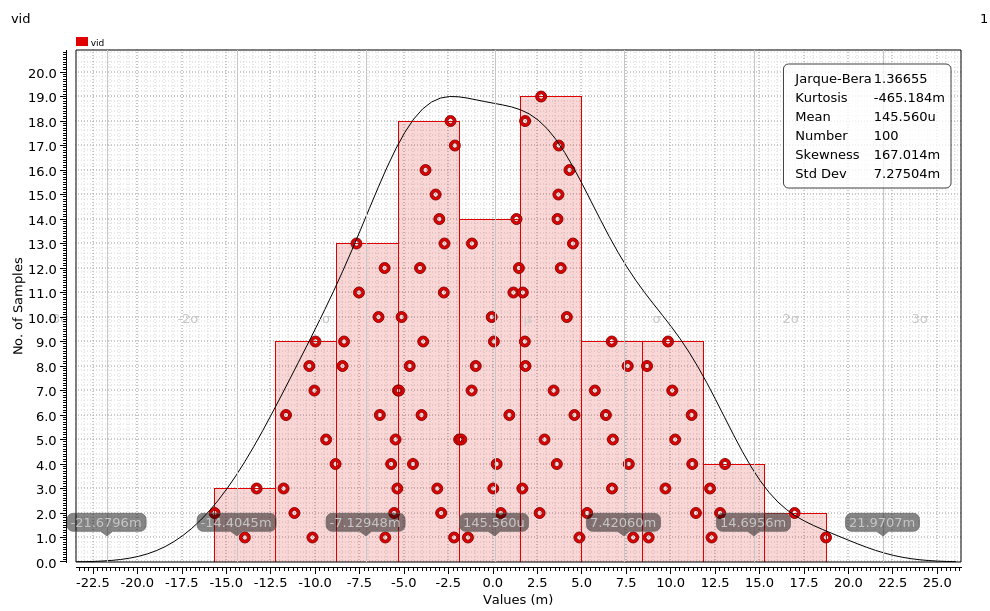
\includegraphics[width=1.0\textwidth]{imagespart2/Montecarlo Vid.png}
    \caption{Monte Carlo distribution of the differential input voltage $V_{ID}$.}
    \label{fig:hist_vid}
\end{figure}

\begin{figure}[H]
    \centering
    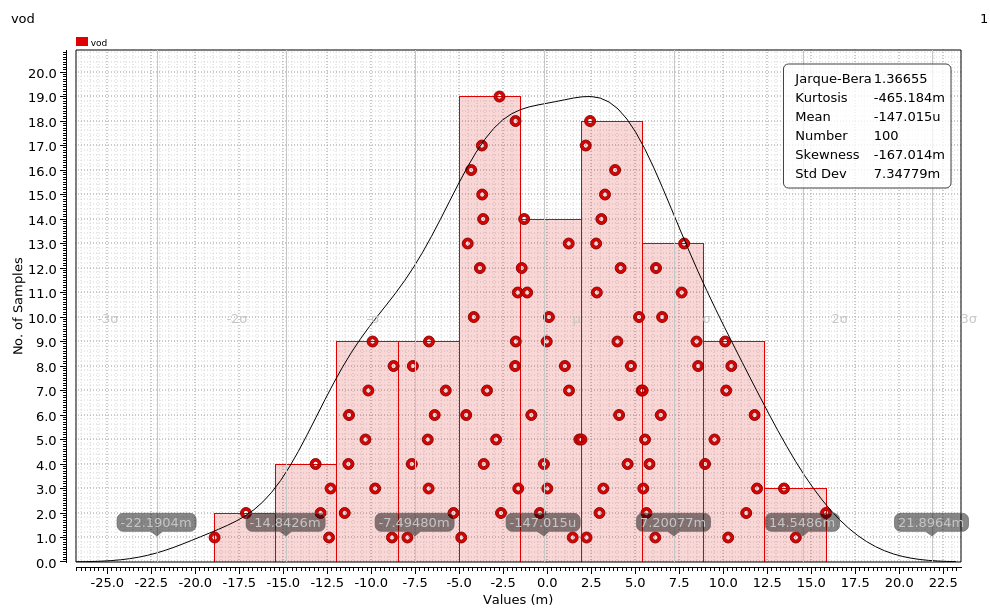
\includegraphics[width=1.0\textwidth]{imagespart2/Montecarlo Vod.png}
    \caption{Monte Carlo distribution of the differential output voltage $V_{OD}$.}
    \label{fig:hist_vod}
\end{figure}
\section{Redesign of the OTA to meet specifications}
The OTA was initially designed following the procedure described in the previous sections, targeting a gain-bandwidth product of $1\,\mathrm{GHz}$. However, AC simulations yielded a unity-gain frequency of approximately $600\,\mathrm{MHz}$, indicating that the simplified long-channel design equations overestimated the achievable performance.

To compensate for these non-ideal effects, the same sizing procedure was repeated using a more conservative target value

\[
GBW_{target}=1.6\,\mathrm{GHz}.
\]

This led to the following design parameters:

\[
G_m \approx 10.05\,\mathrm{mS},
\qquad
R_o \approx 3.96\,\mathrm{k}\Omega,
\]
with bias currents
\[
I_{D1}=I_{D2}\approx188\,\mu\mathrm{A},
\qquad
I_{B1}\approx376\,\mu\mathrm{A},
\qquad
I_{B2}\approx752\,\mu\mathrm{A}.
\]

The corresponding transistor dimensions were then calculated according to the adopted design methodology. In particular, the input differential pair dimensions were initially obtained as

\[
W_1=W_2=20\,\mu\mathrm{m},
\qquad
L_1=L_2=120\,\mathrm{nm}.
\]

Although this redesigned OTA exhibited a significant improvement with respect to the initial implementation, the simulated gain-bandwidth product was still slightly below the required specification of $1\,\mathrm{GHz}$.

Therefore, a final optimization step was performed by increasing the width of the input differential pair transistors from $20\,\mu\mathrm{m}$ to $33\,\mu\mathrm{m}$. This modification increases the transconductance $g_{m1}$ of the input stage by reducing its overdrive voltage, while still keeping the devices in strong inversion. As a consequence, the gain-bandwidth product is increased without significantly altering the bias currents, output resistance, or operating point of the OTA.

The final transistor dimensions adopted for the implementation are summarized in Table~\ref{tab:final_sizing2}.

\begin{table}[H]
\centering
\caption{Final transistor dimensions after optimization.}
\label{tab:final_sizing2}

\begin{tabular}{|c|c|c|}
\hline
\textbf{Transistor} & \textbf{W [$\mu$m]} & \textbf{L [nm]} \\ \hline
M1, M2 & $20 \xrightarrow{} 33$ & 120 \\ \hline
M3, M4 & 3.6 & 450 \\ \hline
M5, M6 & 14.4 & 450 \\ \hline
M7, M8 & 52 & 450 \\ \hline
M9 & 26 & 450 \\ \hline
M10 & 3.6 & 450 \\ \hline
\end{tabular}

\end{table}
\section{Final Design Verification}

\begin{figure}[H]
    \centering
    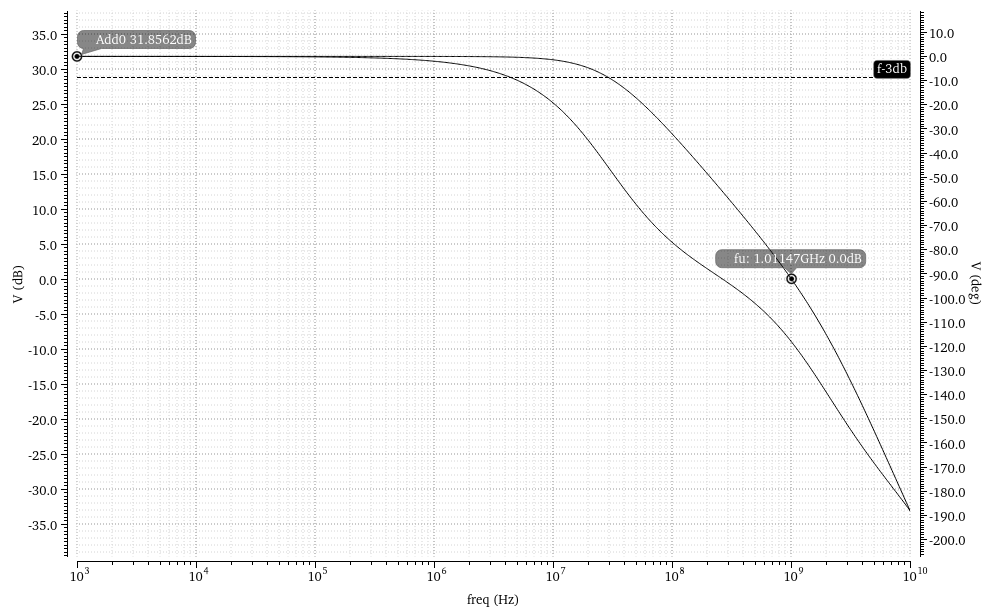
\includegraphics[width=\linewidth]{imagespart2/final_differential_gain.png}
    \caption{Differential-mode Bode plot of the final OTA design.}
    \label{fig:final_bode}
\end{figure}

The performance of the optimized OTA was verified through AC analysis. The differential-mode Bode plot reported in Fig.~\ref{fig:final_bode} shows that the final design successfully meets the assigned gain and bandwidth specifications.

The extracted values are:

\begin{itemize}
    \item $A_{dd0} \approx 31.86\,\mathrm{dB}$
    \item $GBW \approx 1.01\,\mathrm{GHz}$
\end{itemize}

The low-frequency gain exceeds the required specification of $30\,\mathrm{dB}$, while the unity-gain frequency is slightly above the target value of $1\,\mathrm{GHz}$. The increase of the input-pair width successfully enhanced the transconductance of the OTA, resulting in the desired improvement of the gain-bandwidth product without compromising the stability of the circuit.

\begin{figure}[H]
    \centering
    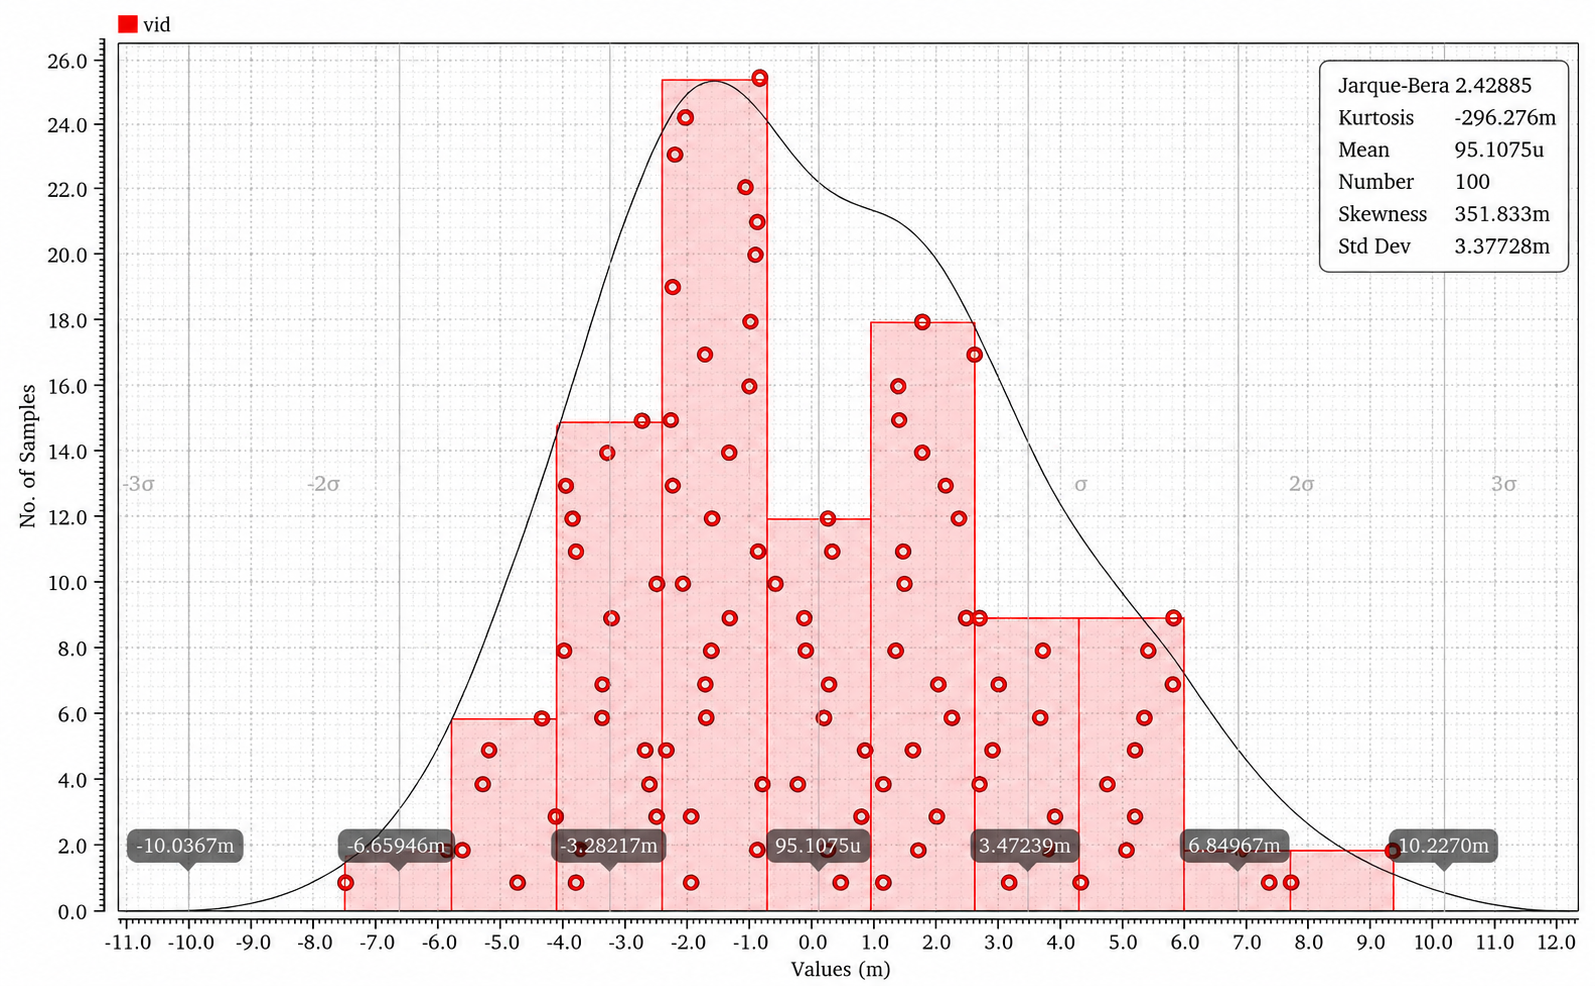
\includegraphics[width=\linewidth]{imagespart2/final_montecarlo_corretta.png}
    \caption{Monte Carlo distribution of the input-referred differential voltage $V_{ID}$ for the final OTA design.}
    \label{fig:final_mc}
\end{figure}

To verify the offset-voltage specification, a Monte Carlo mismatch simulation with $N=100$ runs was performed. The resulting distribution of the differential input voltage required to balance the output is shown in Fig.~\ref{fig:final_mc}.

From the statistical analysis, the standard deviation of the distribution was found to be

\[
\sigma(V_{ID}) =V_{OS}= 3.38\,\mathrm{mV}.
\]
\begin{table}[H]
\centering
\caption{Final specification verification.}
\label{tab:final_results}

\begin{tabular}{|c|c|c|c|}
\hline
\textbf{Parameter} & \textbf{Specification} & \textbf{Simulated} \\ \hline
$A_{dd0}$ & $>30\,\mathrm{dB}$ & $31.86\,\mathrm{dB}$  \\ \hline
GBW & $\geq1\,\mathrm{GHz}$ & $1.01\,\mathrm{GHz}$  \\ \hline
$V_{OS}$ & $<4\,\mathrm{mV}$ & $3.38\,\mathrm{mV}$  \\ \hline
\end{tabular}

\end{table}


\chapter{LAB Session 03 --Capacitive feedback amplifier
based on a two-stage OTA}
\section{Initial design analysis}

\subsection{Initial transistors and DC Operating Point Verification}
% subsection was incorrect.
\begin{table}[h]
\centering
\begin{tabular}{|c|c|c|c|c|c|}
\hline
\textbf{Transistor} &
\textbf{$|V_{OV}|$ [V]} &
\textbf{L [$\mu$m]} &
\textbf{W [$\mu$m]} &
\textbf{\# Fingers} &
\textbf{$I_D$ [$\mu$A]}
\\ \hline

M1, M2 &
0.14 &
0.24 &
4 &
4 &
100.2
\\ \hline

M3, M4 &
0.21 &
0.24 &
12 &
8 &
100.2
\\ \hline

M5, M6 &
0.22 &
0.24 &
48 &
24 &
444.2
\\ \hline

M7, M8 &
0.13 &
0.24 &
19.2 &
16 &
444.2
\\ \hline

M9A, M9B &
0.13 &
0.24 &
4.8 &
4 &
100.2
\\ \hline

M10, M11 &
0.21 &
0.24 &
6 &
4 &
53.56
\\ \hline

M12 &
0.13 &
0.24 &
2.4 &
2 &
53.56
\\ \hline

\end{tabular}
\caption{Initial transistor sizing of the fully differential two-stage OTA.}
\label{tab:ota_initial_sizing}
\end{table}


\begin{figure}[H]
    \centering
    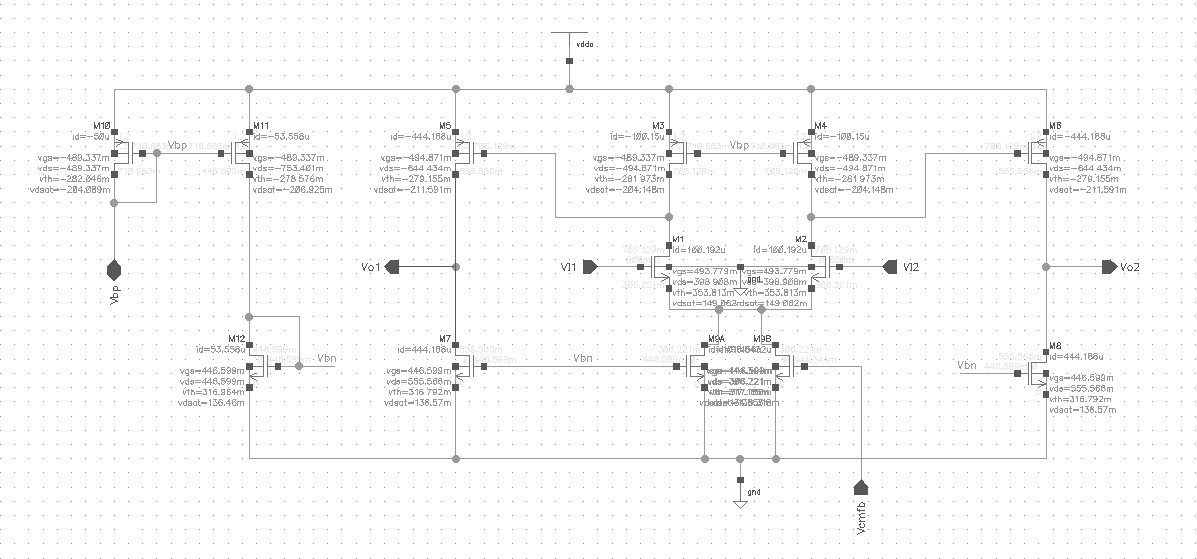
\includegraphics[width=1.0\textwidth]{Images_part3/TS_OTA_OL_OP.png}
    \caption{DC operating point of the initial OTA design.}
    \label{fig:initial_ota_operating_point}
\end{figure}
The operating point simulation confirms that all transistors are correctly biased in saturation region. Moreover, the common-mode output voltage settles close to the desired value, indicating a correct operation of the common-mode feedback network.
\subsection{Open-Loop OTA Analysis}
\begin{figure}[H]
    \centering
    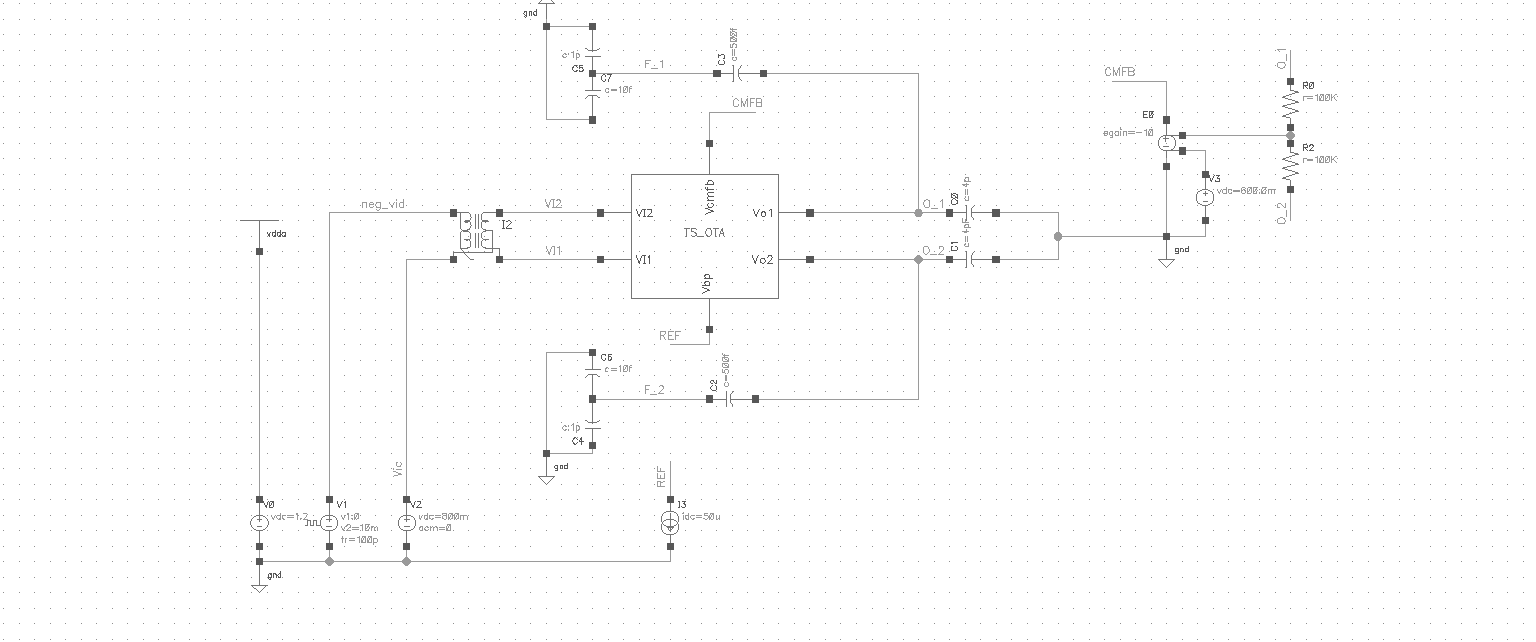
\includegraphics[width=1.0\textwidth]{Images_part3/OL_TESTBENCH.png}
    \caption{Open-loop testbench used for loop transfer function characterization.}
    \label{fig:tb_ol}
\end{figure}
The open-loop characterization of the OTA was performed using the testbench shown in Fig.~\ref{fig:tb_ol}. The capacitive feedback network was disconnected from the OTA input in order to evaluate the loop transfer function and assess the intrinsic stability of the amplifier.
The feedback factor
\[
\beta=\frac{C_F}{C_F+C_S+C_I}\approx0.33
\]
represents the fraction of the output signal fed back to the OTA input through the capacitive network. It therefore determines the loop transfer function
\[
T(s)=\beta A_{OL}(s),
\]
and directly affects the stability and phase margin of the closed-loop system. $A_{OL}(s)$ is the open-loop differential gain of the OTA. Using this setup, the Bode plots and transient responses reported in the following section were extracted.


\begin{figure}[H]
    \centering
    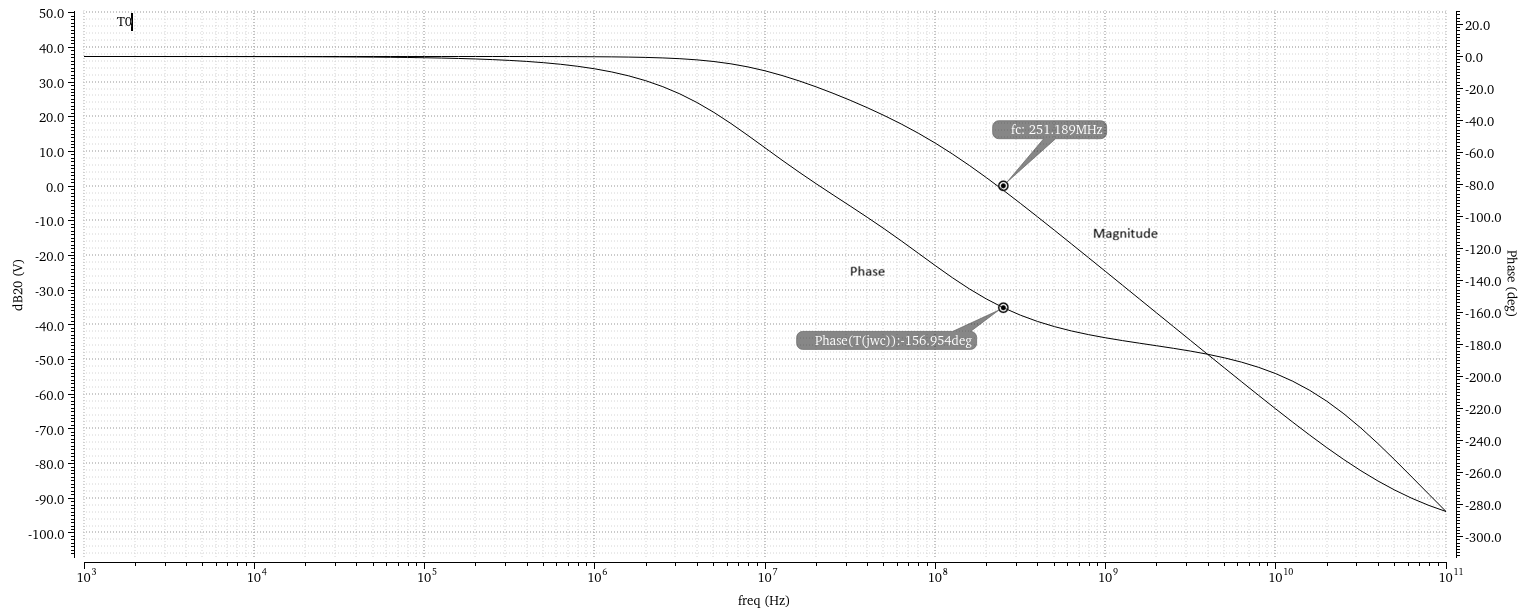
\includegraphics[width=1.0\textwidth]{Images_part3/T0_bodeplt.png}
    \caption{Bode plot of the open-loop transfer function.}
    \label{fig:open_loop_bode}
\end{figure}
The initial loop transfer function exhibits a low-frequency gain of $T_0\approx37.8\,\mathrm{dB}$, a crossover frequency of $f_c\approx251\,\mathrm{MHz}$, and a phase margin of only $PM\approx23^\circ$. Although the bandwidth is relatively high, the poor phase margin indicates insufficient stability and makes the circuit unsuitable for closed-loop operation. Therefore, frequency compensation is required.
\subsection{Transient response of the differential and common mode signal}


\begin{figure}[H]
    \centering
    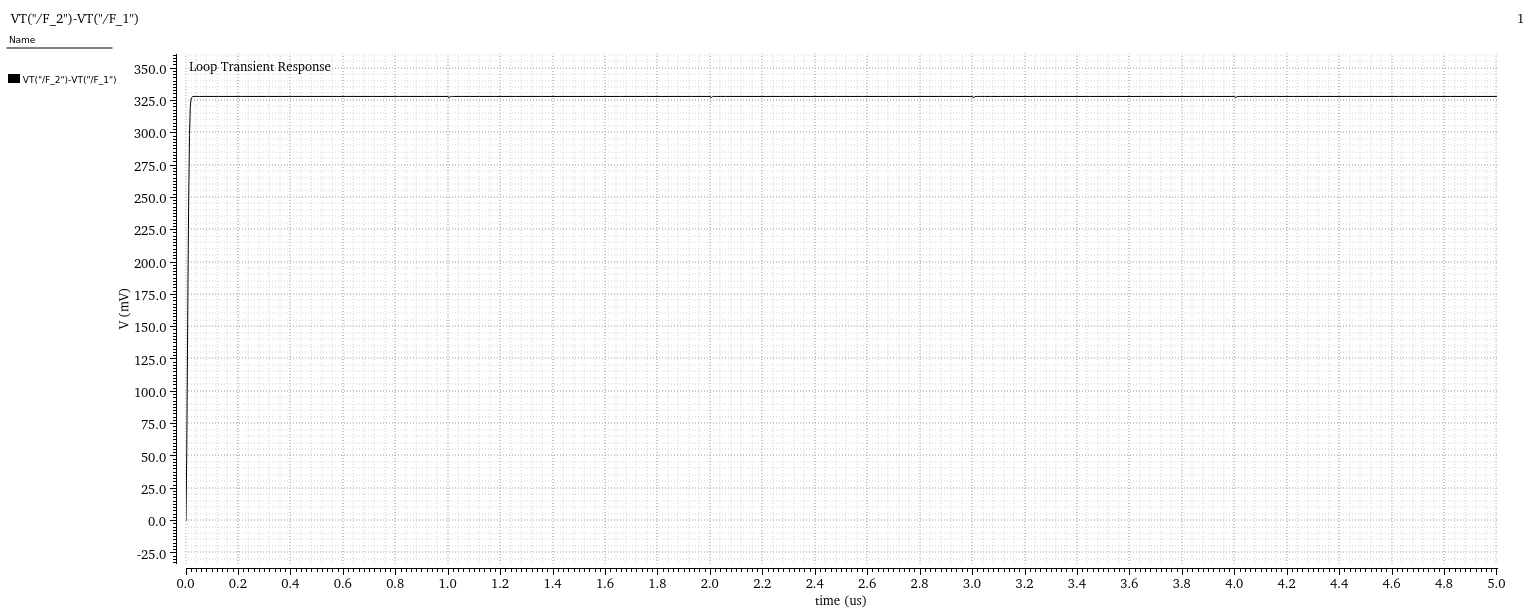
\includegraphics[width=1.0\textwidth]{Images_part3/loop_tran_resp.png}
    \caption{Transient response of the loop differential output signal.}
    \label{fig:open_loop_transient}
\end{figure}
The differential transient response confirms the high gain and bandwidth of the uncompensated OTA. A small differential input step produces a large output variation, consistent with the large open-loop gain previously observed in the frequency-domain analysis.


\begin{figure}[H]
    \centering
    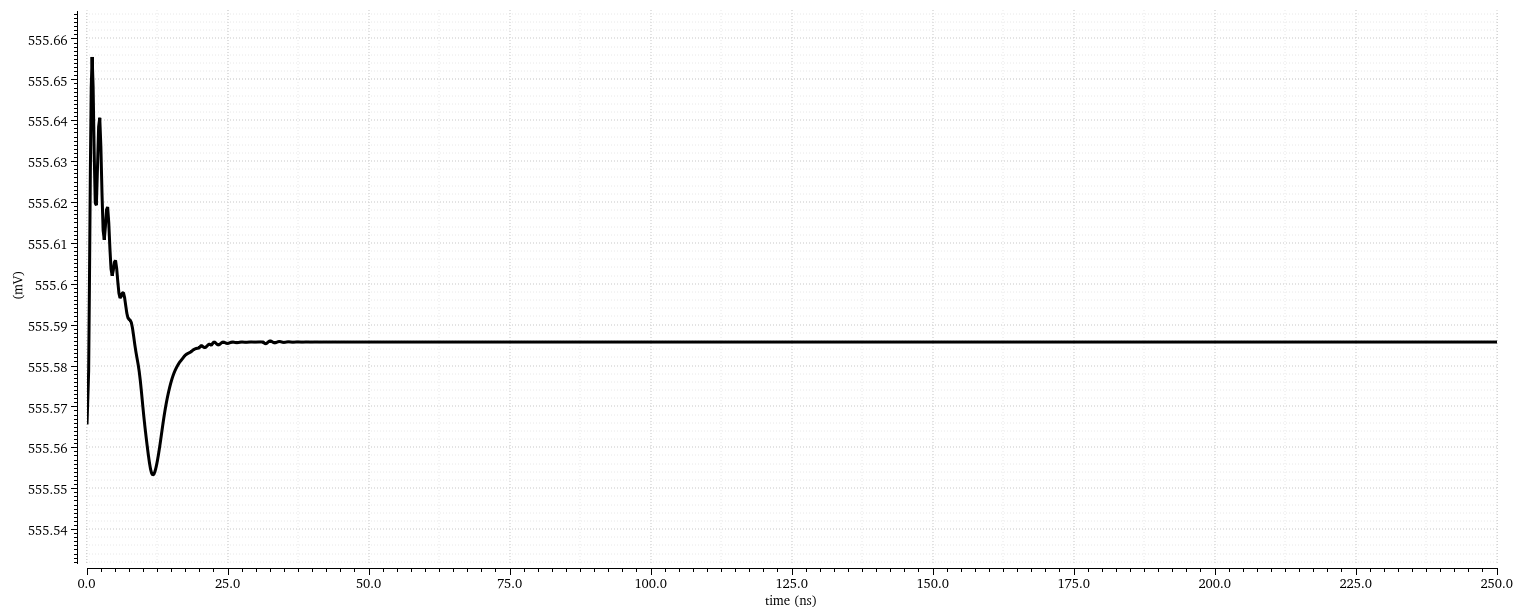
\includegraphics[width=1.0\textwidth]{Images_part3/OL_tran_cm.png}
    \caption{Transient response of the loop common-mode output component.}
    \label{fig:open_loop_common_mode_transient}
\end{figure}
The common-mode transient response confirms effective CMFB loop operation. After a minimal overshoot of $\Delta V_{OCM}\approx 0.1\,\mathrm{mV}$, the output common-mode voltage rapidly settles to $V_{OCM}\approx 556\,\mathrm{mV}$, demonstrating stable regulation and precise control of the common-mode level.

\subsection{Closed-Loop Feedback Amplifier Analysis}

\begin{figure}[H]
    \centering
    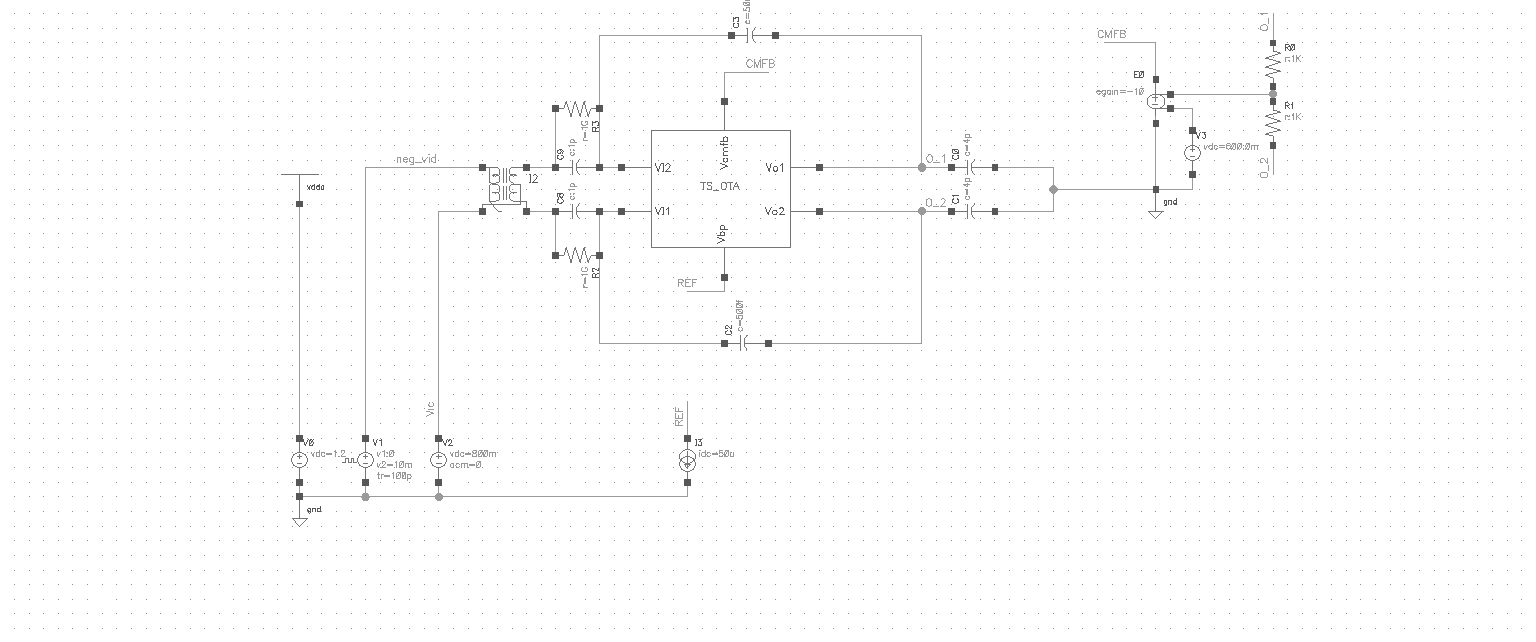
\includegraphics[width=1.0\textwidth]{Images_part3/cl3_TESTBENCH.png}
    \caption{Closed-loop testbench used for capacitive feedback amplifier characterization.}
    \label{fig:tb_cl}
\end{figure}
The closed-loop behavior of the capacitive feedback amplifier was analyzed using the testbench shown in Fig.~\ref{fig:tb_cl}. In this configuration, the capacitive feedback network is connected around the OTA, thus establishing the differential closed-loop gain through the capacitor ratio.

Assuming an ideal OTA with sufficiently large loop gain, the low-frequency closed-loop gain is

\[
A_{CL,\mathrm{ideal}}
=
-\frac{C_S}{C_F}
=
-2.
\]
The large input resistors are used to impose the input common-mode voltage without significantly affecting the ac response of the capacitive network. The testbench also includes the external load capacitances and the ideal common-mode feedback circuit in order to reproduce the intended operating conditions of the amplifier.

Using this setup, the closed-loop frequency response and transient step response of the feedback amplifier were extracted and analyzed.
\begin{figure}[H]
    \centering
    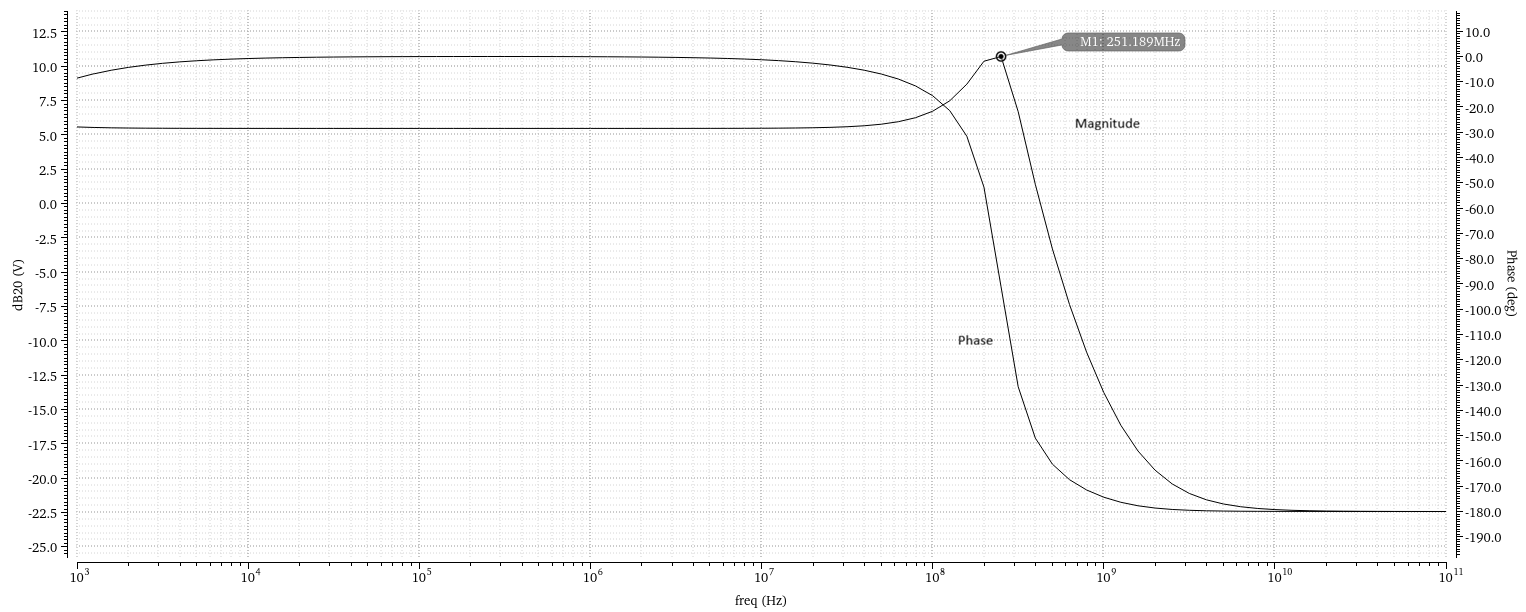
\includegraphics[width=1.0\textwidth]{Images_part3/CL_bodeplt.png}
    \caption{Bode plot of the closed-loop differential transfer function.}
    \label{fig:closed_loop_bode}
\end{figure}
The closed-loop differential transfer function exhibits a low-frequency gain of approximately

\[
A_{CL,0}\approx5.2\,\mathrm{dB},
\]

which is close to the ideal value expected from the capacitive feedback network.

However, a pronounced resonant peak is clearly visible around the bandwidth frequency, indicating a strongly underdamped closed-loop response. This behavior is consistent with the low phase margin previously extracted from the loop transfer function.


\subsection{Transient response of the differential mode signal}
\begin{figure}[H]
    \centering
    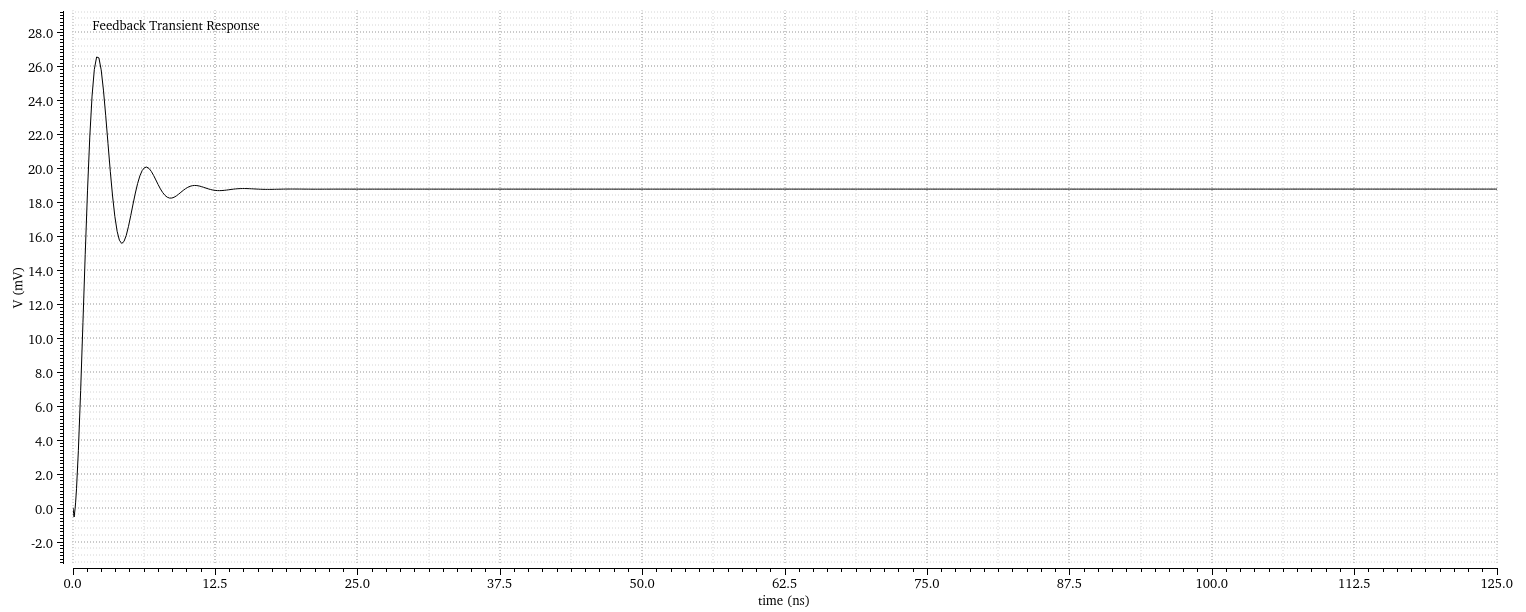
\includegraphics[width=1.0\textwidth]{Images_part3/Feed_tran_resp_doppia.png}
    \caption{Transient step response of the closed-loop differential output signal.}
    \label{fig:closed_loop_transient}
\end{figure}
The closed-loop differential step response confirms the poor stability predicted by the initial loop-transfer analysis ($PM \approx 23^\circ$). Consequently, the output exhibits severe ringing and a large overshoot, reaching a peak value of $v_{o,\mathrm{peak}} \approx 26.3\,\mathrm{mV}$ before settling toward a steady-state value of $v_o(\infty) \approx 18.9\,\mathrm{mV}$.



\section{OTA Redesign}
\subsection{First-Order Hand Design of the OTA}
The redesign process starts from the dynamic error specification. Assuming a first-order closed-loop response, the dynamic error is approximated as:
\begin{equation*}
\varepsilon_d(t_s)\simeq e^{-\omega_c t_s}
\end{equation*}
Imposing a settling error below $0.2\%$ after $20\,\mathrm{ns}$ yields:
\begin{align*}
\varepsilon_d(t_s) \leq 0.002 \implies \omega_c \geq \frac{-\ln(0.002)}{20\,\mathrm{ns}} \simeq 310\,\mathrm{Mrad/s} \implies f_c = \frac{\omega_c}{2\pi} \simeq 49.5\,\mathrm{MHz}
\end{align*}
Consequently, the OTA target crossover frequency is set to \boxed{f_c\simeq50\,\mathrm{MHz}}.

To satisfy the power constraint, the differential pair and second-stage transistors are biased at $I_{D1}=I_{D5}=225\,\mu\mathrm{A}$, with a total current consumption of:
\begin{equation*}
I_{TOT} = 2I_{REF}+2I_{D1}+2I_{D5} = 2\cdot50 + 2\cdot225 + 2\cdot225 = 1\,\mathrm{mA}
\end{equation*}
Overdrive voltages are chosen as $V_{OV1}=V_{OV5}=0.15\,\mathrm{V}$ and $V_{OV3}=V_{OV7}=V_{OV9}=V_{OV10}=V_{OV11}=V_{OV12}=0.3\,\mathrm{V}$. The resulting transconductance for the driving transistors is:
\begin{equation*}
g_{m1}=g_{m5} = \frac{2I_D}{V_{OV}} = \frac{2\cdot225\,\mu\mathrm{A}}{0.15\,\mathrm{V}} = 3\,\mathrm{mS}
\end{equation*}

The static error spec requires $\varepsilon_0 \simeq \frac{1}{1+T_0} \leq 0.002$, where $T_0=\beta A_{dd0}$ and $\beta=0.33$, hence $A_{dd0} \geq \frac{499}{0.33} \simeq 1512$. To ensure design margin, a larger open-loop gain target is adopted:
\begin{equation*}
A_{dd0} \simeq g_{m1}g_{m5}R_1R_2 \simeq 2025
\end{equation*}
Assuming $R_1=R_2=15\,\mathrm{k}\Omega$ (where $R_1=r_{o1}\parallel r_{o3}$ and $R_2=r_{o5}\parallel r_{o7}$), the estimated gain is verified:
\begin{equation*}
A_{dd0} = (3\,\mathrm{mS})^2 \cdot (15\,\mathrm{k}\Omega)^2 \simeq 2025
\end{equation*}
Assuming symmetric output resistances $r_{o1}=r_{o3}=r_{o5}=r_{o7}=30\,\mathrm{k}\Omega$, the channel lengths are estimated via $r_o=\frac{\eta L}{I_D} \implies L=\frac{r_o I_D}{\eta}$:
\begin{align*}
L_n &= \frac{30\,\mathrm{k}\Omega\cdot225\,\mu\mathrm{A}}{1.1\cdot10^7} \simeq 0.61\,\mu\mathrm{m} \implies L_1=L_7=L_9=L_{12}\simeq0.61\,\mu\mathrm{m} \\
L_p &= \frac{30\,\mathrm{k}\Omega\cdot225\,\mu\mathrm{A}}{1.5\cdot10^7} \simeq 0.45\,\mu\mathrm{m} \implies L_3=L_5=L_{10}=L_{11}\simeq0.45\,\mu\mathrm{m}
\end{align*}
Transistor widths are calculated using $W = \frac{2I_D L}{k'V_{OV}^2}$, matching the current-mirror ratios $\frac{W_3}{W_{10}} = \frac{W_7}{W_{12}} = \frac{225}{50} = 4.5$. The final hand-estimated dimensions are summarized in Table~\ref{tab:redesign_hand_sizing}.

\begin{table}[H]
\centering
\caption{Hand-estimated transistor dimensions for the redesigned OTA.}
\label{tab:redesign_hand_sizing}
\begin{tabular}{|c|c|c|c|c|}
\hline
\textbf{Transistor} & \textbf{$V_{OV}$ [V]} & \textbf{L [$\mu$m]} & \textbf{W [$\mu$m]} & \textbf{$I_D$ [$\mu$A]} \\ \hline
M1, M2 & 0.15 & 0.61 & 26.1 & 225 \\ \hline
M3, M4 & 0.30 & 0.45 & 22.5 & 225 \\ \hline
M5, M6 & 0.15 & 0.45 & 90.0 & 225 \\ \hline
M7, M8 & 0.30 & 0.61 & 6.53 & 225 \\ \hline
M9A, M9B & 0.30 & 0.61 & 6.53 & 225 \\ \hline
M10, M11 & 0.30 & 0.45 & 5.0 & 50 \\ \hline
M12 & 0.30 & 0.61 & 1.45 & 50 \\ \hline
\end{tabular}
\end{table}

Under dominant-pole conditions, the closed-loop bandwidth is $f_{BW,CL}\approx\beta\cdot GBW$, requiring a minimum $GBW \simeq \frac{50\,\mathrm{MHz}}{0.33} \simeq 150\,\mathrm{MHz}$. To account for non-idealities observed in previous iterations, a conservative target of $GBW\simeq300\,\mathrm{MHz}$ is chosen. The compensation capacitor is:
\begin{equation*}
GBW=\frac{g_{m1}}{2\pi C_C} \implies C_C = \frac{3\,\mathrm{mS}}{2\pi\cdot300\,\mathrm{MHz}} \simeq 1.6\,\mathrm{pF}
\end{equation*}
To improve the phase margin ($PM$), a nulling resistor $R_Z$ compensates the non-dominant pole:
\begin{equation*}
PM = 90.1^\circ - \tan^{-1}\left(\beta\frac{g_{m1}}{g_{m5}}\frac{C_L}{C_C}\right) + \tan^{-1}\left(\beta\frac{g_{m1}}{g_{m5}}k\right)
\end{equation*}
From this, the zero-position parameter is $k\simeq1.376$, yielding:
\begin{equation*}
R_Z = \frac{1+k}{g_{m5}} = \frac{1+1.376}{3\,\mathrm{mS}} \simeq 790\,\Omega \approx 800\,\Omega
\end{equation*}
These values served as the initial design point for subsequent Cadence simulations.

\subsection{Simulation-Based Optimization of the Initial OTA Design}

Although the analytical design satisfied first-order specifications, non-ideal effects neglected in the simplified hand calculations introduced discrepancies between theoretical predictions and simulated performance.

In the initial simulation iterations, the low-frequency gain was significantly lower than targeted. To counteract this, the channel lengths of the transistors dictating the gain of both stages (\(M_1\), \(M_3\), \(M_5\)) and the corresponding bias-current mirrors were progressively increased. This adjustment enhanced the equivalent output resistances:
\[
R_1=r_{o1}\parallel r_{o3}, \qquad R_2=r_{o5}\parallel r_{o7}
\]
Simultaneously, the transistor widths were rescaled to preserve the design overdrive voltages and bias currents.

Once the loop-gain target was secured, the optimization focused on the compensation network. The compensation capacitor \(C_C\) and the nulling resistor \(R_Z\) were iteratively tuned to suppress the phase degradation from non-dominant poles and maximize the phase margin. The final optimized compensation values are:
\[
\boxed{C_C=2.61\,\mathrm{pF}}, \qquad \boxed{R_Z=1.7\,\mathrm{k}\Omega}
\]

The final transistor dimensions and layout configurations resulting from the simulation-based refinement are summarized in Table~\ref{tab:final_ota_sizing4}.

\begin{table}[H]
\centering
\begin{tabular}{|c|c|c|}
\hline
\textbf{Transistor} & \textbf{L [$\mu$m]} & \textbf{W [$\mu$m]} \\ \hline
M1, M2    & 0.96 & 40.8  \\ \hline
M3, M4    & 1.2  & 60    \\ \hline
M5, M6    & 1.2  & 240   \\ \hline
M7, M8    & 0.96 & 10.2  \\ \hline
M9A, M9B & 0.96 & 10.2  \\ \hline
M10, M11 & 1.2  & 13.34 \\ \hline
M12       & 0.96 & 2.27  \\ \hline
\end{tabular}
\caption{Final optimized OTA transistor sizing after simulations.}
\label{tab:final_ota_sizing4}
\end{table}

\subsection{DC Operating Point Verification}
The final OTA DC operating point is reported in Fig.~\ref{fig:dc_op_point}. All transistors operate in saturation, validating the small-signal biasing conditions.

\begin{figure}[H]
    \centering
    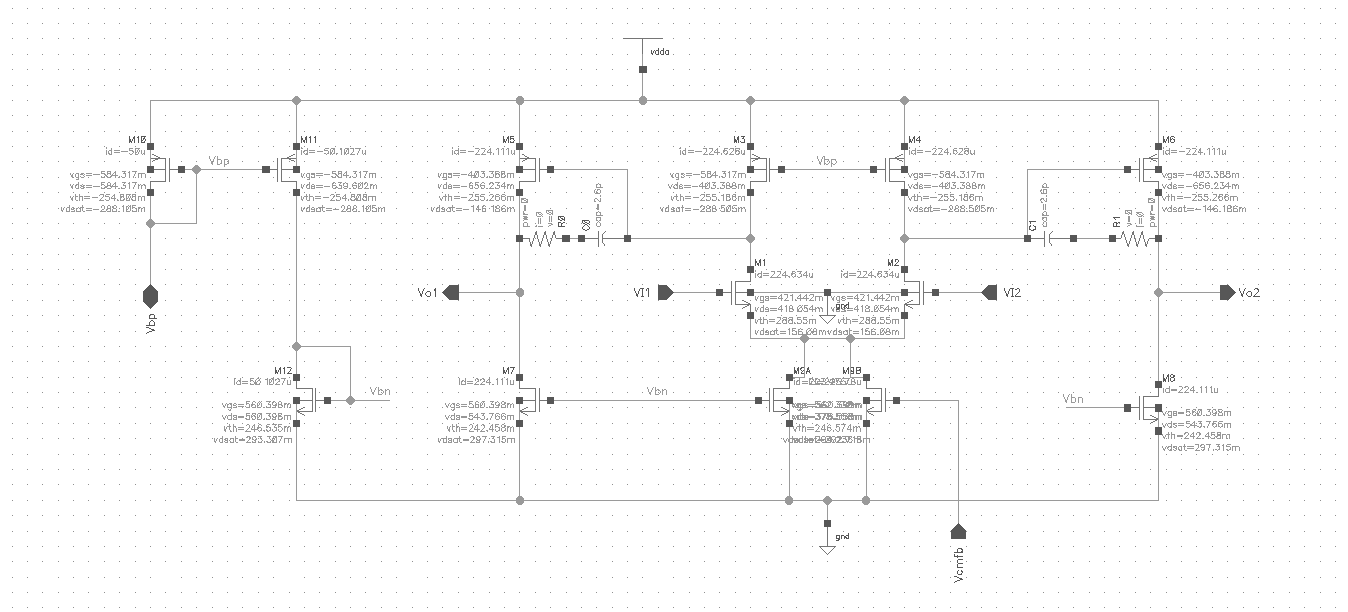
\includegraphics[width=0.9\textwidth]{immaginicorrettereport3/DC_OP_POINT.png}
    \caption{DC operating point of the final OTA design.}
    \label{fig:dc_op_point}
\end{figure}

The simulated branch currents are $I_D \simeq 224.6\,\mu\mathrm{A}$, $I_{D5}\simeq224.1\,\mu\mathrm{A}$, and $I_{REF}=50\,\mu\mathrm{A}$, yielding a total current consumption of:
\[
I_{TOT}=2I_{REF}+2I_D+2I_{D5} \simeq 997\,\mu\mathrm{A}
\]
This satisfies the power constraint $I_{TOT}<1\,\mathrm{mA}$. With $V_{DD}=1.2\,\mathrm{V}$, the resulting DC power consumption is:
\[
P_{DC}=V_{DD}I_{TOT} \simeq 1.20\,\mathrm{mW}
\]

\subsection{Loop Transfer Function Analysis}

The Bode plot of the loop transfer function (Fig.~\ref{fig:loop_gain}) is used to extract the low-frequency loop gain, crossover frequency, and phase margin.

\begin{figure}[H]
    \centering
    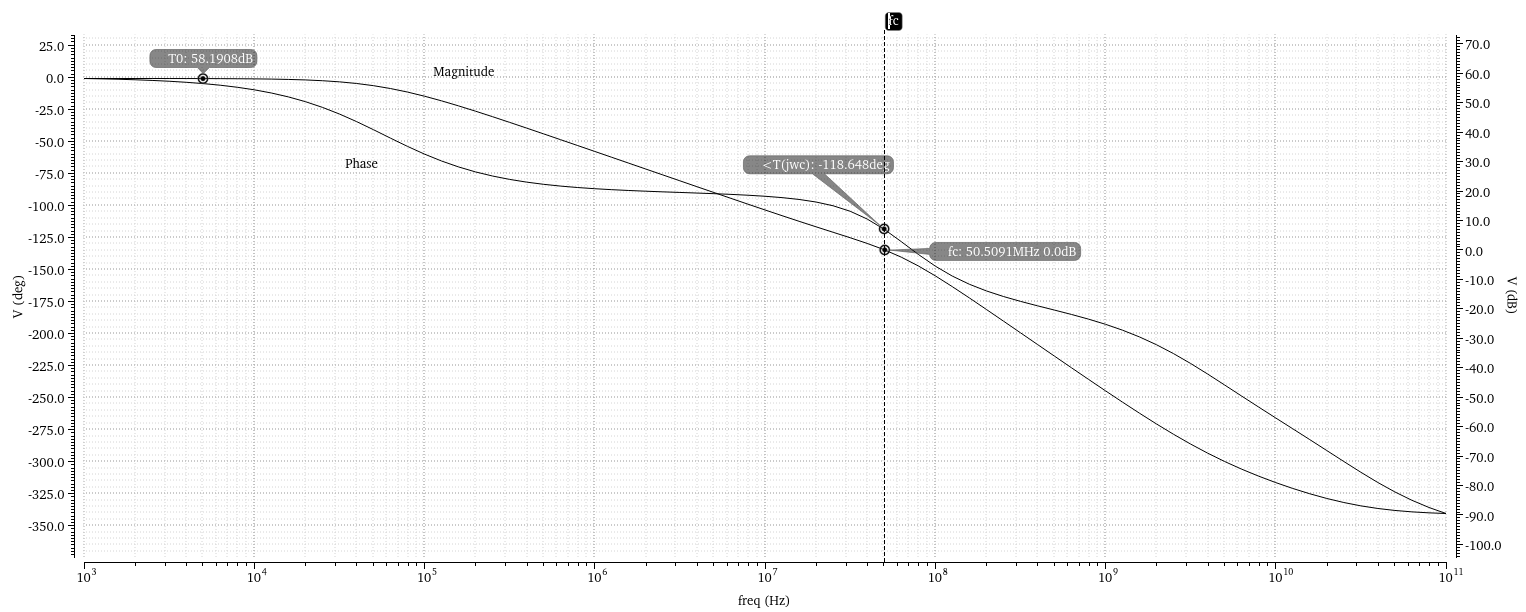
\includegraphics[width=0.85\textwidth]{immaginicorrettereport3/LOOPGAIN.png}
    \caption{Bode plot of the final loop transfer function.}
    \label{fig:loop_gain}
\end{figure}

The simulation yields $T_0=58.19\,\mathrm{dB}$, $f_c=50.51\,\mathrm{MHz}$, and $\angle T(j\omega_c)=-118.65^\circ$. The phase margin is thus calculated as:
\[
PM=180^\circ+\angle T(j\omega_c) = 180^\circ-118.65^\circ \simeq 61.35^\circ
\]
which satisfies the design specification ($60^\circ \leq PM \leq 70^\circ$).

Fig.~\ref{fig:loop_transient} shows the open-loop differential return signal $V_T(F_2)-V_T(F_1)$. The signal settles around $353\,\mathrm{mV}$, consistent with the low-frequency loop gain after the capacitive feedback network. Since the loop is opened for testbench analysis, this transient does not reflect the closed-loop settling behavior.

\begin{figure}[H]
    \centering
    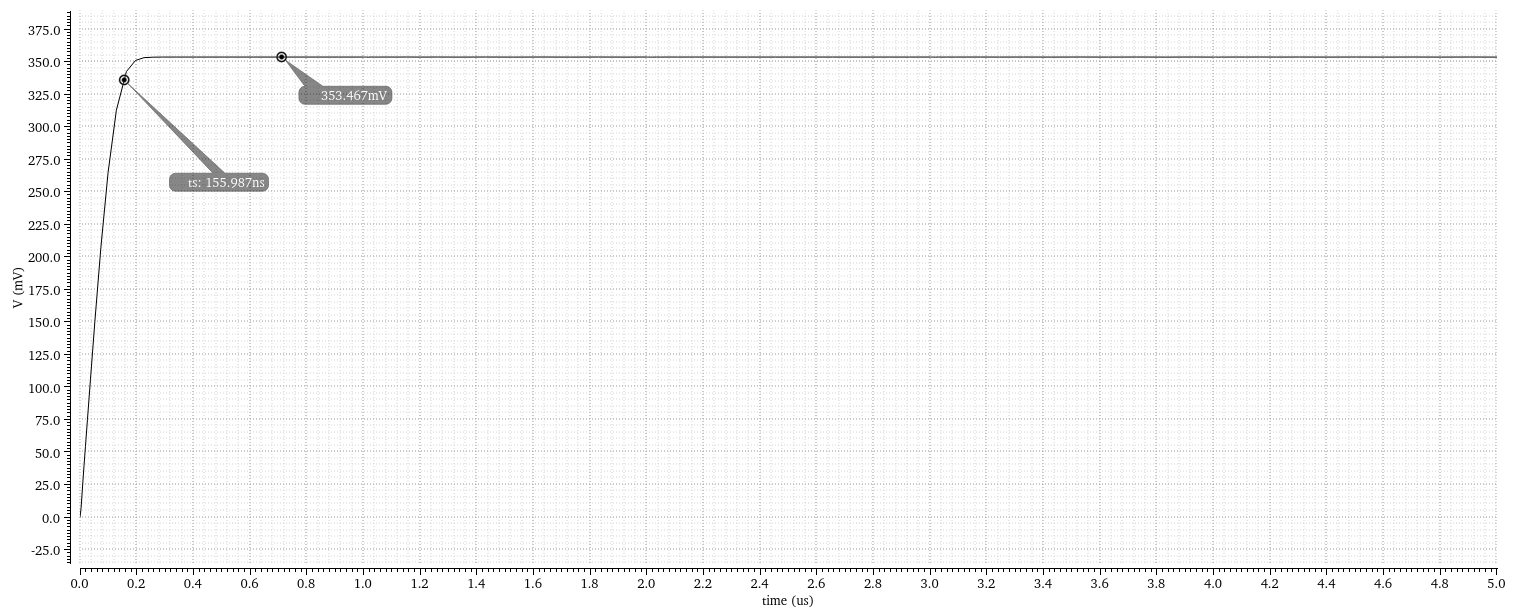
\includegraphics[width=0.85\textwidth]{immaginicorrettereport3/LOOP_DIFFERENTIAL_TRANSIENT.png}
    \caption{Transient response of the loop transfer function.}
    \label{fig:loop_transient}
\end{figure}

\subsection{Closed-Loop Feedback Amplifier Analysis}

The closed-loop differential transfer function of the capacitive feedback amplifier is plotted in Fig.~\ref{fig:closed_loop_bode}.

\begin{figure}[H]
    \centering
    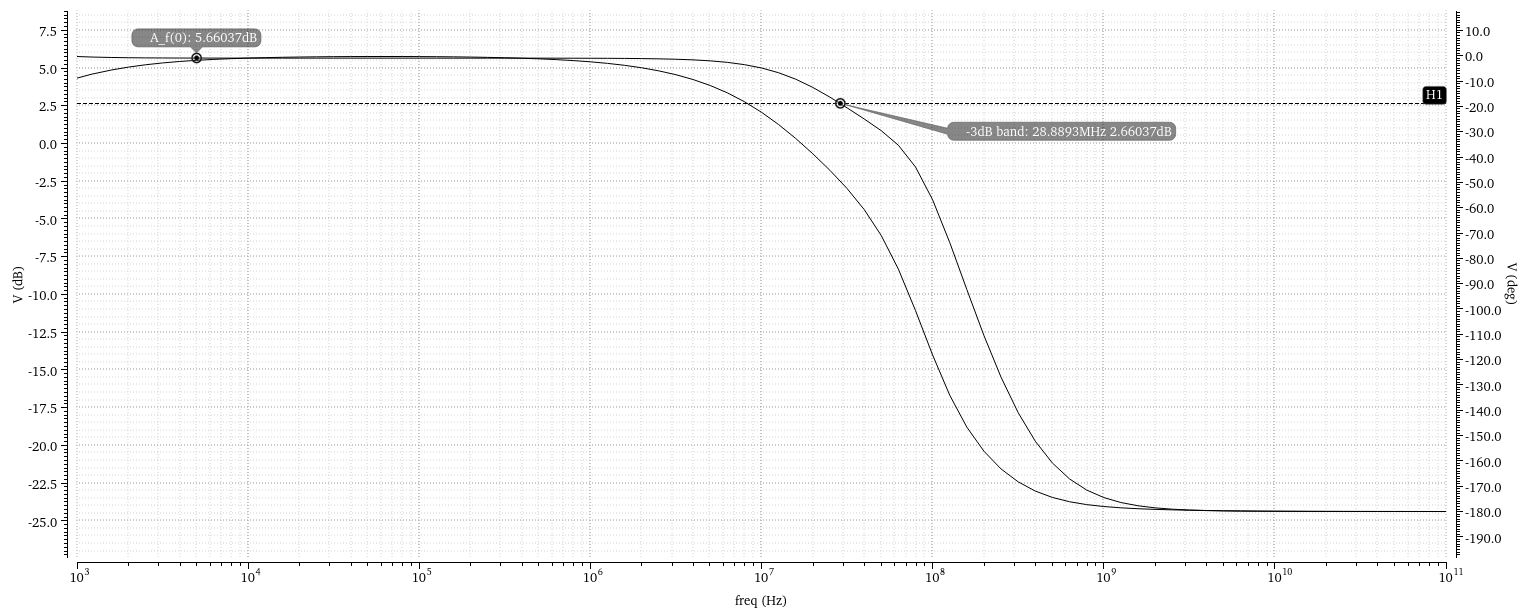
\includegraphics[width=0.85\textwidth]{immaginicorrettereport3/close_loop_differential.png}
    \caption{Bode plot of the closed-loop differential transfer function.}
    \label{fig:closed_loop_bode}
\end{figure}

The simulated low-frequency closed-loop gain is $A_{CL,0}=5.66\,\mathrm{dB}=1.92$. Compared to the ideal value set by the capacitive ratio ($A_{CL,ideal}=\frac{C_s}{C_f}=2$), the resulting static error is:
\[
\varepsilon_s= \left| \frac{A_{CL,ideal}-A_{CL,0}}{A_{CL,ideal}} \right| = \left| \frac{2-1.92}{2} \right| \simeq 4.1\%
\]
The measured $-3\,\mathrm{dB}$ bandwidth is $f_{-3\mathrm{dB}}\simeq28.89\,\mathrm{MHz}$.

\subsection{Closed-Loop Step Response and Dynamic Error}

\begin{figure}[H]
    \centering
    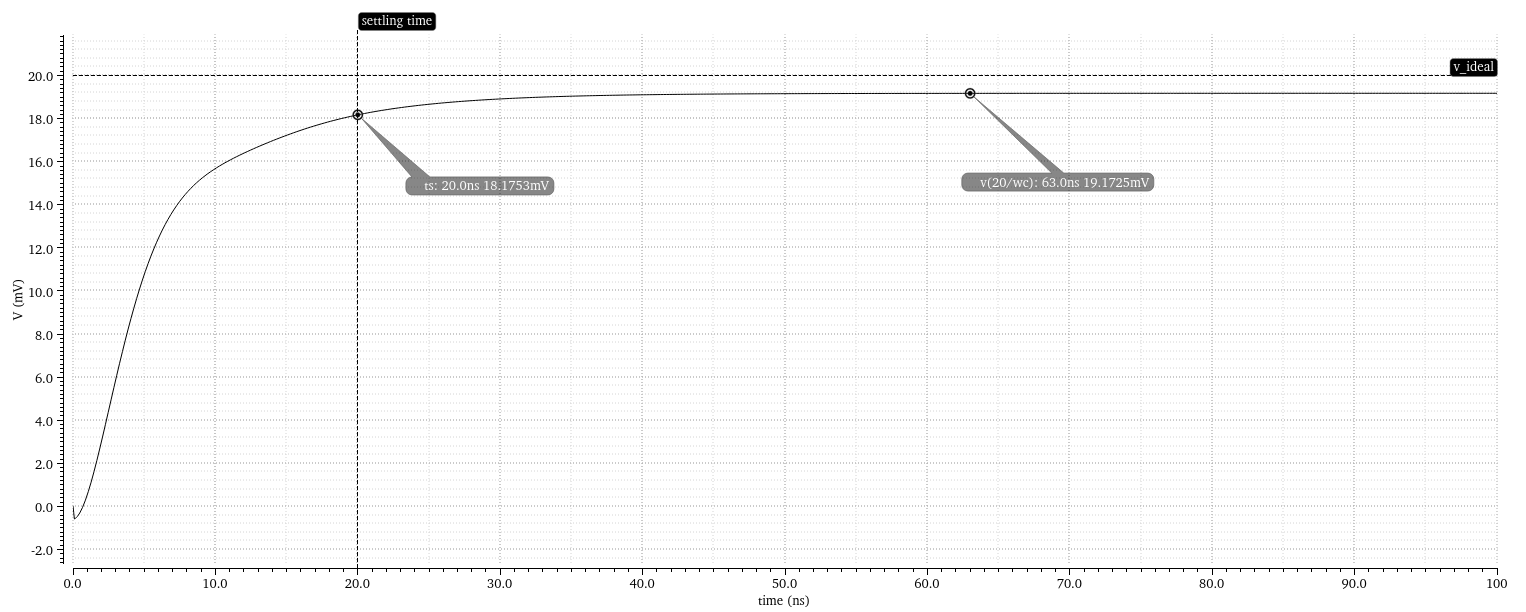
\includegraphics[width=0.85\textwidth]{immaginicorrettereport3/final_transient_response.png}
    \caption{Closed-loop differential step response of the final feedback amplifier.}
    \label{fig:closed_loop_transient}
\end{figure}

Fig.~\ref{fig:closed_loop_transient} shows the closed-loop step response to a $10\,\mathrm{mV}$ differential input step, where $V_{out,ideal}=20\,\mathrm{mV}$. The simulation reports $V_{out}(20\,\mathrm{ns})=18.175\,\mathrm{mV}$ and a settled value $V_{out}(\infty)\simeq19.173\,\mathrm{mV}$, yielding a dynamic error at $t_s=20\,\mathrm{ns}$ of:
\[
\varepsilon_d= \left| \frac{V_{out}(\infty)-V_{out}(20\,\mathrm{ns})}{V_{out}(\infty)} \right| = \frac{19.173-18.175}{19.173} \simeq 5.2\%
\]
This discrepancy arises because the theoretical first-order approximation $\varepsilon_d(t)\simeq e^{-\omega_c t}$ assumes a single dominant pole. In this OTA implementation, the second pole is close enough to the crossover frequency to introduce non-dominant exponential modes, slowing down the settling behavior and increasing the simulated dynamic error.



\subsection{Offset Voltage Estimation}

The OTA input-referred offset voltage was estimated via a 100-sample mismatch-only Monte Carlo simulation using the testbench shown in Fig.~\ref{fig:offset_tb}.

\begin{figure}[H]
    \centering
    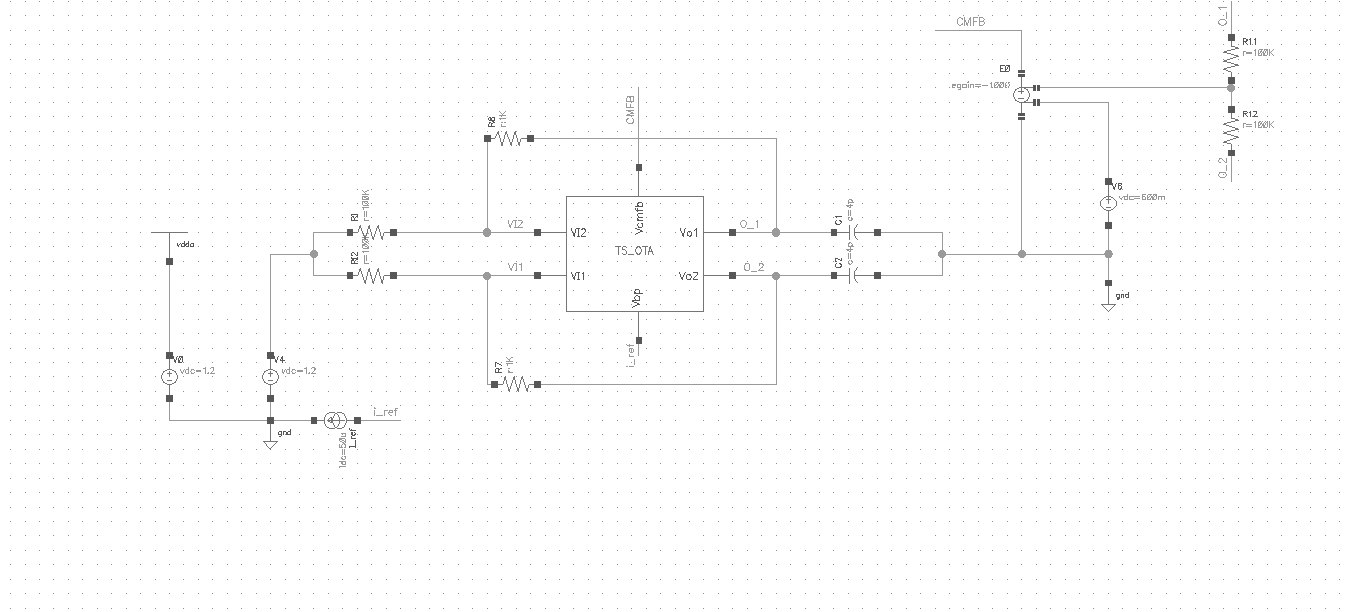
\includegraphics[width=0.85\textwidth]{immaginicorrettereport3/CORRECTMONTECARLO.png}
    \caption{Testbench employed for the Monte Carlo estimation of the input-referred offset voltage.}
    \label{fig:offset_tb}
\end{figure}

The resistive feedback network forces the OTA to operate close to equilibrium, while the high-gain loop minimizes the differential input voltage. Under the condition $\beta A_{dd0}\gg1$, the residual differential input voltage approximates the input-referred offset voltage:
\[
V_{ID}=V_{i2}-V_{i1}\approx V_{OS}
\]

The statistical distribution of the extracted differential input voltage is plotted in Fig.~\ref{fig:montecarlo_offset}.

\begin{figure}[H]
    \centering
    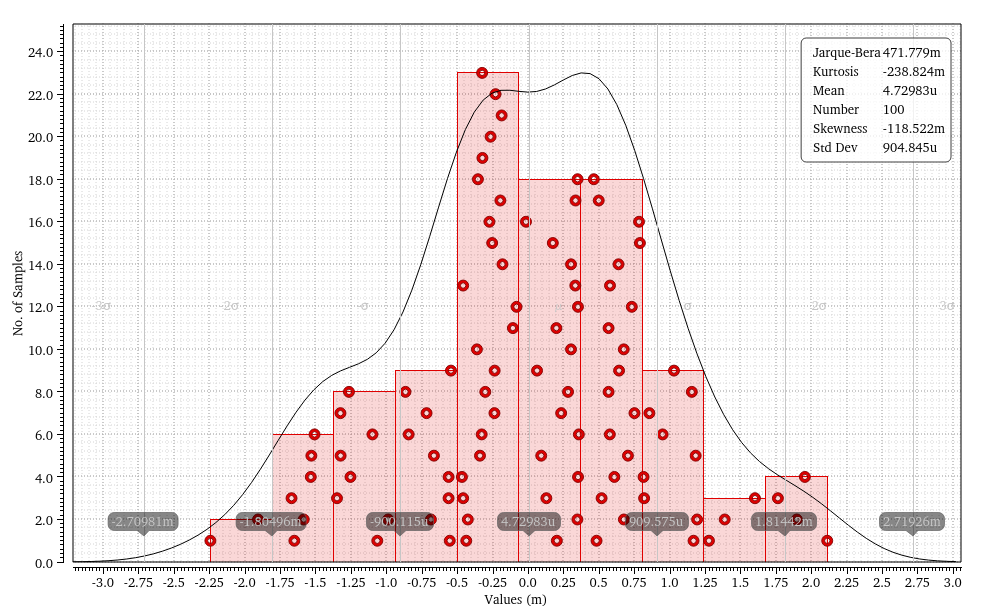
\includegraphics[width=0.85\textwidth]{immaginicorrettereport3/CORRECTMONTECARLONE.png}
    \caption{Monte Carlo distribution of the estimated input-referred offset voltage.}
    \label{fig:montecarlo_offset}
\end{figure}

The simulation yields a standard deviation of $\sigma(V_{ID})\simeq904.8\,\mu\mathrm{V}$. Therefore, the estimated input-referred offset voltage is:
\[
\boxed{V_{OS}\simeq0.905\,\mathrm{mV}}
\]
This complies with the design specification ($V_{OS}\leq2\,\mathrm{mV}$).
\section{Discussion of Unmet Specifications}

The final two-stage OTA design successfully optimized the trade-offs between speed, stability, and power consumption, satisfying the main specifications. The procedure was systematically developed from first-order analytical models, translating the static error target into a minimum loop gain ($\varepsilon_0\simeq\frac{1}{1+T_0}$) and the dynamic settling-time target into a minimum crossover frequency via the theoretical relation:
\[
\varepsilon_d(t_s)\simeq e^{-\omega_c t_s}
\]
This expression assumes an ideal first-order system where a single dominant pole governs the entire dynamics up to the crossover frequency.

The resulting system is not a simple single-pole network; consequently, the simulated closed-loop $-3\,\mathrm{dB}$ bandwidth ($f_{-3\mathrm{dB}}\simeq28.89\,\mathrm{MHz}$) deviated from the crossover frequency ($f_c\simeq50.51\,\mathrm{MHz}$). This non-ideality limited the settling behavior, causing the static error to settle at $4.1\%$ and the dynamic error at $5.2\%$, missing the highly conservative target of $0.2\%$. Pure first-order settling would ideally require a phase margin close to $90^\circ$ to completely suppress any non-dominant exponential mode. 


Moreover, the laboratory guidelines originally specified a required phase margin between $60^\circ$ and $70^\circ$. This initially motivated a compensation network targeting approximately $61.35^\circ$, yielding a moderately underdamped but fast transient response. After subsequent clarifications—obtained when the design and simulations were already completed—it was understood that the original specification contained an error and the intended requirement was a phase margin greater than $70^\circ$. This final interpretation is highly consistent with the theoretical framework of this report: a larger phase margin pushes the second pole higher, bringing the loop response closer to the dominant-pole behavior required by the first-order error equations.
\chapter{LAB Session 04 -- Low Voltage Band-Gap Voltage Reference}

\section{Preliminary Design of the LV-BGR}

\subsection{LV-BGR Schematic}

\begin{figure}[H]
    \centering
    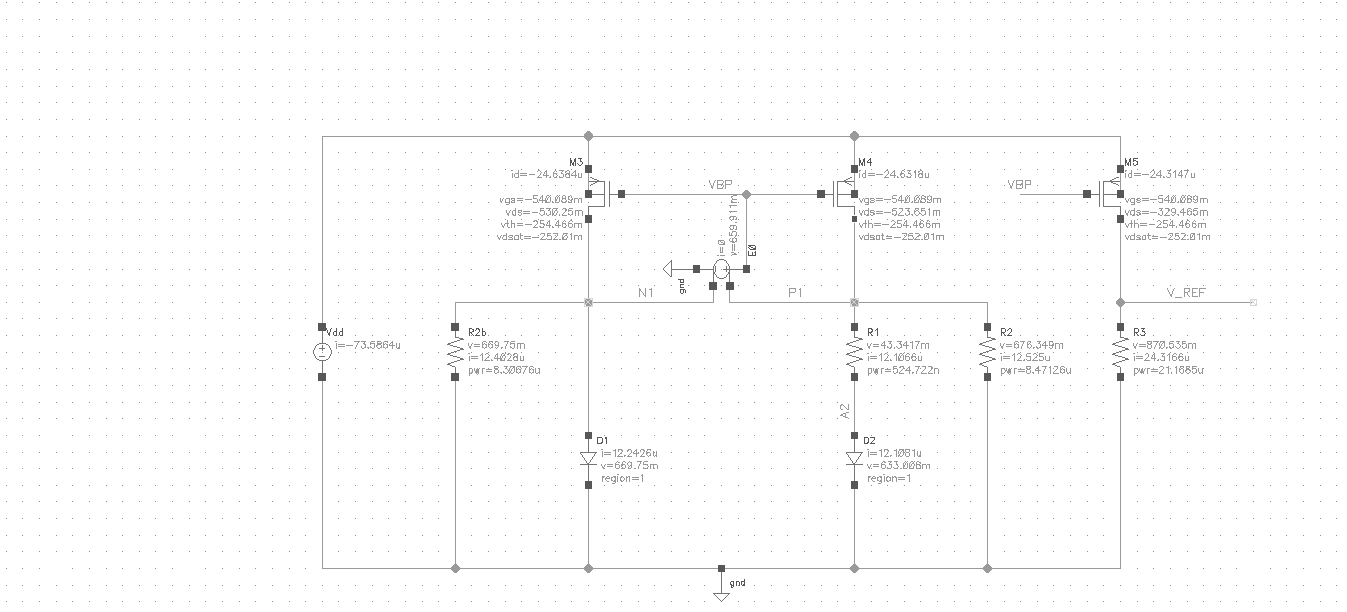
\includegraphics[width=\linewidth]{chapters/lab04/Schematic_LV_BGR.png}
    \caption{Schematic of the implemented LV-BGR.}
    \label{fig:lv_bgr_schematic}
\end{figure}

\subsection{Initial Sizing}

The preliminary design was obtained by imposing $I_1=10\,\mu\mathrm{A}$ and $N=\frac{A_{D2}}{A_{D1}}=4$. Since the OTA equalizes the two upper node voltages, the voltage across $R_1$ is $V_{R1}=V_{D1}-V_{D2}=U_T\ln(N)$, yielding $R_1=\frac{U_T\ln(N)}{I_1}\approx3.58\,\mathrm{k}\Omega$. Using the diode equation, the forward voltage of $D_1$ is estimated as $V_{D1}\approx0.665\,\mathrm{V}$.

The resistor $R_2$ controls the PTAT compensation term. Imposing $\frac{\partial V_{REF}}{\partial T}\approx0$ gives $R_2 = R_1 \frac{\ln(I_{S0}/I_1)}{\ln(N)} \approx54\,\mathrm{k}\Omega$. Finally, $R_3$ scales the output voltage to $V_{REF}=0.8\,\mathrm{V}$, requiring $R_3\approx35.8\,\mathrm{k}\Omega$. All resistors were implemented with a temperature coefficient of $TC_R=-5\cdot10^{-4}\,\mathrm{K}^{-1}$.

\subsection{PMOS Current Mirror Sizing}

The PMOS devices $M_3$, $M_4$, and $M_5$ form the bias current mirror. To reduce channel-length modulation, all transistors were initialized with $L=1.2\,\mu\mathrm{m}$. 

The mirror current is approximately $I_D=I_1+I_2$, where $I_2=\frac{V_{D1}}{R_2}\approx12.3\,\mu\mathrm{A}$, yielding $I_D\approx22.3\,\mu\mathrm{A}$. Assuming $|V_{OV}|=0.25\,\mathrm{V}$ for all transistors, the PMOS widths are estimated from the saturation current equation:
\[
W=\frac{2LI_D}{k_pV_{OV}^2}\approx8.6\,\mu\mathrm{m}
\]

\begin{table}[H]
\centering
\begin{tabular}{|c|c|c|c|}
\hline
\textbf{Component} & \textbf{R [k$\Omega$]} & \textbf{L [$\mu$m]} & \textbf{W [$\mu$m]} \\
\hline
M3 & -- & 1.2 & 8.6 \\
M4 & -- & 1.2 & 8.6 \\
M5 & -- & 1.2 & 8.6 \\
R1 & 3.58 & -- & -- \\
R2 & 54 & -- & -- \\
R3 & 35.8 & -- & -- \\
\hline
\end{tabular}
\caption{Initial sizing parameters of the LV-BGR.}
\label{tab:lvbgr_initial_sizing}
\end{table}

\subsection{PTAT and CTAT Characterization}

All the following temperature coefficients were evaluated locally around $27^\circ\mathrm{C}$, using close markers, since some curves are not perfectly linear. A DC temperature sweep from $-40^\circ\mathrm{C}$ to $85^\circ\mathrm{C}$ was performed to verify the CTAT and PTAT quantities.

\begin{figure}[H]
    \centering
    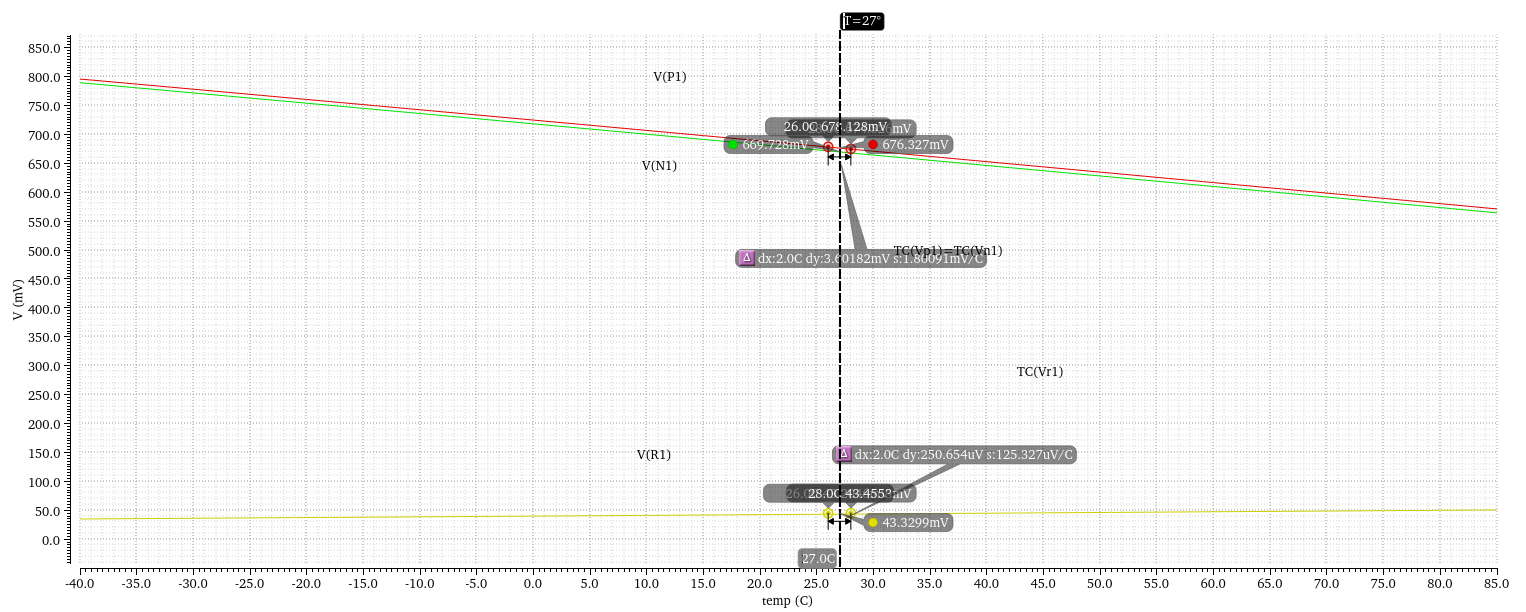
\includegraphics[width=\linewidth]{chapters/lab04/plot1.png}
    \caption{CTAT node voltages and PTAT voltage across $R_1$.}
    \label{fig:plot1}
\end{figure}

The diode voltages $V_{N1}$ and $V_{P1}$ show the expected CTAT behavior:
\[
\frac{dV_D}{dT}\approx -1.80\,\mathrm{mV/^\circ C}.
\]
The voltage across $R_1$, $V_{PTAT}=V(P1)-V(A2)$, increases with temperature, confirming the PTAT generation:
\[
\frac{dV_{PTAT}}{dT}\approx 125\,\mu\mathrm{V/^\circ C}.
\]

\subsection{Current Characterization}

\begin{figure}[H]
    \centering
    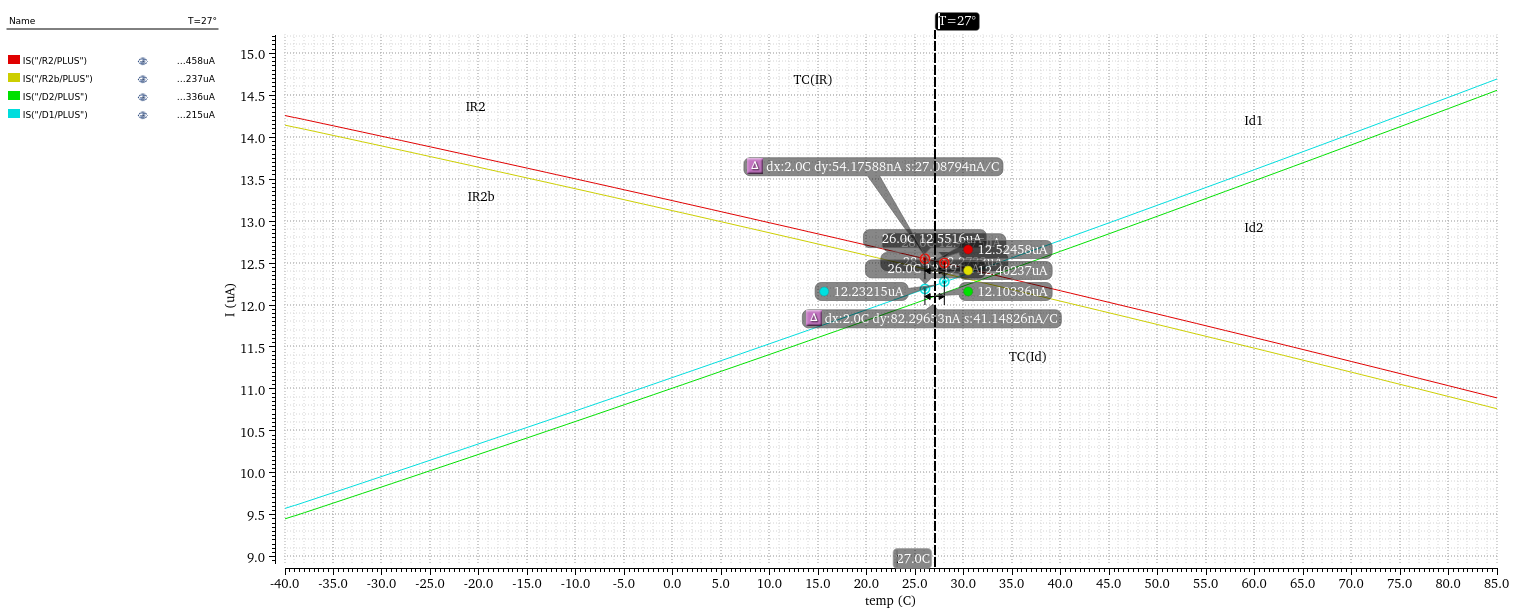
\includegraphics[width=\linewidth]{chapters/lab04/plot2.png}
    \caption{Internal branch currents versus temperature.}
    \label{fig:plot2}
\end{figure}

The diode currents $I_{D1}$ and $I_{D2}$ are almost equal, confirming the correct operation of the OTA feedback loop and of the PMOS current mirror. Around room temperature, the extracted slopes are approximately:
\[
\frac{dI_D}{dT}\approx 41\,\mathrm{nA/^\circ C},
\qquad
\frac{dI_{R2}}{dT}\approx 27\,\mathrm{nA/^\circ C}.
\]
However, the simulated diode current is still larger than the target value $I_1=10\,\mu\mathrm{A}$, therefore $R_1$ must be tuned.

\subsection{Initial Reference Voltage Characterization}

\begin{figure}[H]
    \centering
    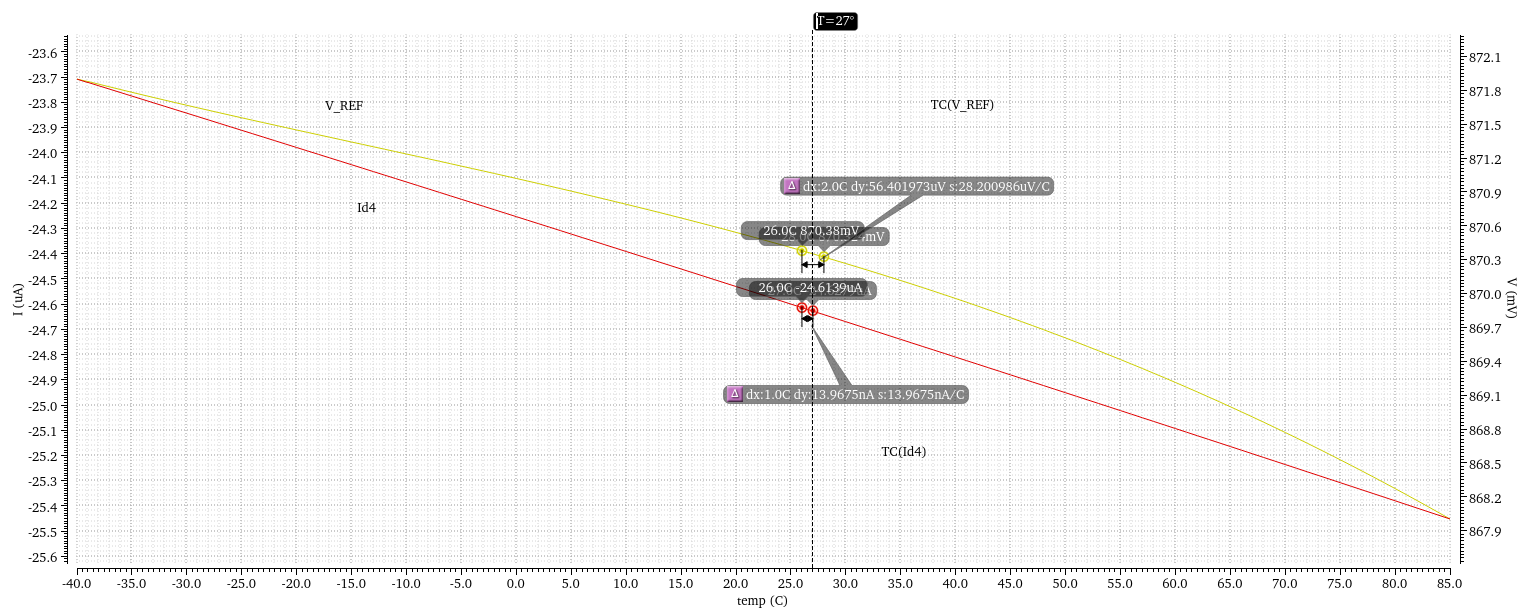
\includegraphics[width=\linewidth]{chapters/lab04/plot3.png}
    \caption{Initial $V_{REF}$ and $I_{D4}$ versus temperature.}
    \label{fig:plot3}
\end{figure}

The preliminary design generates a reference voltage close to the desired range, but still affected by a residual temperature dependence. Around $27^\circ\mathrm{C}$:
\[
V_{REF}\approx 870.4\,\mathrm{mV},
\]
\[
\frac{dV_{REF}}{dT}\approx 28.2\,\mu\mathrm{V/^\circ C},
\qquad
TC_{VREF}\approx 32\,\mathrm{ppm/^\circ C}.
\]
The PMOS mirror current shows a local slope of about:
\[
\frac{dI_{D4}}{dT}\approx 14\,\mathrm{nA/^\circ C}.
\]

\paragraph{Assessment of the Preliminary Design}
The preliminary design already exhibits the expected CTAT and PTAT behaviors. At room temperature, the simulated branch current is $I_{D1}=12.31\,\mu\mathrm{A}$, compared to the target value of $10\,\mu\mathrm{A}$, while the reference voltage is $V_{REF}=870.4\,\mathrm{mV}$ instead of the specified $800\,\mathrm{mV}$. Moreover, the extracted temperature coefficient is $TC_{VREF}\approx32\,\mathrm{ppm/^\circ C}$, which is significantly larger than the target specification. These deviations are mainly due to the approximations adopted in the hand calculations and to device non-idealities included in the simulation models. Therefore, a tuning procedure is required to meet the design specifications.


\section{Resistors Tuning}

The resistor values were then tuned sequentially. $R_1$ sets the PTAT current, $R_2$ controls the PTAT/CTAT compensation, and $R_3$ sets the final absolute value of $V_{REF}$.

\subsection{Tuning of $R_1$}

The theoretical value $R_1=3.58\,\mathrm{k}\Omega$ produced $I_{D1}=12.31\,\mu\mathrm{A}$, larger than the target current $I_1=10\,\mu\mathrm{A}$. Since the branch current is approximately inversely proportional to $R_1$, the resistor was increased to:
\[
\boxed{R_1=4.346\,\mathrm{k}\Omega}
\]
obtaining $I_{D1}=10.0018\,\mu\mathrm{A}$.

\begin{figure}[H]
    \centering
    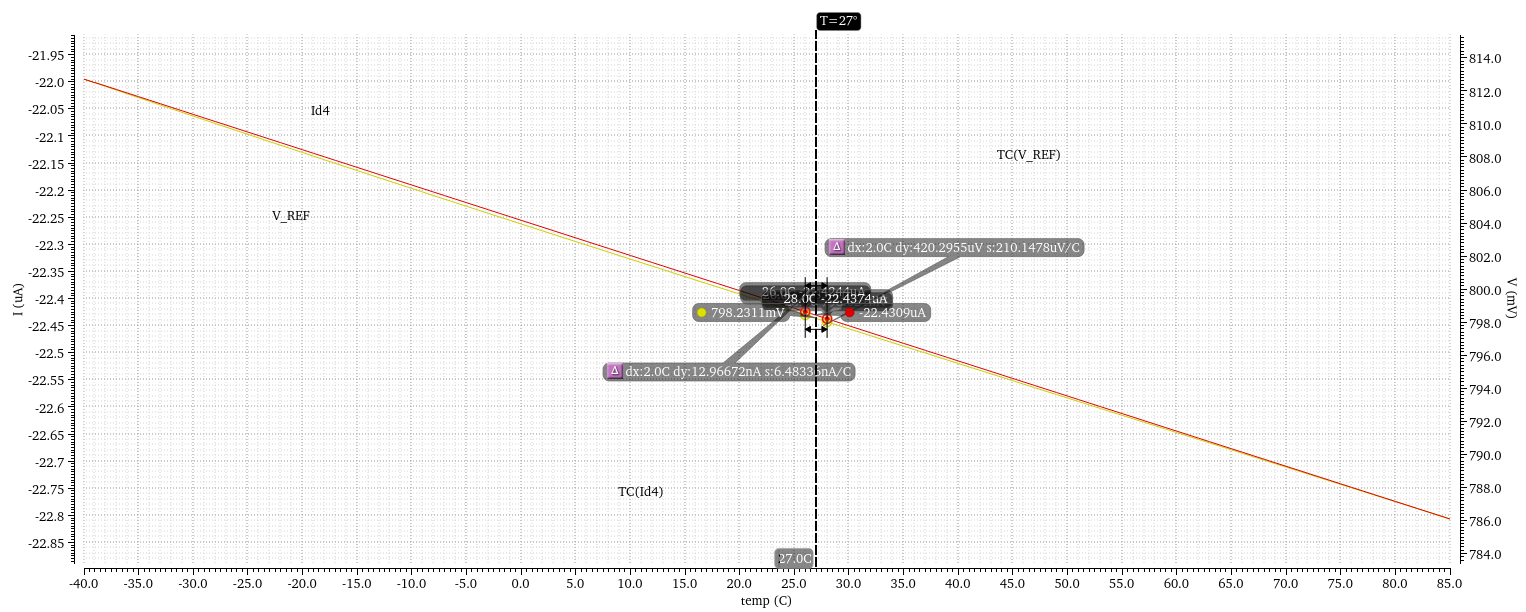
\includegraphics[width=\linewidth]{chapters/lab04/tuning1.png}
    \caption{$V_{REF}$ and $I_{D4}$ after tuning $R_1$.}
    \label{fig:tuning1}
\end{figure}

After this step, $V_{REF}$ still shows a significant temperature slope:
\[
\frac{dV_{REF}}{dT}\approx 210\,\mu\mathrm{V/^\circ C}.
\]
This indicates that the PTAT/CTAT compensation must be adjusted through $R_2$.

\subsection{Tuning of $R_2$}

The resistor $R_2$ controls the weight of the PTAT term added to the CTAT diode voltage:
\[
V_{REF}\propto V_{D1}+\frac{R_2}{R_1}U_T\ln(N).
\]
Therefore, increasing $R_2$ increases the PTAT contribution. A parametric sweep was performed on both matched resistors $R_2=R_{2b}$. First, a coarse sweep was performed:
\[
54\,\mathrm{k}\Omega \leq R_2 \leq 70\,\mathrm{k}\Omega,
\qquad
\Delta R_2=1\,\mathrm{k}\Omega.
\]

\begin{figure}[H]
    \centering
    \includegraphics[width=\linewidth]{chapters/lab04/tuning2a.png}
    \caption{Coarse parametric sweep of $R_2$.}
    \label{fig:tuning2a}
\end{figure}

The minimum local slope was found around $R_2=66\,\mathrm{k}\Omega$. A refined sweep was then performed around this region:
\[
64\,\mathrm{k}\Omega \leq R_2 \leq 70\,\mathrm{k}\Omega,
\qquad
\Delta R_2=0.2\,\mathrm{k}\Omega.
\]

\begin{figure}[H]
    \centering
    \includegraphics[width=\linewidth]{chapters/lab04/tuning2b.png}
    \caption{Refined parametric sweep of $R_2$.}
    \label{fig:tuning2b}
\end{figure}

The selected value is:
\[
\boxed{R_2=R_{2b}=66\,\mathrm{k}\Omega}.
\]

\begin{figure}[H]
    \centering
    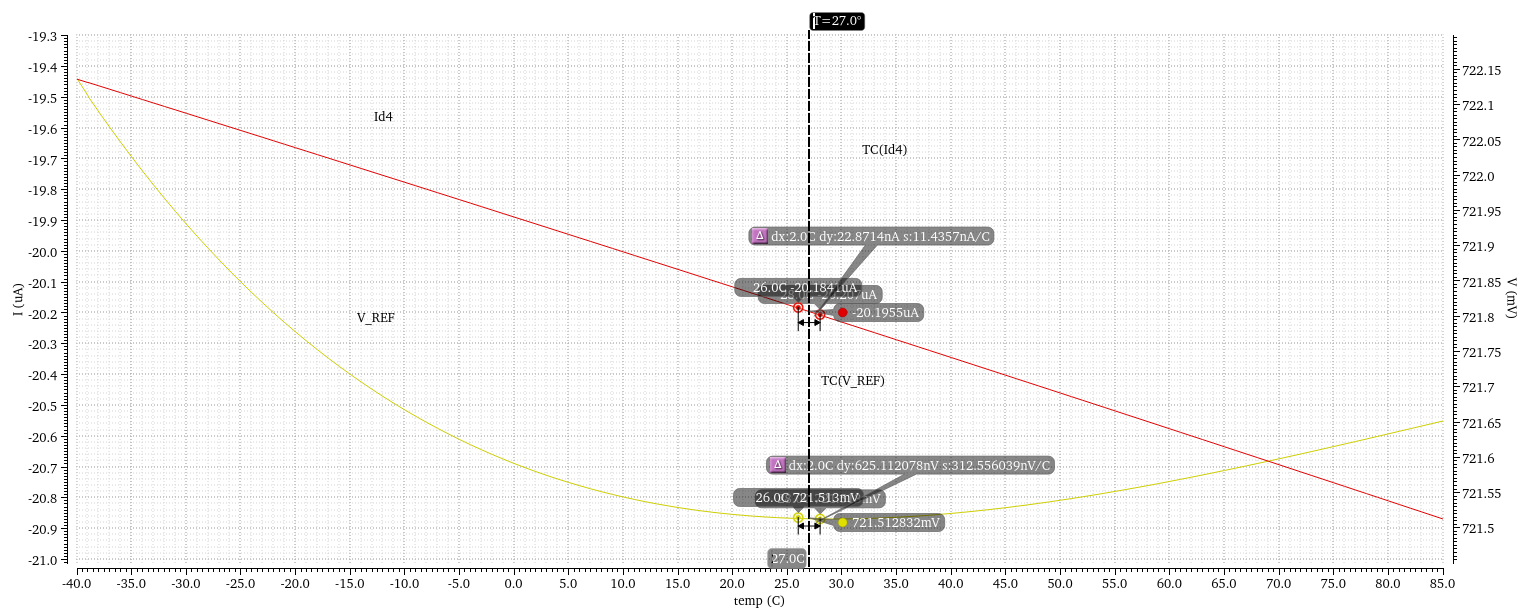
\includegraphics[width=\linewidth]{chapters/lab04/tuning2c.png}
    \caption{$V_{REF}$ and $I_{D4}$ after tuning $R_2$.}
    \label{fig:tuning2c}
\end{figure}

With this value, the local temperature coefficient of $V_{REF}$ is strongly reduced:
\[
\frac{dV_{REF}}{dT}\approx 0.31\,\mu\mathrm{V/^\circ C}.
\]
The resulting $V_{REF}(T)$ characteristic is not perfectly linear and exhibits a slight second-order curvature. This behavior is mainly due to second-order effects neglected in the hand calculations, especially the temperature dependence of model parameters such as $I_{S0}$. Nevertheless, the tuning of $R_2$ allows the operating point around room temperature to lie close to the minimum of the parabola, where the local temperature coefficient is minimized.

\subsection{Tuning of $R_3$}

After the compensation was optimized through $R_2$, $R_3$ was tuned to set the absolute value of the reference voltage. Since $V_{REF}\approx \frac{R_3}{R_2}V_{G0}$, $R_3$ directly scales the output reference. A parametric sweep was performed around the expected value:
\[
39.7\,\mathrm{k}\Omega \leq R_3 \leq 40.0\,\mathrm{k}\Omega.
\]

\begin{figure}[H]
    \centering
    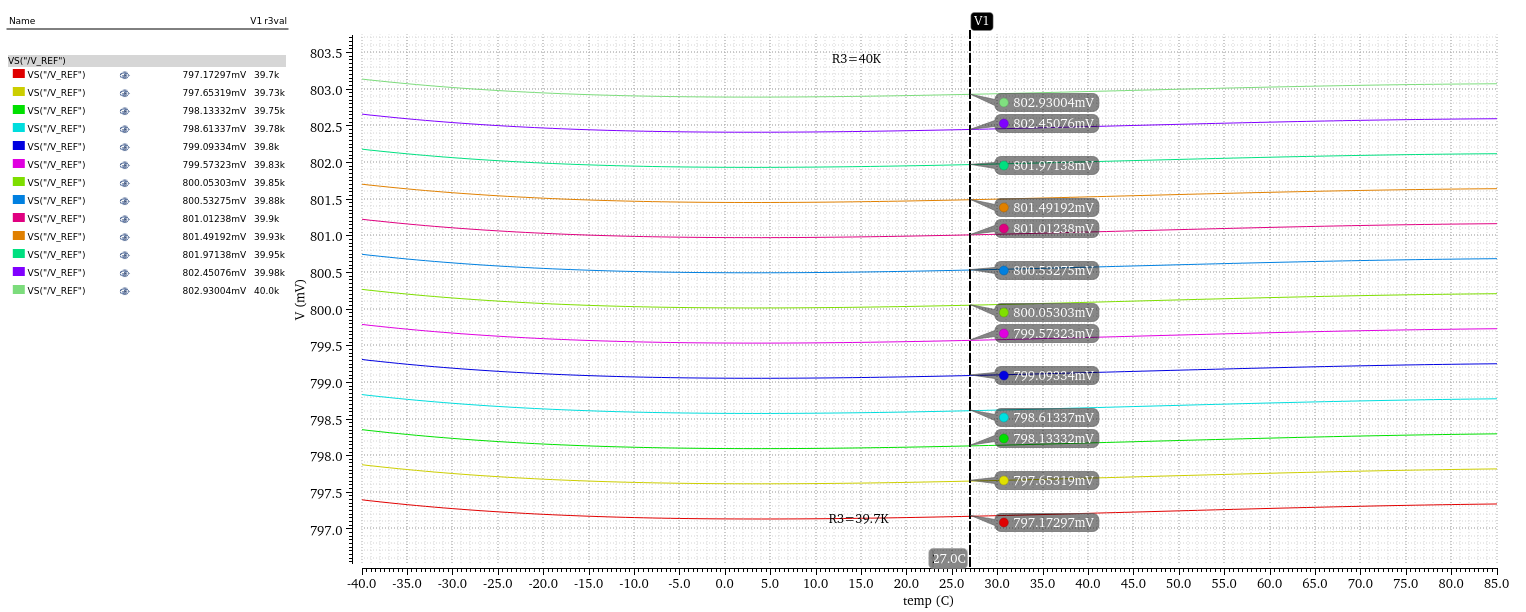
\includegraphics[width=\linewidth]{chapters/lab04/tuning3a.png}
    \caption{Parametric sweep of $R_3$ for setting $V_{REF}=0.8\,\mathrm{V}$.}
    \label{fig:tuning3a}
\end{figure}

The selected value is:
\[
\boxed{R_3=39.85\,\mathrm{k}\Omega}.
\]
The final temperature sweep is shown in Figure~\ref{fig:tuning3b}.

\begin{figure}[H]
    \centering
    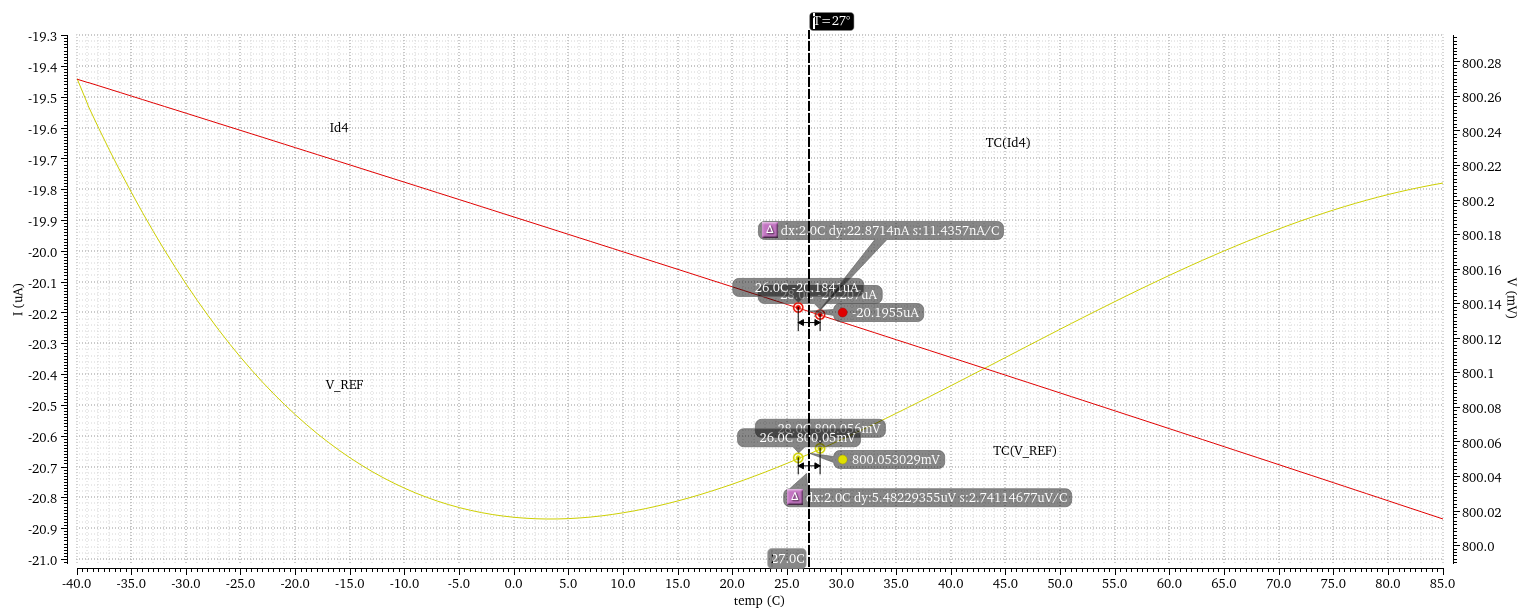
\includegraphics[width=\linewidth]{chapters/lab04/tuning3b.png}
    \caption{Final $V_{REF}$ and $I_{D4}$ after tuning $R_3$.}
    \label{fig:tuning3b}
\end{figure}

At room temperature:
\[
V_{REF}(27^\circ\mathrm{C})\approx800.05\,\mathrm{mV},
\qquad
\frac{dV_{REF}}{dT}\approx2.74\,\mu\mathrm{V/^\circ C},
\]
thus
\[
TC_{VREF} = \frac{1}{V_{REF}}\frac{dV_{REF}}{dT} \approx3.4\,\mathrm{ppm/^\circ C}.
\]
The $V_{REF}(T)$ characteristic exhibits a slight second-order curvature due to effects neglected in the hand calculations, mainly the temperature dependence of parameters such as $I_{S0}$. Nevertheless, the tuning keeps the room-temperature operating point on the flat part of the parabola, where the local temperature coefficient is small.

Since the local slope depends on where it is evaluated, the reference is also characterised over the whole temperature range with the box method:
\[
TC_{VREF}^{box} = \frac{V_{REF,max}-V_{REF,min}}{V_{REF}(27^\circ\mathrm{C})\,(T_{max}-T_{min})}
\approx \frac{800.27\,\mathrm{mV}-800.02\,\mathrm{mV}}{800.05\,\mathrm{mV}\cdot125^\circ\mathrm{C}}
\approx 2.5\,\mathrm{ppm/^\circ C},
\]
where $V_{REF,max}$ occurs at $-40^\circ\mathrm{C}$ and $V_{REF,min}$ at about $0^\circ\mathrm{C}$. Over the full $-40$ to $85^\circ\mathrm{C}$ range, the total variation is only about $0.25\,\mathrm{mV}$. The vertex of the parabola sits near $0^\circ\mathrm{C}$ rather than at the centre of the range ($22.5^\circ\mathrm{C}$). A slightly smaller $R_2$, which reduces the PTAT contribution, would move the vertex towards the centre and balance the two ends, lowering the box-method coefficient further.

Similarly,
\[
I_{D4}(27^\circ\mathrm{C})\approx20.20\,\mu\mathrm{A},
\qquad
\frac{dI_{D4}}{dT}\approx11.4\,\mathrm{nA/^\circ C}.
\]
Unlike $V_{REF}$, the internal branch currents are not directly optimized for temperature compensation. Therefore, a residual temperature dependence of $I_{D4}$ is expected after the tuning procedure.


\section{$V_{DD}$ Sensitivity}

Finally, the dependence of the reference voltage on the supply voltage was evaluated by performing a $V_{DD}$ sweep around its nominal value $1.2\,\mathrm{V}$. As required by the laboratory specifications, the supply voltage was varied within a $\pm10\%$ range:
\[
1.08\,\mathrm{V} \leq V_{DD} \leq 1.32\,\mathrm{V}.
\]

\begin{figure}[H]
    \centering
    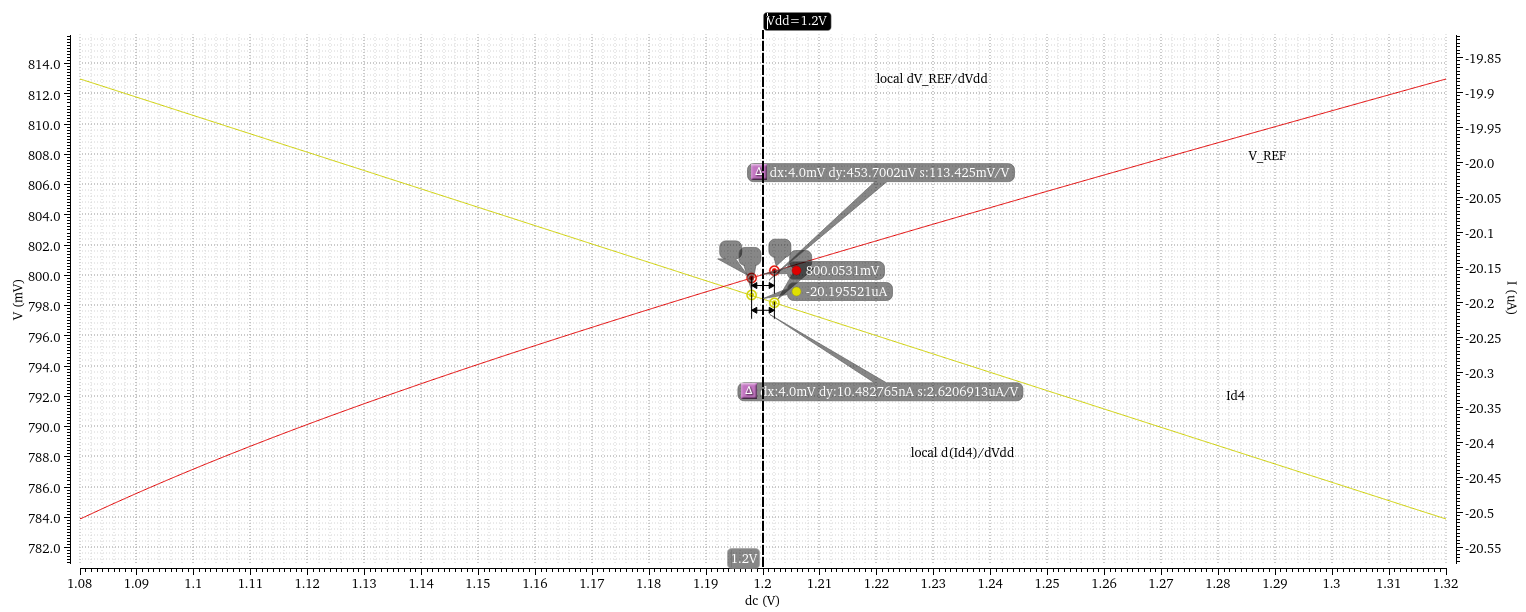
\includegraphics[width=\linewidth]{chapters/lab04/FINALFIG.png}
    \caption{$V_{REF}$ and $I_{D4}$ sensitivity to $V_{DD}$.}
    \label{fig:vdd_sensitivity}
\end{figure}

At $V_{DD}=1.2\,\mathrm{V}$, the reference voltage is approximately $V_{REF}\approx800.05\,\mathrm{mV}$. Using local markers around the nominal supply voltage, the sensitivity was estimated as:
\[
\frac{dV_{REF}}{dV_{DD}} \approx \frac{V_{REF}(1.202\,\mathrm{V})-V_{REF}(1.198\,\mathrm{V})}{4\,\mathrm{mV}} \approx113\,\mathrm{mV/V}.
\]

Similarly, the PMOS mirror current sensitivity is:
\[
\frac{dI_{D4}}{dV_{DD}} \approx \frac{I_{D4}(1.202\,\mathrm{V})-I_{D4}(1.198\,\mathrm{V})}{4\,\mathrm{mV}} \approx2.62\,\mu\mathrm{A}/\mathrm{V}.
\]
The final design therefore shows a good robustness against temperature variations, achieving a low local temperature coefficient around room temperature. On the other hand, the reference voltage is more sensitive to supply variations, as expected for a simple bandgap architecture without dedicated enhancement techniques.


\section{Final design verification}

The final design provides a reference voltage of $V_{REF}(27^\circ\mathrm{C})\approx800.05\,\mathrm{mV}$ with a local temperature coefficient of $TC_{VREF}\approx3.4\,\mathrm{ppm/^\circ C}$ at room temperature and a box-method coefficient of about $2.5\,\mathrm{ppm/^\circ C}$ over $-40$ to $85^\circ\mathrm{C}$ (total variation $\approx0.25\,\mathrm{mV}$). Although slightly higher than the target specification of $2\,\mathrm{ppm/^\circ C}$, this result confirms the effectiveness of the PTAT/CTAT compensation strategy and highlights the impact of second-order temperature effects neglected in the analytical derivation.

The dependence of the reference voltage on the supply voltage was also evaluated. Around the nominal supply voltage ($V_{DD}=1.2\,\mathrm{V}$), the measured sensitivity is:
\[
\frac{\mathrm{d}V_{REF}}{\mathrm{d}V_{DD}} \approx 113\,\mathrm{mV/V}
\]







\end{document}